\documentclass[a4paper, UKenglish, 11pt, twoside]{report}
\usepackage[utf8]{inputenc}
\usepackage[T1]{fontenc}
\usepackage{babel}
\usepackage[UKenglish]{uiomasterfp/uiomasterfp}

%Citation Packages
\usepackage{csquotes}
\usepackage[backend=bibtex]{biblatex}
\usepackage{silence}
\WarningFilter{biblatex}{File 'UKenglish-plain.lbx'}
\bibliography{../References/abbrev0.bib, ../References/crypto.bib, ../References/ref.bib}


\usepackage{float}
\usepackage{amsmath}
\usepackage{amsfonts}
\usepackage{amssymb}
\usepackage{chngcntr}
\counterwithout{equation}{chapter}
\usepackage[flushleft]{threeparttable}
\usepackage{tabularx}
\usepackage[hidelinks]{hyperref}
\usepackage{enumitem}
\usepackage{algorithm2e}
\usepackage{siunitx}
\usepackage{breqn}
\usepackage{tikz}
\usepackage{pgfplots}
\pgfplotsset{compat=1.18}
\usepackage{multirow}
\usepackage{caption}
\usepackage{listings}
\usepackage{etoolbox}
\usepackage{nameref}
\usepackage[capitalise, noabbrev]{cleveref}
\usepackage[justification=centering]{caption}
\usepackage{xurl}
\DeclareMathAlphabet{\mathpzc}{OT1}{pzc}{m}{it}
\usepackage[acronym,nonumberlist]{glossaries}
\makenoidxglossaries
\usepackage{bm}

\newcommand\Tstrut{\rule{0pt}{0.5ex}}
\newcommand\Bstrut{\rule[2ex]{0pt}{0pt}}

\newacronym{aes}{AES}{Advanced Encryption Standard}
\newacronym{ca}{CA}{Certificate Authority}
\newacronym{cpu}{CPU}{Central Processing Unit}
\newacronym{ctr}{CTR}{Counter}
\newacronym{ddh}{DDH}{Decisional Diffie-Hellman}
\newacronym{ecb}{ECB}{Electronic Code Book}
\newacronym{xor}{XOR}{Exclusive OR}
\newacronym{ifi}{IFI}{Department of Informatics}
\newacronym{ffi}{FFI}{Norwegian Defence Research Establishment}
\newacronym{cpds}{cPDS}{computational Private Database Search}
\newacronym{indcca}{IND-CCA}{Indistinguishable under Chosen Ciphertext Attack}
\newacronym{indcpa}{IND-CPA}{Indistinguishable under Chosen Plaintext Attack}
\newacronym{ip}{IP}{Internet Protocol}
\newacronym{lan}{LAN}{Local Area Network}
\newacronym{llm}{LLM}{Large Language Model}
\newacronym{mpc}{MPC}{(Secure) Multi-Party Computation}
\newacronym{oeis}{OEIS}{The On-line Encyclopedia of Integer Sequences}
\newacronym{oprf}{OPRF}{Oblivious Pseudorandom Function}
\newacronym{oram}{ORAM}{Oblivious Random Access Machine}
\newacronym{ot}{OT}{Oblivious Transfer}
\newacronym{uio}{UiO}{University of Oslo}
\newacronym{pdq}{PDQ}{Private Database Query}
\newacronym{pds}{PDS}{Private Database Search}
\newacronym{pir}{PIR}{Private Information Retrieval}
\newacronym{pnr}{PNR}{Passenger Name Record}
\newacronym{ppt}{PPT}{Probabilistic Polynomial-Time}
\newacronym{psi}{PSI}{Private Set Intersection}
\newacronym{ps}{PS}{Private Swap}
\newacronym{ram}{RAM}{Random Access Memory}
\newacronym{sbert}{SBERT}{Sentence-BERT}
\newacronym{shake}{SHAKE}{Secure Hash Algorithm and KECCAK}
\newacronym{she}{SHE}{Somewhat Homomorphic Encryption}
\newacronym{spir}{SPIR}{Symmetric Private Information Retrieval}
\newacronym{tls}{TLS}{Transport Layer Security}
\newacronym{wlan}{WLAN}{Wireless Local Area Network}

\newglossaryentry{a}
{
    name={$ A $},
    description={Auxiliary information about the database, $ A \in {\lbrace 0, 1 \rbrace}^\rho $}
}
\newglossaryentry{aa}
{
    name={$ A' $},
    description={The encoded auxiliary information $ A $}
}
\newglossaryentry{aaa}
{
    name={$ \mathcal{A} $},
    description={A probabilistic polynomial-time algorithm used to denote an adversary},
    sort=A
}
\newglossaryentry{aaaa}
{
    name={$ \alpha $},
    description={Additional time spent on landing and take-off when flying between two airports}
}
\newglossaryentry{b}
{
    name={$ b $},
    description={A single bit, 0 or 1}
}
\newglossaryentry{bb}
{
    name={$ b' $},
    description={The adversary's prediction bit, 0 or 1}
}
\newglossaryentry{bbb}
{
    name={$ \beta $},
    description={The block size}
}
\newglossaryentry{c}
{
    name={$ C_i / C_j $},
    description={A ciphertext}
}
\newglossaryentry{cc}
{
    name={$ C'_i / C'_j $},
    description={A masked ciphertext}
}
\newglossaryentry{ccc}
{
    name={$ \mathcal{C} $},
    description={A circuit description of a function},
    sort=C
}
\newglossaryentry{cccc}
{
    name={$ c_i / c_j $},
    description={A counter}
}
\newglossaryentry{ccccc}
{
    name={$ \chi $},
    description={The length of the search query $ q $. $ \chi \in \mathbb{Z}^+ $}
}
\newglossaryentry{d}
{
    name={$ D $},
    description={The database}
}
\newglossaryentry{dd}
{
    name={$ D' $},
    description={The encoded database}
}
\newglossaryentry{ddd}
{
    name={$ d_i $},
    description={A dummy record}
}
\newglossaryentry{dddd}
{
    name={$ \delta $},
    description={Distance between two vectors}
}
\newglossaryentry{e}
{
    name={$ E $},
    description={An encryption scheme}
}
\newglossaryentry{ee}
{
    name={$ \mathcal{E} \left( \lambda \right) $},
    description={A negligible function $ \mathcal{E}: \mathbb{N} \mapsto \mathbb{R}^+ $ that takes the security parameter $ \lambda $},
    sort=E
}
\newglossaryentry{eee}
{
    name={$ e_i / e_{i,j} $},
    description={An encryption encryption key}
}
\newglossaryentry{eeee}
{
    name={$ \eta $},
    description={The set of dummy record indices}
}
\newglossaryentry{f}
{
    name={$ F $},
    description={The retrieved records, $ F \subset D $}
}
\newglossaryentry{ff}
{
    name={$ F' $},
    description={The retrieved encrypted records}
}
\newglossaryentry{g}
{
    name={$ \mathcal{G} $},
    description={A garbled circuit},
    sort=g
}
\newglossaryentry{gg}
{
    name={$ \Gamma $},
    description={A large language model that outputs vector embeddings}
}
\newglossaryentry{ggg}
{
    name={$ \gamma_i $},
    description={A vector embedding produce with $ \Gamma $}
}
\newglossaryentry{h}
{
    name={$ H $},
    description={A history of responses}
}
\newglossaryentry{i}
{
    name={$ I / I_i / I_j $},
    description={A set of indices, $ I \in {\lbrace 1, 2, ... , n \rbrace}^\nu $}
}
\newglossaryentry{ii}
{
    name={$ I' / I'_i / I'_j $},
    description={A set of encoded indices, $ I' \in {\lbrace 1, 2, ... , n \rbrace}^\sigma $}
}
\newglossaryentry{iii}
{
    name={$ i $},
    description={An index or iteration, $ i \in {\lbrace 1, 2, ... , n \rbrace} $}
}
\newglossaryentry{iiii}
{
    name={$ i' $},
    description={An encoded index, $ i' \in {\lbrace 1, 2, ... , n \rbrace} $}
}
\newglossaryentry{iiiii}
{
    name={$ \iota $},
    description={An index, $ i \in {\lbrace 1, 2, ... , n \rbrace} $}
}
\newglossaryentry{k}
{
    name={$ K $},
    description={The client's encryption keys and other encryption varliables}
}
\newglossaryentry{kk}
{
    name={$ k $},
    description={The number of rounds of transfers, $ k \in {\lbrace 1, 2, ... , n \rbrace} $}
}
\newglossaryentry{kkk}
{
    name={$ \mathpzc{k} $},
    description={A key or label for a bit in a garbled gate},
    sort=k
}
\newglossaryentry{l}
{
    name={$ \lambda $},
    description={The security parameter}
}
\newglossaryentry{m}
{
    name={$ M_0 / M_1 $},
    description={ A masked record, $ M_0, M_1 \in {\left( 0, 1 \right)}^\omega $}
}
\newglossaryentry{mm}
{
    name={$ m $},
    description={The number of records in the database, $ m \in \mathbb{Z}^+ $}
}
\newglossaryentry{mmm}
{
    name={$ \mu $},
    description={The combined number of values in all the records $ R^{\mathrm{values}}_{\iota} $},
    sort=m
}
\newglossaryentry{n}
{
    name={$ N_0 / N_1 $},
    description={A masked record, $ N_0, N_1 \in {\left( 0, 1 \right)}^\omega $}
}
\newglossaryentry{nn}
{
    name={$ n $},
    description={The length of the database. $ n \in \mathbb{Z}^+ $}
}
\newglossaryentry{nnn}
{
    name={$ \nu $},
    description={The length of the indices $ I $, $ \nu \in \mathbb{Z}^+ $}
}
\newglossaryentry{o}
{
    name={$ O $},
    description={An intersection between two sets}
}
\newglossaryentry{oo}
{
    name={$ \omega $},
    description={The upper bound number of characters of any possible record}
}

\newglossaryentry{p}
{
    name={$ P_i $},
    description={A party}
}
\newglossaryentry{pp}
{
    name={$ p $},
    description={A probability, $ p \in \left(0, 1\right) $}
}
\newglossaryentry{ppp}
{
    name={$ \pi $},
    description={A random permutation}
}
\newglossaryentry{q}
{
    name={$ q $},
    description={The client's search query, $ q \in {\lbrace 0, 1 \rbrace}^\chi $}
}
\newglossaryentry{qq}
{
    name={$ q_{e_i} $},
    description={The client's search query encrypted with some ephemeral key $ e_i $}
}
\newglossaryentry{qqq}
{
    name={$ q' $},
    description={The client's encoded search query}
}
\newglossaryentry{r}
{
    name={$ R_i / R_j $},
    description={A records that can take the form of $ R^{\mathrm{chars}}_{\iota} $ and $ R^{\mathrm{values}}_{\iota} $},
    sort=R
}
\newglossaryentry{rr}
{
    name={$ R^{\mathrm{chars}}_{\iota} $},
    description={An array of the character that makes up a record, each may be of different length denoted $ \vert R^{\mathrm{chars}}_{\iota} \vert $},
    sort=R
}
\newglossaryentry{rrr}
{
    name={$ R^{\mathrm{values}}_{\iota} $},
    description={An array of the values in a record, each may be of different length denoted $ \vert R^{\mathrm{values}}_{\iota} \vert $},
    sort=R
}
\newglossaryentry{rrrr}
{
    name={$ \rho $},
    description={The length of the auxiliary information $ A $. $ \rho \in \mathbb{Z}^+ $}
}
\newglossaryentry{s}
{
    name={$ \$ $},
    description={A random substitute for a variable}
}
\newglossaryentry{ss}
{
    name={$ s_i / s_j $},
    description={A key stream, $ s_i, s_j \in {\left( 0, 1 \right)}^\omega $}
}
\newglossaryentry{sss}
{
    name={$ s'_i / s'_j $},
    description={A masked key stream, $ s'_i, s'_j \in {\left( 0, 1 \right)}^\omega $}
}
\newglossaryentry{ssss}
{
    name={$ \sigma $},
    description={The length of the encoded set of indices $ I' $. $ \sigma \in \mathbb{Z}^+ $}
}
\newglossaryentry{t}
{
    name={$ t $},
    description={The vector distance threshold, $ t \in \mathbb{R}^+ $}
}
\newglossaryentry{tt}
{
    name={$ \tau $},
    description={A time budget for the protocol initiation}
}
\newglossaryentry{ttt}
{
    name={$ \theta $},
    description={The combined number of unique values in all the records $ R^{\mathrm{values}}_{\iota} $},
    sort=t
}
\newglossaryentry{u}
{
    name={$\mathcal{U}$},
    description={The identity of the user of the client},
    sort=U
}
\newglossaryentry{uu}
{
    name={$ \upsilon $},
    description={A set of already retrieved indices}
}
\newglossaryentry{v}
{
    name={$ v / v_j $},
    description={A value in a record $ R^{\mathrm{values}}_{\iota} $},
    sort=v
}
\newglossaryentry{w}
{
    name={$ w $},
    description={A wire in or out to a logic gate}
}
\newglossaryentry{x}
{
    name={$ X $},
    description={An arbritrary set of elements}
}
\newglossaryentry{xx}
{
    name={$ \Xi $},
    description={A tuple of system parameters of the server}
}
\newglossaryentry{xxx}
{
    name={$ x $},
    description={A finite field element}
}
\newglossaryentry{y}
{
    name={$ Y $},
    description={A set of elements}
}
\newglossaryentry{yy}
{
    name={$ y $},
    description={A finite field element}
}
\newglossaryentry{z}
{
    name={$ z $},
    description={A natural number}
}
\newglossaryentry{zz}
{
    name={$ \zeta_i $},
    description={A server with a share of a replicated database}
}


\glsaddall

\makeatletter
% Remove right hand margin in algorithm
\patchcmd{\@algocf@start}% <cmd>
  {-1.5em}% <search>
  {0pt}% <replace>
  {}{}% <success><failure>
\makeatother

\tikzset{Dotted/.style={% https://tex.stackexchange.com/a/52856/194703
    line width=1pt,
    dash pattern=on 0.01\pgflinewidth off #1\pgflinewidth,line cap=round,
    shorten >=0.3em,shorten <=0.3em},
    Dotted/.default=5}
\usetikzlibrary{arrows.meta,calc,positioning}
\definecolor{light_gray}{RGB}{150,150,150}
\definecolor{dark_gray}{RGB}{100,100,100}

\author{Benjamin Hansen Mortensen}
\title{Private Database Search}
\subtitle{}

\newcounter{savepage}

\begin{document}
\pagenumbering{Roman}
\uiomasterfp[program={Information Security}, fac={Faculty of Mathematics and Natural Sciences \newline University of Oslo \newline \newline Cybersecurity and Cyberoperations \newline Strategic Analyses and Joint Systems division \newline Norwegian Defence Research Establishment}, date={\today}, supervisors={Martin Strand\and Håkon Jacobsen}, image={fooCrop.png}]

\chapter*{Abstract}
%\addcontentsline{toc}{chapter}{Abstract}


An apparent deadlock arises when a client wants to perform a search containing classified information on a database of classified records, stored on a server, as in order to perform the search, one of the parties has to give up classified information to the other unwillingly. From the literature, we know that this situation is resolvable with the use of \acrfull{mpc}, also known as just secure computation, as it allows the client and server to privately supply their inputs to a computation, in this case a database search, without revealing it to the other party. Together, we explore the case of the \acrfull{pnr} registry and consider whether using \acrshort{mpc} for this purpose is feasible in a two-party setting with communication over \acrfull{lan} and with security against semi-honest adversaries.

In this work, we introduce the new idea of \acrfull{pds}, which extends the better-studied problems of \acrfull{spir} and \acrfull{ot} to achieve a search functionality of the database for the client. 

We propose a new private keyword search protocol that utilizes an inverted index matrix for enhanced efficiency. We also show how semantic search functionality can be achieved in \acrshort{mpc} using a \acrfull{llm}, but efficiency remains a challenge. Additionally, we introduce an \acrshort{ot} protocol that combines oblivious sorting with the new concept of \acrfull{ps} to achieve oblivious retrieval of records. The integration of the search and retrieval protocols culminates in a \acrshort{pds} protocol that we use to address the question of feasibility.

We successfully implemented the proposed \acrshort{pds} protocol and demonstrated the practicality and effectiveness of using \acrshort{mpc} for private database searches. With our implementation, we show that our protocol can support a database size in the order of megabytes, and we project that this capacity can be further increased to gigabytes with a different \acrshort{ps} protocol. 

This work marks the first step towards a suitable solution in the case of the \acrshort{pnr} registry, and we observe that the involvement of jurists and others is necessary to define the proper requirements so that we can increase the capabilities of and the cooperation between the security services.

\chapter*{Acknowledgements}
%\addcontentsline{toc}{chapter}{Acknowledgements}

I want to thank my supervisors, Martin Strand and Håkon Jacobsen, for their continued support and assistance, and the \acrfull{ffi} for enabling this work. I am incredibly grateful for my main supervisor, Martin, who facilitated this work and gave me trust and freedom to explore. He is a cornerstone in the Norwegian cryptology community who wants nothing but what is best for the community and those around him. I am lucky to have been able to work with you. My co-supervisor, Håkon, has been immensely helpful with giving feedback and suggestions for my work, and it would not have been the same without you. Thank you. I am also grateful to the developers and maintainers of MP-SPDZ, as this thesis would not have been possible without it. Thanks also to \acrshort{ffi}, whom I wrote this thesis in partnership with, for providing me with the resources that I required and a platform to engage with subject experts. Special thanks to the cybersecurity and cyberoperations division at \acrshort{ffi} and everyone I engaged with during my time there. Lastly, thanks to the \acrfull{uio} and the \acrfull{ifi} for all their efforts towards making the Information Security master's program such an excellent program.


\tableofcontents
\cleardoublepage
\setcounter{savepage}{\arabic{page}}
\pagenumbering{arabic}
\chapter{Introduction}
\label{chap:intro}
%\addcontentsline{toc}{chapter}{Introduction}

By Norwegian law, the different Norwegian security services are only allowed to investigate and collect types of intelligence within the scope
of their jurisdiction. However, intelligence gathered by the other security services could be valuable depending on the investigation. The problem arises when the intelligence collected in an investigation is classified, and the potentially critical intelligence gathered by another security service is also classified, leading to an apparent deadlock where intelligence is either not shared or unlawfully shared. Together, we examine the case of the \acrfull{pnr} registry and show that such an apparent deadlock is avoidable. We then give a thesis statement, share the contributions of this work, and introduce the experimental setup.

\section{The Passenger Name Record Registry}
\label{sec:pnr}
%\addcontentsline{toc}{section}{PNR-registeret}

Chapter 60 of Politiregisterforskriften introduced the \acrshort{pnr} registry with regulation changes FOR-2022-04-29-646. Its purpose, described in section 60-1 of the regulation, is to contribute to preventing, discovering, investigating, and legislating acts of terror and severe crimes by storing \acrshort{pnr}s  collected from airlines in a registry. A \acrshort{pnr} is a record containing information about passengers for a given itinerary. section 60-5  outlines the information a \acrshort{pnr} can contain, including a passenger's name, phone number, address, or luggage information. The interesting subsection to us is subsection 60-6 (3) as records are allowed to be shared with other competent authorities, a term which includes most of the security services, given sufficient justification. We can imagine a case where this justification contains classified information, thus preventing it from being shared.

Each security service is subject to auditing to ensure they adhere to regulations. By the nature of auditing, we can infer that they behave honestly, but honest behavior does not prevent curiosity. Thus, appointing a trusted person to review the justifications containing classified information could be too risky for some authorities, leading them not to take advantage of the \acrshort{pnr} registry. We refer to this as the problem throughout our work, and it implies one of three options: 1) The purpose of the \acrshort{pnr} registry, section 60-1, cannot sufficiently be fulfilled. Alternatively, 2) there are contradictions between the regulations that some security services are subject to and Politiregisterloven. Or, 3) the current solution used to process requests hinders cooperation and limits the usefulness of the \acrshort{pnr} registry. We assume option 3) and want to identify what an improved solution should provide. 

We describe the \acrshort{pnr} register as a database stored on a server. The client's user is a security service that performs a search on the database and retrieves the resulting record(s), where:

\begin{enumerate}
    \item The client does not learn anything about the records on the database except for the records from the search.
    \item The server does not learn anything about the search and the retrieved records.
\end{enumerate}

For the solution's functionality to be most helpful it should allow for integration with various types of searches that are present in modern search engines, we want two types:

\begin{enumerate}
    \item Keyword search
    \item Semantic search
\end{enumerate}

This work focus on the feasibility of solutions, which does not limit us to finding the best solution but allows us to explore possible practical solutions. We, therefore, implicitly factor in additional aspects like ease of implementation, multipurpose, user-friendliness, simplicity, security (with an emphasis on post-quantum security), functionality, and expandability. These crucial aspects must be integrated into the design to lay the groundwork for future research.

We summarize everything into the following statement: It is feasible to use secure computation to enhance the privacy and capability of queries on the \acrshort{pnr} registry compared to today's disclose all approach, with respect to Politiregisterforskriften chapter 60, under the constraints of a two-party setting with communication over \acrfull{lan} and with security against semi-honest adversaries.

\section{Contributions}
\label{sec:contributions}
%\addcontentsline{toc}{section}{Contributions}

Motivation for \acrfull{ot} and \acrfull{spir} often use example use-cases similar to ours \cite{AC:LLMNW17}. However, to the author's best knowledge, no publication has yet been published about implementations for said use-cases. Therefore, the most valuable contribution of this work is that we give an in-depth dissertation of a real-world use case, the \acrshort{pnr} registry, where we use \acrshort{ot} as a practical solution.

\hfill

\noindent
In addition, contributions in this work include:

\begin{itemize}
    \item We present \acrfull{pds}, which extends \acrshort{ot}, \acrshort{spir}, and \acrfull{pir} (given that the underlying \acrshort{pir} protocol does not reveal information other than the retrieved records) to facilitate a search functionality of the database for the client.
    \item We propose a private keyword search protocol that has an efficient initiation, and in the online phase has a constant round, time and communication complexity.
    \item We introduce how a \acrfull{llm} can be combined with \acrfull{mpc} to achieve a private semantic search protocol.
    \item We present two \acrfull{ps} protocols, one protocol utilizing symmetric encryption and generic \acrshort{mpc}, and one \acrshort{ot}-based protocol, that allows for the private swap of two elements.
    \item We propose an \acrshort{ot} protocol, that combines oblivious sorting and \acrshort{ps}, to achieve a quasilinear time complexity without parallelization, but with perfect parallelization the time complexity can be reduced to sublinear, and in the online phase has a constant round, time and communication complexity.
\end{itemize}


\section{Experimental Setup}
\label{sec:experimentalsetup}
%\addcontentsline{toc}{section}{Experimental setup}

An essential part of verifying the feasibility of protocols is implementing them as programs to use in experiments. These experiments aim to gather metrics that describe the various aspects of the solutions. The metrics are necessary to expose the overall practicability and to see the implications of design choices. They also reveal potentially missed or new challenges as we remove layers of abstractions when implementing a protocol as a program.

To not present misleading experimental results, we choose to use consumer-grade hardware. We perform the experiments on a laptop with a four-core \acrfull{cpu} with eight threads and a \acrfull{ram} capacity of eight gigebytes. In software, we implement algorithms using Python 3.10 and MP-SPDZ \cite{CCS:Keller20} 0.3.8. In each experiment there are two parties, a client and a server, that both are run locally on a single laptop to eliminate most network instabilities and bottlenecks. We use the default value for the security parameters $ \lambda = 40 $ (bits) in MP-SDPZ.

\chapter{Theory}
\label{chap:Theory}
%\addcontentsline{toc}{chapter}{Theory}

Ideally, we hope to find in the literature a perfect candidate solution that optimally solves our problem, which is easier said than done, so we should be methodical about our search. The area of research where such a solution would be present is in the domain of \acrshort{mpc}, an area in cryptology that focuses on secure computations. \acrshort{mpc} is very broad and thus consists of many subfields focusing on specific computations. We explore the subfields relevant to our problem, narrowing the scope as we go, starting with exploring the subfields of \acrfull{oprf} and \acrfull{psi}, as combining the two gives us a structure to assess different parts of potential solutions. Given developments in other subfields, we suspect that swapping out the latter part of the structure with other methods of retrieving records could yield a more functional solution, therefore, we also examine the subfields of \acrfull{oram} and \acrshort{pir}. \acrshort{oram} would allow us to read and write data, which is neat as the database could continuously be updated with new records even after the initiation. On the other hand \acrshort{pir} intrinsically respects the imbalance between a client and a server, which is a useful aspect as only the server could require excessive hardware costs while weaker clients could easily be added. Inherently, the \acrshort{psi} and \acrshort{oram}/\acrshort{pir} structure falls under a different subfield \acrshort{ot}, so we naturally explore that as well. The goal is to understand the nuances between the subfields and identify attributes our solution should exert. Therefore, the discussion outlining what acceptable solutions to our problem is will be integrated with the theory discussion and is had when seemed fit.

\section{Multi-Party Computation}
\label{sec:mpc}
%\addcontentsline{toc}{section}{Multi-party computation}

\acrshort{mpc} is cited to the works of Andrew Yao \cite{FOCS:Yao86, STOC:GolMicWig87} on his idea of garbled circuits. At a high level of abstraction, it allows a set of parties to privately compute a function based on their inputs without revealing the function computed or the other parties' inputs. The function's output can be revealed to selected parties. Along with Yao's work, the work of Michael Ben-Or, Shafi Goldwasser, and Avi Wigderson \cite{STOC:BenGolWig88} is cited as fundamental to \acrshort{mpc} as it gives theorems on the thresholds of parties that can be corrupted while an arithmetic function still can be computed with perfect security. In the same paper, they present the BGW protocol that utilizes linear secret sharing \cite{TCC:KomNaoYog16}, which is notable as it differs from Yao's approach. Since their work, there have been many optimizations and new protocols, such as the SPDZ protocol \cite{EPRINT:DPSZ11} that uses \acrfull{she} in the preprocessing for a faster online phase. However, fundamentally, most protocols use binary and arithmetic circuits to represent the function that is computed \cite{STOC:Gentry09, CCS:KelOrsSch16, C:GLOPS21, EC:KelPasRot18}. It is essential to highlight that these protocols are referred to as generic \acrshort{mpc} protocols due to their ability to compute any function, so specific \acrshort{mpc} protocols might not utilize a circuit approach due to their limitations.

Because \acrshort{mpc} facilitates the secure computation of a function between a set of parties, it is also essential to protect against different adversarial behaviors that one or more parties might exhibit. There are three main adversarial models: semi-honest, covert, and malicious, but the literature mainly focuses on semi-honest and malicious. Semi-honest adversaries supply the correct inputs to the protocol and do not deviate from the protocol description in any way. They try to break the protocol by passively using the information they learn throughout the execution to learn more about the computation and secret values. Protection against this behavior becomes tricky in a setting with multiple semi-honest adversaries as the adversaries could cooperate and combine secret values to try to break the protocol.

All in all, the general security idea behind a protocol that has protection against semi-honest adversaries is that it leaks no information. On the other hand, malicious adversaries are actively trying any strategy to break the protocol. They could give false inputs, manipulate values, or halt the computation; anything goes. Protection against malicious adversaries is often more costly than protection against semi-honest adversaries. In addition to the type of adversaries we are dealing with in \acrshort{mpc}, we must also consider the number of corrupt parties. Generally, we use the terms honest-majority and dishonest-majority to indicate if the corrupted parties are a minority or a majority in the computation. Notably, the majority implies a strictly greater than relation.

Preliminarily, \acrshort{mpc} assumes that the involved parties already are authenticated to one another and that they have established a secure channel for communication. Contrary to secure communication, which deals with adversaries listening in on their communication, in \acrshort{mpc}, the adversaries reside as an active party. The \acrshort{mpc} paradigm is a set of protocols, which, in their ideal sense, is like having a mutually trusted third party that would collect all the inputs and compute the function for us. \acrshort{mpc} is, therefore, useful in cases where no such mutually trusted third party exists, which makes it great for validating and mitigating certain types of behavior of the involved parties.

To ensure we understand generic \acrshort{mpc}, let us examine Yao's garbled circuits. We consider a two-party setting with semi-honest adversaries. A garbled circuit is a binary circuit representation of the function we want to compute where we garble each gate. It suffices to understand how one gate works to understand how it all fits together, so to understand what we mean by a garbled gate, let us consider the logic gate $ g_i $; for simplicity, imagine that $ g_i $ is an \acrfull{xor} gate. \cref{Tab:XORgate} shows the truth table for the gate, with wires $ w_0 $ and $ w_1 $ being the inputs to the gate and $ w_2 $ being the output wire.

\begin{center}
    \begin{table}[tbh]
        \centering
        \begin{threeparttable}
            \begin{tabular}{|c | c | c|} 
            \hline
            input $w_0$ & input $w_1$ & output $w_2$ \\ [0.5ex] 
            \hline\hline
            0 & 0 & 0 \\ 
            \hline
            0 & 1 & 1 \\
            \hline
            1 & 0 & 1 \\
            \hline
            1 & 1 & 0 \\ [1ex] 
            \hline
            \end{tabular}
            \caption{Truth table of gate $ g_i $}
            \label{Tab:XORgate}
        \end{threeparttable}
    \end{table}
\end{center}

The goal is to hide the values in the truth table by assigning keys $ \mathpzc{k} $ to represent each bit; we refer to these keys as labels. These labels are randomly chosen and only used once. The intuition is that someone who does not know the labeling cannot tell if a random value represents a zero or one. We present the truth table and its labeling in an ordered manner, but we shuffle the rows in practice. To garble the gates, we use an encryption scheme $ E $ to encrypt the output wire bit under the corresponding input wire labels. Remark that different labels representing the same output bit value are encrypted to different values as the keys used for encryption are not the same. This is important as if each garbled value did not look different an observer could infer which type of logic gate it is by looking at the ratio of similar values. For example, an AND gate would have three similar values and one different one, while an \acrshort{xor} gate would have two and two. This property is intrinsic to Yao's as it hides the computed underlying function. \cref{Tab:GarbledGate} shows the labeling of the gate where superscript denotes the bit value associated with the key, and subscript denotes the associated wire. 

So far, we have explained one party's role in the process: the circuit garbler. Once it has garbled the circuit, it only sends the garbled values to the other party, named the circuit evaluator. It also creates labels for its input, which can be used with the circuit, and sends that as well.

\begin{center}
    \begin{table}
        \centering
        \begin{threeparttable}
            \begin{tabular}{|c | c | c | c|} 
            \hline
            input $w_0$ & input $w_1$ & output $w_2$ & garbled value \\ [0.5ex] 
            \hline\hline
            $ \mathpzc{k}_0^0 $ & $ \mathpzc{k}_1^0 $ & $ \mathpzc{k}_2^0 $ & $ E_{\mathpzc{k}^0_0, \mathpzc{k}^0_1}(\mathpzc{k}_2^0) $ \\ 
            \hline
            $ \mathpzc{k}_0^0 $ & $ \mathpzc{k}_1^1 $ & $ \mathpzc{k}_2^1 $ & $ E_{\mathpzc{k}^0_0, \mathpzc{k}^1_1}(\mathpzc{k}_2^1) $ \\
            \hline
            $ \mathpzc{k}_0^1 $ & $ \mathpzc{k}_1^0 $ & $ \mathpzc{k}_2^1 $ & $ E_{\mathpzc{k}^1_0, \mathpzc{k}^0_1}(\mathpzc{k}_2^1) $ \\
            \hline
            $ \mathpzc{k}_0^1 $ & $ \mathpzc{k}_1^1 $ & $ \mathpzc{k}_2^0 $ & $ E_{\mathpzc{k}^1_0, \mathpzc{k}^1_1}(\mathpzc{k}_2^0) $ \\ [1ex] 
            \hline
            \end{tabular}
            \caption{Garbling of gate $ g_i $}
            \label{Tab:GarbledGate}
        \end{threeparttable}
    \end{table}
\end{center}

The circuit evaluator cannot use its raw input with the garbled circuit; therefore, we translate it into labels the garbler picks. We use 1-out-of-2 \acrshort{ot}, denoted $ \text{\acrshort{ot}}^2_1$,  to perform the translations as it allows the garbler to supply two labels and the evaluator to choose which one it learns without revealing it to the garbler. The evaluator then evaluates the circuit as it has both inputs. However, it can only decrypt the row where it knows both labels, thus guaranteeing that it can only decrypt one row per gate successfully. As described so far, the encryption scheme $ E $ would have to be an \acrfull{indcca} secure scheme such that the evaluator knows which decryption was successful, but using signal bits \cite{USENIX:MNPS04} we can make it so that $ E $ only has to be an \acrfull{indcpa} secure scheme.

After the evaluator is done evaluating the circuit, depending on the choice of the garbler, it could be left with the output in plain binary or with a set of labels. These labels can only be translated by knowing the correct labeling, which allows the parties to decide who should learn the computation's output.

We consider computing the \acrfull{aes} function to give an example of how this is useful. Let us say that the first party $ P_1 $ constructs \acrshort{aes} as a binary circuit $ \mathcal{C} $. $ P_1 $ proceeds to garble the circuit and ensure the output wires on the output gates spit out labels; we denote the garbled circuit with $ \mathcal{G} $. Before it sends the garbled circuit $ \mathcal{G} $, it keeps the labeling for each gate for itself and only sends the garbled values for each gate. With $ \mathcal{G} $, it sends a garbling of the plaintext it wants to be encrypted. $ P_2 $ receives $ \mathcal{G} $ and $ P_1 $'s input, and then picks an encryption key. $ P_1 $ and $ P_2 $ together perform several $\text{\acrshort{ot}}^2_1$ to translate the encryption key such that it can be used with the garbled circuit. $ P_2 $ proceeds to evaluate the circuit, effectively encrypting the plaintext with its key. After the evaluation, the output labels are sent back to $ P_1 $, where they can be translated to reveal the ciphertext. What $ P_1 $ and $ P_2 $ have done is to obliviously encrypt $ P_1 $'s plaintext under $ P_2 $'s key without $ P_1 $ learning the encryption key (following the properties of \acrshort{aes}) and $ P_2 $ not learning the plaintext or ciphertext. The following example describes an \acrshort{oprf} functionality that is achieved through the use of generic \acrshort{mpc}. Understanding this example is useful as it is one of the basic parts of the protocol presented in \cref{sec:keywordsearch}.

Any function can be computed using binary circuits, but some drawbacks exist. Modern computers use \acrshort{cpu} instructions to perform computations; this allows a process to choose which operations to compute selectively. An example would be that if the function computed contains an if-else statement, then depending on the conditions, only one block of the if-else is computed, allowing the process to branch. On the other hand, circuit representations are static descriptions of the function, which means that both blocks of the if-else must be a part of the circuit description. That is not to say that in regular computing, we cannot only execute one block of it depending on the inputs, but in secure computations, the main idea is to hide the contents of the computation; thus, only computing one block would reveal information about the computation, which transitively reveals information about the inputs. The challenge then becomes how we can compute sublinear functions without the possibility of branching.

Suppose that $ P_1 $ inputs a database as an array of values and $ P_2 $ a search query into a secure computation. The function we want to compute is a keyword search, and for simplicity, the search query is an index on the database. $ P_2 $ is the circuit garbler and $ P_1 $ is the circuit evaluator. In the secure computation, $ P_2 $ could not directly use the index, even if it does not learn it, to fetch the array item in constant time as $ P_2 $ could tell which item was accessed as it only performs operations on that cell. The problem arises as $ P_1 $ is the one who supplies the array and, therefore, knows its ordering. We could solve this problem by having $ P_2 $ shuffle the array without $ P_1 $ learning the order. This idea is the basis for \acrshort{oram}, which utilizes a model of computation different from circuits, namely the \acrshort{ram} model. We therefore infer that to find sublinear solutions, we have to explore subfields of \acrshort{mpc} that use the \acrshort{ram} model.

\refstepcounter{subsection}\subsection*{\thesubsection\quad MP-SPDZ}\label{subsec:MPSPDZ}

In \cref{chap:protocolFromMPC} and \cref{chap:SolutionPDS}, we implement our proposed solutions. Critical parts of those solutions rely on generic \acrshort{mpc}, therefore, we use MP-SPDZ \cite{CCS:Keller20} by Marcel Keller to implement them. This framework allows us to implement high-level code stored in .mpc files and compile them into low-level code that we execute as a secure computation. Integrated into MP-SPDZ are different variable types, like secret integers (sint), secret bit(s) (sbit(s)), and container types like arrays and tensors. One great feature is that it also supports Bristol Fashion format binary circuits \cite{bristol2020}, which allows us to directly describe a function as a binary circuit and use it for secure computation. The different parties involved are emulated in their process, and an SSH connection is established between them for communication, allowing parties to be run locally on the same computer or stand-alone on separate computers. This gives the unique ability to test in \acrshort{lan} and \acrfull{wlan} conditions. Overall, MP-SPDZ is a well-optimized platform for various experiments on secure computations, with loads of generic \acrshort{mpc} protocols, called programs, from which to choose.
\section{Private Set Intersection}
\label{sec:psi}
%\addcontentsline{toc}{section}{Private Set Intersection}

\acrshort{oprf} was defined in the works of Freedman et al. \cite{TCC:FIPR05}, and in the same paper, they proposed a protocol to access records on a database by keywords contained in the records. The paper considers a similar problem to ours, and from it, we take away the idea of using \acrshort{psi} to perform a keyword search. 

\acrshort{psi} was introduced by Michael J. Freedman, Kobbi Nissim, and Benny Pinkas \cite{EC:FreNisPin04}. It allows parties to input their elements into the protocol and learn the intersecting elements between the sets. In addition, a function could be computed at the intersection before revealing the output, a valuable functionality. An example of the use of \acrshort{psi} is that it allows online databases of leaked passwords to be hosted where users can submit their password to check if it is in the database without the user revealing their password.

\newcommand{\Hash}{\ensuremath{\mathsf{Hash}}}

To ensure that we understand how it works, let us explore a well-known \acrshort{psi} protocol introduced in the works of Catherine A. Meadows \cite{Meadows86}. Let us consider the two-party semi-honest setting. $ P_1 $ is in possession of set $ X $ and $ P_2 $ is in the possession of set $ Y $. We compute the intersection function $ f(X, Y) = X \cap Y $, private keys $ e_1 $ and $ e_2 $ are elements in a group where the \acrfull{ddh} assumption holds, and $ \Hash(x) $ as a hash function, modeled as a random oracle. The protocol goes as follows:


\begin{enumerate}
    \item $ P_1 $ picks its private key $ e_1 $.
    \item $ P_2 $ picks its private key $ e_2 $.
    \item $ P_1 $ computes $ \lbrace \Hash(x)^{e_1} \vert x \in X \rbrace = X^{e_1} $.
    \item $ P_2 $ computes $ \lbrace \Hash(y)^{e_2} \vert y \in Y \rbrace = Y^{e_2} $.
    \item $ P_1 $ sends $ X^{e_1} $ to $ P_1 $.
    \item $ P_2 $ computes $ \lbrace (x^{e_1})^{e_2} \vert x^{e_1} \in X^{e_1} \rbrace = \lbrace \Hash(x)^{e_1 \cdot e_2} \vert x \in X \rbrace = X^{e_1 \cdot e_2} $.
    \item $ P_2 $ send $ X^{e_1 \cdot e_2} $ to $ P_1 $.
    \item $ P_1 $ computes $ \lbrace (x^{e_1 \cdot e_2})^{\frac{1}{e_1}} \vert x^{e_1 \cdot e_2} \in X^{e_1 \cdot e_2} \rbrace = \lbrace \Hash(x)^{e_1 \cdot e_2 \cdot \frac{1}{e_1}} \vert x \in X \rbrace = \lbrace \Hash(x)^{e_2} \vert x \in X \rbrace = X^{e_2} $.
    \item $ P_2 $ sends $ Y^{e_2} $ to $ P_1 $.
    \item $ P_1 $ computes $ O = \lbrace x^{e_2} \in X^e_2 \vert x^{e_2} = y^{e_2}, y^{e_2} \in Y^{e_2} \rbrace = \lbrace \Hash(x)^{e_2} \in X^{e_2} \vert \Hash(x)^{e_2} = H(y)^{e_2} , \Hash(y)^{e_2} \in Y^{e_2} \rbrace $.
\end{enumerate}

The set $ O $ contains all the masked elements at the intersection. Thus, $ P_1 $ learns $ f(X,Y) = X \cap Y $, while $ P_2 $ learns nothing.

In the protocol, we can envision that $ P_1 $ is a client in possession of a keyword $ x $ and that $ P_2 $ is a server with a database $ Y $. We construct $ Y $ such that all the keywords of the records $ y_i $ are paired with the index $ i $ of the record it originates from. We follow the same approach as the protocol above, the client $ P_1 $ would find the intersection of $ x $ and $ Y $, which enables it to learn the index of the record it is interested in. Thus, the client successfully performed a keyword search on the database without learning anything about the records other than whether or not its keyword existed, and the server learned nothing. This broad idea is the basis of the protocol presented in \cref{sec:keywordsearch}, just with a different \acrshort{psi} protocol.

We have now determined that we can perform the search functionality with a \acrshort{psi} protocol. However, this only solves one part of the puzzle, as we still need to transfer the records from one party to the other oblivious. We, therefore, explore \acrshort{oram}, \acrshort{pir}, and \acrshort{ot} as potential candidate subfields to give us a solution. 
\section{Oblivious Random Access Machine}
\label{sec:oram}
%\addcontentsline{toc}{section}{Oblivious Random Access Machine}

Rafail Ostrovsky and Oded Goldreich introduced \acrshort{oram} \cite{STOC:Goldreich87, STOC:Ostrovsky90, GolOst96}, and its primary functionality is that it hides the access pattern of a \acrshort{cpu} on the \acrshort{ram}. At first glance, this might not seem relatable to our problem, but instead of thinking about a \acrshort{cpu} accessing \acrshort{ram} in the modern day, we think of a client accessing encrypted data in the cloud. The functionality of hiding the access pattern is trivially solvable by having the client access all items, giving a linear overhead. However, to be considered an \acrshort{oram} protocol, it has to have a non-trivial solution, thus sublinear overhead.

We look at the adversarial modeling in \acrshort{oram} to understand what \acrshort{oram} guarantees. ``We consider an "adversary" who can monitor communication between $\text{CPU}_k$ and $\text{RAM}_k$ (but can not monitor conversations between either $\text{CPU}_k$ and "program" or between $\text{CPU}_k$ and random oracle.) The goal of the "adversary" is to learn as much information about the request sequence as
possible.'' \cite{STOC:Ostrovsky90} Effectively, the adversary is an outside observer of the communication, where there is no guarantee for the privacy of the \acrshort{cpu} with respect to the \acrshort{ram} and vice versa. Distinctly, this implies that \acrshort{oram} is only concerned with hiding how data is accessed, not the data itself; therefore, in many cases, it is implicit that the data stored is encrypted, allowing us to shift the adversary from an outside observer to be residing with the stored data. 

If we consider this more modern view, we can rephrase the goal of \acrshort{oram} to suit our problem better. \acrshort{oram} hides a client's access pattern on encrypted data from the server where the data is stored. We take a step back, and note that this only implies privacy for the client, and in our case, we need it both ways. The protocol presented in \cref{sec:databaseinitiation} and \cref{sec:recordretrieval} is inspired by the classical \acrshort{oram} protocol \cite{GolOst96}, referred to as square-root \acrshort{oram}, by its use of oblivious sorting and dummy items. In it, we provide two-way privacy, effectively transforming it into an \acrshort{ot} scheme, but one caveat is that we cannot provide sublinear data writing. In \acrshort{oram}, the client can both read and write data to the server in sublinear complexity; this is due to the data being generated by the client, and the server merely acts as a storage device.
On the contrary, in our case, the server generates the data. To see why this is so different, let us imagine that we have initiated the \acrshort{oram} by obliviously shuffling and encrypting the data on the server under the client's conditions. If the server wants to add some new record to that structure, using some sublinear number of accesses by the client, it would tell the server that the new record exists among these few records that it accessed. Given $ n $ number of records, we want the server to have a $ \frac{1}{n} $ probability of guessing right. Thus, inserting a new record requires at least a linear number of accesses, thereby effectively making the insertion problem equivalent in magnitude to initiating the structure in the first place.   

\section{Private Information Retrieval}
\label{sec:pir}
%\addcontentsline{toc}{section}{Private Information Retrieval}

In the information-theoretic setting, \acrshort{pir} was introduced in the works of Eyal Kushilevitz, Oded Goldreich, and Madhu Sudan \cite{FOCS:CGKS95}. It lets clients retrieve records from a public database privately without the servers learning which records were retrieved. A trivial solution that achieves the same functionality is for the server to send the whole database to the client; therefore, \acrshort{pir} has non-trivial requirements, which say that the communication cost should be sublinear in the database size. This is a neat property as it explicitly respects that the client's storage is less than the server's, and implicitly, protocol designers focus on having the client do less computational work than the servers. In \acrshort{pir}'s introduction, replicating the database across multiple servers was used. The client would then secret share its query to retrieve individual shares of the data from the servers; thus, each server never learns the data retrieved by the client, assuming that the servers do not collaborate. In the computational setting, Rafail Ostrovsky and Eyal Kushilevitz showed that \acrshort{pir} could be achieved with a single server \cite{FOCS:KusOst97}. \acrshort{pir} protocols can, therefore, be realized with one or more servers, but implicitly, they should support multiple clients (see \cref{subsec:DiscussionPrivacy}).  

For our problem, recall that we are in the two-party setting; therefore, assuming the presence of an adversary, an honest party would never be in the majority. Implying that if the database were to be replicated across several servers, effectively introducing more parties, the assumption that these servers do not collaborate to break the privacy in the protocol is equivalent to assuming a third mutually trusted party. To see why let us imagine that the database, in possession of party $ P_2 $, is split into server $ \zeta_1 $ and $ \zeta_2 $. We now have three parties: the client $ P_1 $ and servers $ \zeta_1 $ and $ \zeta_2 $. From the client's perspective, we want to guarantee protection against semi-honest adversaries. To give a proof by contradiction, we assume an honest majority, implying that either $ \zeta_1 $ or $ \zeta_2 $ are honest, but as they are derived by $ P_2 $, the only way for this to be possible is for either of the servers to reside with a third independent party $ P_3 $. This party has to be trusted by $ P_2 $; if not, $ P_1 $ and $ P_3 $ could collaborate to break its privacy and contradict our assumption of an honest majority. Hence, $ P_3 $ has to be an independent mutually trusted third party, which would make the use of \acrshort{mpc} redundant as the core of the \acrshort{mpc} paradigm is to facilitate this functionality in the lack of a third independent mutually trusted party. This shows that, indeed, we cannot have an honest majority, and therefore, it prevents us from replicating the database across more than one server.

Presume we add \acrshort{pir} to our structure, we can then use \acrshort{psi} to have the client perform private searches on the database, and then use \acrshort{pir} to retrieve the records from the server. This only works if the underlying \acrshort{pir} protocol does not reveal any information about the database other than precisely the records the client is after.
\section{Oblivious Transfer}
\label{sec:ot}
%\addcontentsline{toc}{section}{Oblivious Transfer}

\acrshort{ot} protocols come in many variants; the first variant of \acrshort{ot}, referred to as Rabin \acrshort{ot}, was introduced by Michael Oser Rabin \cite{EPRINT:Rabin05}. It functions differently from what we usually think of today as \acrshort{ot}, as it gives the receiver a 50/50 chance of receiving some message from a sender without the sender learning if the message was received. Today, the common intuition is that the receiver can pick some elements from a more extensive set in possession of the sender. The sender then transfers those elements to the receiver without learning which elements were transferred. In its most basic form, $\text{\acrshort{ot}}^2_1$ \cite{C:EveGolLem82}, a receiver can learn one of two messages without the sender learning which message the receiver chose. From $\text{\acrshort{ot}}^2_1$, one can build other variants of \acrshort{ot}, like $\text{\acrshort{ot}}^n_k$ \cite{IshaiK97}, which allows the receiver to choose $ k $-out-of-$ n $ elements. It was shown that \acrshort{ot} requires asymmetric assumptions for a black-box construction in the standard model \cite{FOCS:GKMRV00}, which is why \acrshort{ot}-extension \cite{STOC:Beaver96a} is essential for extending $\text{\acrshort{ot}}^2_1$ to $\text{\acrshort{ot}}^n_1$ and $\text{\acrshort{ot}}^n_k$. \acrshort{ot}-extension works by utilizing a few slow base \acrshort{ot}s from asymmetric assumptions to achieve many efficient symmetric \acrshort{ot}s. This is similar to the standard approach to secure communication, where slow asymmetric encryption is initially used to derive a standard shared key, followed by fast symmetric encryption for the remainder of the encryption of messages. 

An introduction to \acrshort{ot} would not be complete without mentioning that \acrshort{ot} is complete for secure computation \cite{STOC:Kilian88}, meaning that generic \acrshort{mpc} can be realized from $\text{\acrshort{ot}}^2_1$, making \acrshort{ot} one of the most fundamental research topics in secure computation. Considering the functionality of \acrshort{ot}, it most definitely would be used in our structure to retrieve records, as \acrshort{psi} would facilitate the search obliviously.

Regarding our problem, we want the functionality to be intuitive and natural to the end user. By that, we want the functionality to resemble modern search engines. In terms of efficiency, we want to perform successive efficient searches based on what we learned from the previous search. An \acrshort{ot} protocol with such a property is called an adaptive \acrshort{ot} protocol \cite{C:NaoPin99}. Further, depending on the identity of the user, the server could want to control the data that is accessible to that specific user. \acrshort{ot} protocols with this property are said to have access control \cite{CCS:CamDubNev09}. From the literature, we identify the protocol by Libert et al. \cite{AC:LLMNW17} as a potential candidate solution. However, they do not show experimental results, and there are questions raised about efficiency \cite{SCN:CDLNT20}.

Recall that \acrshort{pir} assumes a public database, and subsequently the client is assumed to know which records it is after. There is a variant called \acrshort{spir} \cite{STOC:GIKM98} that additionally provides privacy for the server, and therefore \acrshort{spir} is a special type of \acrshort{ot} protocol. The key element differentiating \acrshort{spir} as a class of protocols is the insistence on the non-trivial property. \acrshort{spir} is, therefore, a good candidate subfield to find solutions to our problem; however, as argued by Freedman et al., ``Given that KS allows clients to input an arbitrary search word, as opposed to selecting $p_i$ by an input $i$, keyword search is strictly stronger than the better-studied problems of oblivious transfer (OT) and symmetrically private information retrieval (SPIR).'' \cite{TCC:FIPR05} To the author's knowledge, a suitable post-quantum secure, adaptive keyword search protocol with access control is still not yet present in the literature.

\acrfull{pdq} \cite{ACNS:BGHWW13} is a generalization of \acrshort{spir}. It allows a client to submit complex queries to a database to retrieve records obliviously. An example of a complex query could be to ask for all records where the total number of people without a listed phone number is over a threshold. Mainly, \acrshort{pdq} aims to extend \acrshort{spir} to allow for SQL-like query functionality. Relating to our problem, this functionality is most likely desirable compared to regular search functionality. However, the problem arises when considering that such a solution requires the end user to know, for the sake of argument, SQL in order to perform searches. We cannot assume this to be the case, and given the use case, such a functionality would be overkill. Thus, to the best of the author's knowledge, there is no \acrshort{pdq} protocol present in the literature that, on its own, offers a sufficiently simplistic query interface for non-programmer users.

\chapter{Private Database Search}
\label{chap:PDS}
%\addcontentsline{toc}{chapter}{Private Database Searching}

It is not trivial to perform private searches on a private database, therefore we take a step back to outline the general idea behind the type of protocols we seek. For now, we are not concerned about the feasibility of such protocols; instead, we want to identify and describe them. We build on the work of Ryan Henry in defining \acrshort{pir} \cite{CCS:Henry17}, we extend the notion of \acrshort{pir} by combining it with \acrshort{psi} to introduce the notion of \acrshort{pds}, a set of protocols that fall under the \acrshort{ot} category. We do so by outlining what a database search protocol is and describe the properties to which a \acrshort{pds} protocol should satisfy. The goal is not to give formal definitions but to relate the descriptions of the properties in a natural way to the desired functionality, for then to later discuss the implications of those descriptions at a lower level of abstraction, \cref{sec:protocolassessment}.
\section{What is a Database Search Protocol?}
\label{sec:PDSwhatisaDSprotocol}
%\addcontentsline{toc}{section}{What is a database searching protocol?}


\newcommand{\Setup}{\ensuremath{\mathsf{{Setup}}}}
\newcommand{\Filter}{\ensuremath{\mathsf{{Filter}}}}
\newcommand{\Search}{\ensuremath{\mathsf{{Search}}}}
\newcommand{\Encode}{\ensuremath{\mathsf{{Encode}}}}
\newcommand{\Retrieve}{\ensuremath{\mathsf{{Retrieve}}}}
\newcommand{\Decode}{\ensuremath{\mathsf{{Decode}}}}

A database search protocol consists of six main \acrfull{ppt} algorithms:
\begin{description}
    \item[$ \Setup $] takes the single database $ D $, of length $ n \in \mathbb{Z}^+ $, with $ m \in \mathbb{Z}^+ $ number of records, as an input, and outputs a set of system parameters $ \Xi $. The system parameters $ \Xi $ is a tuple which can contain variables such as a certificate, IP-address, domain name, database length and so on.
    \item[$ \Filter $] take the database $ D $ and client's identity $ \mathcal{U} $ as inputs, and outputs some auxiliary information $ A \in {\lbrace 0, 1 \rbrace}^\rho $, of length $ \rho $, about the database.
    \item[$ \Search $] takes the search query $ q \in {\lbrace 0, 1 \rbrace}^\chi $, of length $ \chi $, and $ A $ as inputs, and outputs a set of indices $ I \subseteq {\lbrace 1, 2, ... , n \rbrace} $, of length $ \nu \in \mathbb{Z}^+ $.
    \item[$ \Encode $] takes the indices $ I $ as an input, and outputs the encoded indices $ I' \subseteq {\lbrace 1, 2, ... , n \rbrace} $ of length $ \sigma \in \mathbb{Z}^+ $.
    \item[$ \Retrieve $] takes $ D $ and $ I' $ as inputs, and outputs the set $ F' $ of encoded records.
    \item[$ \Decode $] takes the encoded records $ F' $ as an input, and outputs the retrieved records $ F \subseteq D $.
\end{description}

The server starts with running $ \Setup \left( D \right) $ and $ \Filter \left( \mathcal{U}, D \right) $, then it sends $ \Xi $ and $ A $ to the client. From here on out, it performs $ k \in \mathbb{Z}^+ $ instances of transfers. The client picks a value for $ q_i $ then runs $ \Search \left( A, q_i \right) $ to get the indices $ I_i $. Next, the client constructs the encoded indices $ I'_i $, by running $ \Encode \left( I_i \right) $, and sends it to the server. The server responds by sending back the encoded records $ F'_i $ by running, $ \Retrieve \left( D, I'_i \right) $. Finally, the client retrieves the records $ F_i $, by running $ \Decode \left( F'_i \right) $, it was searching for. The client can halt or continue to do another search by performing a new instance of a transfer. 

\begin{figure} [tbh]
    \centering
    \begin{tikzpicture}[auto,>=Triangle,font=\sffamily]
        \node (server) {\Large Server};
        \node[base left=4cm  of server] (client) {\Large Client $ \mathcal{U} $};
        \coordinate[below=8cm of server] (server_ground);
        \coordinate[below=8cm of client] (client_ground);
        
        \begin{scope}[line width=3pt,shift={(client_ground)},
            nodes={above}, draw=dark_gray, x={($(server_ground)-(client_ground)$)},y={($(client.south)-(client_ground)$)}]
            \draw[] (1, 0.9) node (setup) {$ \Xi \gets \Setup \left( D \right) $};
            \draw[] (0, 0.9) node (setup_receive) {\phantom{$ \left( A \right) $}};
            \draw[ultra thick, -{Stealth[scale=1]}] (setup) -- (setup_receive);

            \draw[] (1, 0.825) node (filter) {$ A \gets \Filter \left( \mathcal{U} D \right) $};
            \draw[] (0, 0.825) node (filter_receive) {\phantom{$ \left( A \right) $}};
            \draw[ultra thick, -{Stealth[scale=1]}] (filter) -- (filter_receive);

            \draw[] (0, 0.75) node (search) {$ I_1 \gets \Search \left( A, q_1 \right) $};
            \draw[] (1, 0.75) node (search_receive) {\phantom{$ \left( A \right) $}};

            \draw[] (0, 0.675) node (encode) {$ I'_1 \gets \Encode \left( I_1 \right) $};
            \draw[] (1, 0.675) node (encode_receive) {\phantom{$ \left( A \right) $}};
            \draw[ultra thick, -{Stealth[scale=1]}] (encode) -- (encode_receive);

            \draw[] (1, 0.6) node (retrieve) {$ F'_1 \gets \Retrieve \left( D, I'_1 \right) $};
            \draw[] (0, 0.6) node (retrieve_receive) {\phantom{$ \left( A \right) $}};
            \draw[ultra thick, -{Stealth[scale=1]}] (retrieve) -- (retrieve_receive);

            \draw[] (0, 0.525) node (decode) {$ F_1 \gets \Decode \left( F'_1 \right) $};
            \draw[] (1, 0.525) node (decode_receive) {\phantom{$ \left( A \right) $}};

            \draw[line width=1pt, light_gray] (0.5, 1) -- (0.5, 0.525);
            \draw[-,Dotted=8,line width=2pt, shorten <=2pt, light_gray] (0.5, 0.5) -- (0.5, 0.425);
            \draw[line width=1pt, light_gray] (0.5, 0.4) -- (0.5, 0.1);

            \draw[] (0, 0.325) node (search_k) {$ I_k \gets \Search \left( A, q_k \right) $};
            \draw[] (1, 0.325) node (search_k_receive) {\phantom{$ \left( A \right) $}};

            \draw[] (0, 0.25) node (encode_k) {$ I'_k \gets \Encode \left( I_k \right) $};
            \draw[] (1, 0.25) node (encode_k_receive) {\phantom{$ \left( A \right) $}};
            \draw[ultra thick, -{Stealth[scale=1]}] (encode_k) -- (encode_k_receive);

            \draw[] (1, 0.175) node (retrieve_k) {$ F'_k \gets \Retrieve \left( D, I'_k \right) $};
            \draw[] (0, 0.175) node (retrieve_k_receive) {\phantom{$ \left( A \right) $}};
            \draw[ultra thick, -{Stealth[scale=1]}] (retrieve_k) -- (retrieve_k_receive);

            \draw[] (0, 0.1) node (decode_k) {$ F_k \gets \Decode \left( F'_k \right) $};
            \draw[] (1, 0.1) node (decode_k_receive) {\phantom{$ \left( A \right) $}};
        \end{scope}
    \end{tikzpicture}
    \captionsetup{justification=centering,margin=1cm}
    \caption{The communication flow between the client and the server in a database search protocol.}
    \label{fig:CommunicationFlow}
\end{figure}

We are not going into greater detail about the $ \Setup $ algorithm. On the other hand, we discuss the remaining algorithms in great detail, as with these and some additional ones, is where we will transform the protocol.
\newcommand{\Query}{\ensuremath{\mathsf{{query}}}}
\newcommand{\Oracle}{\ensuremath{\mathsf{{Oracle}}}}
\newcommand{\Adv}{\ensuremath{\mathsf{{Adv}}}}
\section{Properties of a Private Database Search Protocol}
\label{sec:PDSproperties}
%\addcontentsline{toc}{section}{Properties of the protocol}

The main challenge we face is that in \acrshort{ot}, the client inherently knows the records it wants to retrieve. We solve this by introducing a searching step where the client can search the database and obtain the indices of the records it is interested in. We identified that a \acrshort{psi} protocol can be used to achieve this functionality, which we implement with the $ \Search $ algorithm. To retrieve the records the $ \Encode $, $ \Retrieve $ and $ \Decode $ algorithms implement an \acrshort{ot} protocol that retrieves the corresponding records for the indices.

To be precise about the functionality we desire we need to give descriptions of the properties of \acrshort{pds} protocols. Therefore, we take inspiration from the definitions of privacy and correctness \cite{CCS:Henry17} and introduce new descriptions for the adaptive, timely, access control, and storage imbalanced properties. 

\refstepcounter{subsection}\subsection*{\thesubsection\quad Correctness}\label{subsec:Correctness}

A protocol is correct if the client gets the files it searched for. To be more precise, we expect a protocol to succeed with a probability equal to or greater than some negligible function,

\begin{equation*}
    \Pr \left[ F \gets \Decode \left( F' \right) \hspace*{0.1cm} \middle| \hspace*{0.1cm}
    \begin{aligned}
        & \Xi \gets \Setup \left( D \right) \land \\
        & A \gets \Filter \left( \mathcal{U}, D \right) \land \\
        & I \gets \Search \left( A, q \right) \land \\
        & I' \gets \Encode \left( I \right) \land \\
        & F' \gets \Retrieve \left( D, I' \right)
    \end{aligned} \right] \geq 1 - \mathcal{E} \left( \lambda \right)
\end{equation*}


\refstepcounter{subsection}\subsection*{\thesubsection\quad Privacy}\label{subsec:Privacy}

The intuition of our privacy descriptions is that the client learns nothing more than the resulting records from the server and that the server learns nothing about the searches. We want the server, given a single transfer of a record, to have a probability of guessing which record was transferred equal to or less than $ \frac{1}{n} + \mathcal{E} \left( \lambda \right) $, where $ n $ is the database length and $ \mathcal{E} \left( \lambda \right) $ is a negligible function $ \mathcal{E}: \mathbb{N} \mapsto \mathbb{R}^+ $ describing the error probability.

We base the idea of our privacy description on the fact that both the search and retrieval of records are deterministic. Synonymous with semantic security is the \acrshort{indcpa} game, but given that base assumption we modify the game by taking inspiration from the random oracle model. The resulting idea is that we have an adaptive game based approach, in the computational setting, where the adversary can query an encoding oracle which gives responses by running some algorithm or fetching them for previously seen queries. The core functionality of the game then simulates queries on some deterministic algorithm.

\newcommand{\Garble}{\ensuremath{\mathsf{{Garble}}}}
To describe privacy, we identify from \cref{fig:CommunicationFlow} that there are three exchanges, excluding $ \Setup $, between the client and the server for a single transfer. Therefore, we need three games to describe privacy. For simplicity, we introduce a new algorithm $ \Garble $ that supplements the functionality of $ \Filter $, which takes $ A $ as input, before it is sent to the client, and outputs the encoded auxiliary information $ A' $, which is sent to the client instead.

\hfill

\RestyleAlgo{ruled}
\begin{algorithm} [H]
    \LinesNumbered
    \caption{Server Privacy - The Search}
    \label{algo:ServerPrivacySearch}

    \KwIn{The database $ D $}

    \KwOut{Prediction $ \left( b = b' \right) $}

    \vspace*{0.48cm}

    $ \Xi \gets \Setup \left( D \right) $

    $ \Oracle\left( \Xi \right) $

    $ b' \gets \mathcal{A}^{\Oracle.\Query\left( A_i \right)} $

    \KwRet{$ \left( b = b' \right) $}

    \vspace*{0.48cm}

    \SetKwProg{SO}{$ \Oracle \left( \Xi \right) $}{:}{end}
    \SO{}{

        $ H \gets \left[ \phantom{=} \right] $

        $ b \overset{{\scriptscriptstyle\$}}{\gets} \lbrace 0, 1 \rbrace $

        \SetKwProg{SOQ}{function}{ $ \Query\left(A_i\right) $:}{\KwRet{$ A'_i $}}
        
        \SOQ{} {
            \eIf {$ A_i \mathrm{\phantom{|} in \phantom{|}} H $} {

                $ A'_i \gets H $.get$ \left(A_i\right) $

            }
            {
                \eIf {$ \left( b = 0 \right) $} {
                    $ A'_i \gets \Garble \left( A_i \right) $
                }
                {
                    \While {$ \$ \mathrm{\phantom{|} in \phantom{|}} H $} {
                        $ \$ \overset{{\scriptscriptstyle\$}}{\gets} {\lbrace 0, 1 \rbrace}^{\rho} $
                    }

                    $ A'_i \gets \Garble \left( \$ \right) $
                }
    
                $ H $.add$ \left( A_i, A'_i \right) $
    
            }

        }

    }
\end{algorithm}

\paragraph*{Server privacy in the search.}
\cref{algo:ServerPrivacySearch} describes the server's privacy in the search of a \acrshort{pds} protocol. In it, a \acrshort{ppt} algorithm $ \mathcal{A} $ represents an adversary whose goal is to demonstrate an advantage in distinguishing results from an oracle $ \Oracle $, a \acrshort{ppt} algorithm. The oracle has a $ \Query $ functionality, which returns responses $ A'_i $ to a given auxiliary information $ A_i $. Responses are given based on the value of a bit $ b $ that the oracle picks upon initiation. If the bit is zero, the oracle returns a proper encoding of $ A_i $ by running $ \Garble $. If the bit is one, the oracle picks a random substitute $ \$ $ for the auxiliary information to run $ \Garble $ with instead. The oracle stores responses, which it gives in $ H $. If the oracle is queried for a previously seen query, it fetches the stored response from $ H $. Ultimately, the adversary gives its prediction $ b' $ to what value it believes the oracle's bit $ b $ has.

The intuition is that if the adversary, in this case, the client, cannot derive any correlation from $ A_i $ to $ A'_i $, then the challenger, in this case, the server, perfectly hides $ A_i $ with $ \Garble $. Thereby enforcing the privacy of the database $ D $ in the search as $ A_i $ is derived from $ D $. It might seem weird to make this claim as we did not run the $ \Search $ algorithm, but we imagine that if $ \Search $ broke the server's privacy, then it also would be a valid strategy for the adversary, thus the privacy of $ \Search $ is also captured by this description.

We say that the server's computational privacy holds in the search if the adversary $ \mathcal{A} $ has an advantage smaller than or equal to some negligible function.

\begin{equation*}
    \Adv^{\Search} \left( \mathcal{A} \right) = \left| 2 \cdot \Pr \left[ b = b' \right] - 1 \right| \leq \mathcal{E} \left( \lambda \right)
\end{equation*}

\paragraph*{Server privacy in the retrieval.}
\cref{algo:ServerPrivacyRetrieve} describes the server's privacy in the retrieval of a \acrshort{pds} protocol. We follow the same setup as \cref{algo:ServerPrivacySearch}, with an $ \Oracle $ that has a $ \Query $ functionality. In this case the adversary $ \mathcal{A} $ chooses sets of indices $ I'_i $, of length $ \sigma $, that it queries the oracle with. The oracle then considers each index by itself, but with a constant value for $ b $, to either use it or a random substitute $ \$ $ in the $ \Retrieve $ algorithm. $ \Retrieve $ takes in the index $ \iota' $, or the substitute, together with the database $ D $ and outputs an encoded record $ f'_i $. This encoded record is a legitimate record in the database and is added to the set of encoded records $ F'_i $, where $ F'_i $ is the output the oracle gives to the adversary. Therefore, the oracle tests whether the adversary can distinguish if $ \Retrieve $ used the index or a random substitute to fetch a record on the database. Compared to the previous game the oracle uses an additional loop to consider each index separately which crucial to ensure that previously seen indices are fetched from the history of previous responses $ H $.

The intuition is that if the adversary, in this case, the client, cannot derive any correlation from $ I'_i $ to $ F'_i $, then the challenger, in this case, the server, perfectly hides $ I'_i $ with $ \Retrieve $. Thereby enforcing the privacy of the database $ D $ in the retrieval as $ D $ is an input to $ \Retrieve $. Again, this might seem weird as the client can use $ \Decode $ to later decode the encoded records $ F'_i $, but if the client can infer if a record was retrieved using $ \iota' $ or $ \$ $ it can win with an advantage, showing that this description also captures the privacy of the retrieved records $ F_i $.

We say that the server's computational privacy holds in the retrieval if the adversary $ \mathcal{A} $ has an advantage smaller than or equal to some negligible function.

\begin{equation*}
    \Adv^{\Search} \left( \mathcal{A} \right) = \left| 2 \cdot \Pr \left[ b = b' \right] - 1 \right| \leq \mathcal{E} \left( \lambda \right)
\end{equation*}

\RestyleAlgo{ruled}
\begin{algorithm} [H]
    \LinesNumbered
    \caption{Server Privacy - The Retrieval}
    \label{algo:ServerPrivacyRetrieve}

    \KwIn{The database $ D $}

    \KwOut{Prediction $ \left( b = b' \right) $}

    \vspace*{0.48cm}

    $ \Xi \gets \Setup \left( D \right) $

    $ \Oracle\left( \Xi, D \right) $

    $ b' \gets \mathcal{A}^{\Oracle.\Query\left( I'_i \right)} $

    \KwRet{$ \left( b = b' \right) $}

    \vspace*{0.48cm}

    \SetKwProg{SO}{$ \Oracle \left( \Xi, D \right) $}{:}{end}
    \SO{}{

        $ H \gets \left[ \phantom{=} \right] $

        $ b \overset{{\scriptscriptstyle\$}}{\gets} \lbrace 0, 1 \rbrace $

        \SetKwProg{SOQ}{function}{ $ \Query\left( I'_i \right) $:}{\KwRet{$ F'_i $}}
        
        \SOQ{} {

            $ F'_i \gets \lbrace \phantom{=} \rbrace $

            \For {$ \iota' \mathrm{\phantom{|} in \phantom{|}} I'_i $}{
                \eIf {$ \iota' \mathrm{\phantom{|} in \phantom{|}} H $} {

                    $ f'_i \gets H $.get$ \left( \iota' \right) $

                }
                {
                    \eIf {$ \left( b = 0 \right) $} {
                        $ f'_i \gets \Retrieve \left( D, i' \right) $
                    }
                    {
                        \While {$ \$ \mathrm{\phantom{|} in \phantom{|}} H  $} {
                            $ \$ \overset{{\scriptscriptstyle\$}}{\gets} {\lbrace 1, 2, ... , n \rbrace} $
                        }

                        $ f'_i \gets \Retrieve \left( D, \$ \right) $
                    }
        
                }

                $ H $.add$ \left( \iota', f'_i \right) $

                $ F'_i $.add$ \left( f'_i \right) $
            }
            
        }

    }
\end{algorithm}

\paragraph*{Client privacy in the protocol.}
\cref{algo:ClientPrivacycPDS} describes the client's privacy in a \acrshort{pds} protocol. We use a similar setup as \cref{algo:ServerPrivacyRetrieve}, with an $ \Oracle $ that has a query functionality $ \Query $ that the adversary can submit sets of indices $ I_i $ to get responses for, but this time the oracle uses $ \Encode $ to derive a set of encoded indices $ I'_i $ for $ I_i $ or a random substitute $ \$ $. The adversary's goal is to try to distinguish if the response $ I'_i $ from the oracle was produced with $ I_i $ or a random substitute $ \$ $.

The intuition is that if the adversary, in this case, the server, cannot derive any correlation from $ I_i $ to $ I'_i $, then the challenger, in this case, the client, perfectly hides $ I'_i $ with $ \Encode $. Thereby enforcing the privacy of its search query $ q_i $ in the protocol. Similar to the previous cases, this game captures the privacy of the $ \Retrieve $ algorithm even if it is not explicitly executed it is still a possible strategy for the adversary.

\hfill

\RestyleAlgo{ruled}
\begin{algorithm} [H]
    \LinesNumbered
    \caption{Client Privacy - The Protocol}
    \label{algo:ClientPrivacycPDS}

    \KwIn{The database $ D $}

    \KwOut{Prediction $ \left( b = b' \right) $}

    \vspace*{0.48cm}

    $ \Xi \gets \Setup \left( D \right) $

    $ \Oracle\left( \Xi, D \right) $

    $ b' \gets \mathcal{A}^{\Oracle.\Query\left( I_i \right)} $

    \KwRet{$ \left( b = b' \right) $}

    \vspace*{0.48cm}

    \SetKwProg{SO}{$ \Oracle \left( \Xi, D \right) $}{:}{end}
    \SO{}{

        $ H \gets \left[ \phantom{=} \right] $

        $ b \overset{{\scriptscriptstyle\$}}{\gets} \lbrace 0, 1 \rbrace $

        \SetKwProg{SOQ}{function}{ $ \Query\left( I_i \right) $:}{\KwRet{$ I'_i $}}
        
        \SOQ{} {

            $ I'_i \gets \lbrace \phantom{=} \rbrace $

            \For {$ \iota \mathrm{\phantom{|} in \phantom{|}} I_i $}{
                \eIf {$ \iota \mathrm{\phantom{|} in \phantom{|}} H $} {

                    $ \iota' \gets H $.get$ \left( \iota \right) $

                }
                {
                    \eIf {$ \left( b = 0 \right) $} {
                        $ \iota' \gets \Encode \left( \iota \right) $
                    }
                    {
                        \While {$ \$ \mathrm{\phantom{|} in \phantom{|}} H $} {
                            $ \$ \overset{{\scriptscriptstyle\$}}{\gets} {\lbrace 1, 2, ... , n \rbrace} $
                        }

                        $ \iota' \gets \Encode \left( \$ \right) $
                    }
        
                }

                $ H $.add$ \left( \iota, \iota' \right) $

                $ I'_i $.add$ \left( \iota' \right) $
            }
            
        }

    }
\end{algorithm}

\hfill

We say that the client's computational privacy holds in the protocol if the adversary $ \mathcal{A} $ has an advantage smaller than or equal to some negligible function.

\begin{equation*}
    \Adv^{\Search} \left( \mathcal{A} \right) = \left| 2 \cdot \Pr \left[ b = b' \right] - 1 \right| \leq \mathcal{E} \left( \lambda \right)
\end{equation*}

\refstepcounter{subsection}\subsection*{\thesubsection\quad Storage Imbalance}\label{subsec:StorageImbalanace}

The storage capacity of the client likely not be that of the server. Therefore, a protocol is storage imbalanced if the client's $ \kappa_C $ maximum required storage capacity at any given point in the protocol is a fraction of the server's storage capacity $ \kappa_S $. Giving us the storage imbalance bound $ \kappa_C \leq \frac{\kappa_S}{w} $, for some constant $ w \in \mathbb{Z}^+ $, where we describe protocols as $ c $-imbalanced to emphasize that the client requires $ c $ times as little storage as the server.

\refstepcounter{subsection}\subsection*{\thesubsection\quad Timely}\label{subsec:Timely}

For intelligence to be valuable, it has to be timely. We say that a protocol is timely if the initiation does not exceed some time budget $ \tau $ and each transfer exerts sublinear computation and communication complexity in the size of the database. 


\refstepcounter{subsection}\subsection*{\thesubsection\quad Adaptive}\label{subsec:Adaptive}

\newcommand{\OT}{\text{\acrshort{ot}}}
Given a single execution of $ \Setup $, the client can adaptively choose its search $ q_i $ for $ k $ number of executions of $ \Search $, $ \Encode $, $ \Retrieve $ and $ \Decode $, where $ k \times l $ is the total number of records transferred. This implies that the number of records transferred in each round can vary $ n \geq \vert F \vert \geq 0 $ and that the set of \acrshort{pds} protocols is a subset of $ \OT^{n}_{k \times l} $ protocols.


\refstepcounter{subsection}\subsection*{\thesubsection\quad Access Control with Non-Repudiation}\label{subsec:AccessControl}

Recall that we assume that the involved parties are authenticated to each other. We say that a protocol has access control if, for the identity $ \mathcal{U} $, there exists a \acrshort{ppt} algorithm $ \Filter $ that takes $ \mathcal{U} $ and $ D $ as inputs, and outputs some auxiliary information $ A $ about the database such that the access control policy is enforceable. \footnote{This is a change to the common interpretation of access control in oblivious transfer protocols as we do allow the server to learn the identity of a client to enforce access control, but as a benefit, we now have non-repudiation of searches for the different identities which is a necessity for auditing the correctness of honest/semi-honest parties.}


\chapter{Proof of Concept from Generic Multi-Party Computation}
\label{chap:protocolFromMPC}
%\addcontentsline{toc}{chapter}{Proof of Concept from Generic Multi-Party Computation}

A natural place to begin is to build a proof of concept protocol out of generic \acrshort{mpc}. In it, we only focus on the question of feasibility and, therefore, only look at the privacy properties as we want to establish a baseline to compare against later protocols. The protocol treats generic \acrshort{mpc} as an ideal black box for computation by simultaneously giving it all the inputs, thereby giving us valuable information about the intricacies and limitations of such an approach. We do not consider the $ \Setup $ algorithm, and we merge the remaining algorithms into two main steps: 

\begin{enumerate}
    \item Match the client's search query with the relevant records, consisting of algorithms $ \Filter $ and $ \Search $.
    \item Retrieve those relevant records from the server, consisting of algorithms $ \Encode $, $ \Retrieve $, and $ \Decode $.
\end{enumerate}
 
Instead of describing our inputs at a high level of abstraction, we work directly with a realized database and searches on that database; therefore, we have to introduce additional steps along the way for it all to fit together. In doing so, we bridge the gap between a protocol's description and its realization, allowing us to present precise metrics for the efficiency of the protocol. In the end, an assessment of the security and feasibility of the protocol is conducted so that we can highlight potential improvements.
\section{Mock Passenger Name Records} \label{sec:MockPassengerNumberRecords}
%\addcontentsline{toc}{section}{Mock Passenger Number Records}

We have to fill database $ D $ with records. These records could be files with various structures, but let us use a concrete example. It is important to emphasize that the protocols presented in this work are not tied to the specific contents of the records. In a general sense, the only requirement we impose is that a record $ R_{\iota} $ is representable in two ways: 1) The searchable information in a record, $ R^{\mathrm{\mathrm{values}}}_i $, which is an array of all the values or attributes specific to a record. E.g: $ R^{\mathrm{values}}_{\iota} \gets \left[ \text{"Oslo", 1970-01-01, 1} \right]$. 2) The bytes that make up the records, $ R^{\mathrm{chars}}_{\iota} $, an array with all the individual bytes encoded as characters that make up a record. E.g:  $ R^{\mathrm{values}}_{\iota} \gets \left[ \text{", O, s, l, o, ", ,, , 1, 9, 7, 0, -, 0, 1, -, 0, 1, ,, , 1} \right]$.

Recall that section 60-5 in Politiregisterforskriften outlines the registered information in a \acrshort{pnr}. We use these bullet points to create synthetic mock records. Semantically, we can think of a mock record as information related to a passenger's booking of a trip for one or more people. A record contains information including payment information, the travel plan, and general information about the passengers. We represent each mock record with a well-defined structure of key-value pairs. Some keys, like the \textit{PNR Number}, have a unique value to each record, while others, like \textit{Name}, can have the same value across multiple records. The structure of the records is as follows, where keys are in bold and an indentation indicates sub-keys of a key (A sample record can be found in Appendix \hyperref[apx:mockrecord]{A}): 

\begin{description}
    \item[PNR Number:] Cf. 60-5. 1. A unique number is given to each record.
    \item[Payment Information:] Cf. 60-5 6. Information related to the payment.
    \begin{description}
        \item[Ticket Number:] Cf. 60-5. 13. A unique nine-digit number given to a ticket.
        \item[Date:] Cf. 60-5. 2. \& 3. \& 13. The date and time of the payment.
        \item[Name:] Cf. 60-5. 4. \& 17. The full name of a person.
        \item[Address:] Cf. 60-5. 5. The billing address.
        \item[Phone Number:] Cf. 60-5. 5. Phone number of a person.
        \item[Email:] Cf. 60-5. 5. Email address of a person.
        \item[Vendor:] Cf. 60-5. 6. The vendor of the credit or debit card used.
        \item[Type:] Cf. 60-5. 6. Credit or debit.
        \item[Bonus Program:] Cf. 60-5. 8. Associated bonus program.
    \end{description}
    \item[Airline:] Cf. 60-5. 9. The airline providing the flight(s).
    \item[Travel Agency:] Cf. 60-5. 9. The travel-agency facilitating the trip.
    \item[Travel Plan:] Cf. 60-5. 7. The travel plan for the passengers.
    \begin{description}
        \item[IATA Code:] The IATA codes of the airports.
        \item[Airport Name:] The name of the airports.
        \item[City:] The city location of the airports.
        \item[Time:] Time of arrival/departure of the flights.
    \end{description}
    \item[Passengers:] Associated passengers with the record.
    \begin{description}
        \item[Name:] Cf. 60-5. 4. \& 17. The full name of the person.
        \item[Statuses:] Cf. 60-5. 10. The status of the passenger for a given flight. 
        \item[Seat:] Cf. 60-5. 14. The seat each passenger has on a flight. 
        \item[Luggage:] Cf. 60-5. 16. The luggage and its weight registered to a passenger.
        \begin{description}
            \item[Cabin:] Luggage brought into the plane.
            \item[Checked:] Luggage transported in the plane's hold.
            \item[Special:] Special category luggage.
        \end{description}
    \end{description}
\end{description}

\section{Proof of Concept Protocol}
\label{sec:proofofconceptProtocol}
%\addcontentsline{toc}{section}{Proof of Concept Protocol}

Now that we can generate records to fill our database, we move to the protocol. In the first step, referred to as the search, the $ \Search $ algorithm derives a set of indices by taking a search query $ q $ from the client and some auxiliary information $ A $ from the server as inputs. $ A $ is derived from the database $ D $ using $ \Filter $, and for simplicity, let us assume that there is an open access control policy. In the second step, called the retrieval, we run the $ \Retrieve $ algorithm, which takes the set of encoded indices $ I' $ and the database $ D $ as inputs and outputs the set of encoded records $ F' $ to the client. We use generic \acrshort{mpc} for the computation of $ \Search $ and $ \Retrieve $ therefore the $ \Garble $, $ \Encode$ and $ \Decode $ algorithms are done for us for free

\begin{figure}[tbh]
    \centering
    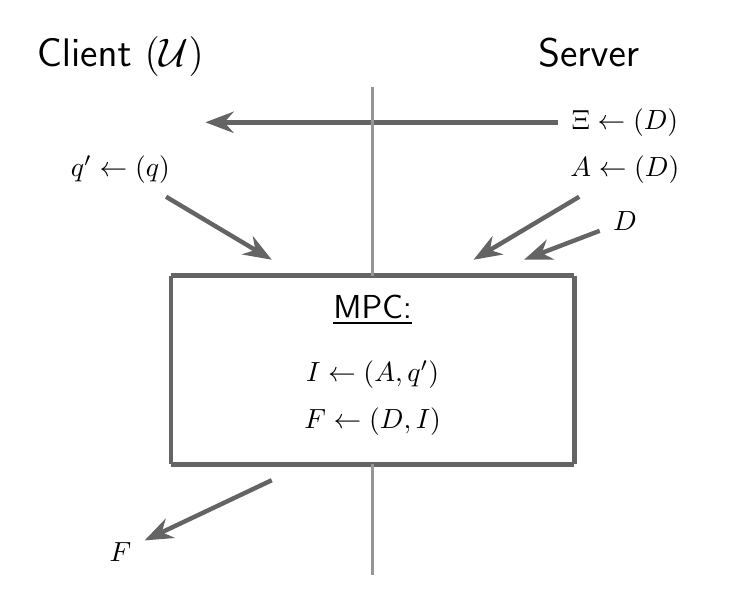
\begin{tikzpicture}[auto,>=Triangle,font=\sffamily]
        \node (server) {\Large Server $ \phantom{\left( \mathcal{U} \right)} $ };
        \node[base left=4cm  of server] (client) {\Large Client $ \left( \mathcal{U} \right) $};
        \coordinate[below=8cm of server] (server_ground);
        \coordinate[below=8cm of client] (client_ground);
        
        \begin{scope}[line width=3pt,shift={(client_ground)},
            nodes={above}, draw=dark_gray, x={($(server_ground)-(client_ground)$)},y={($(client.south)-(client_ground)$)}]
            \draw[] (1, 0.9) node (setup) {$ \Xi \gets \Setup \left( D \right) $};
            \draw[] (0.1, 0.9) node (setup_receive) {\phantom{$ \left( A \right) $}};
            \draw[ultra thick, -{Stealth[scale=1]}] (setup) -- (setup_receive);

            \draw[] (1, 0.825) node (filter) {$ A \gets \Filter \left( D \right) $};
            \draw[ultra thick, -{Stealth[scale=1]}] (filter) -- (0.7, 0.725);
            \draw[] (1, 0.75) node (filter) {$ D $};
            \draw[ultra thick, -{Stealth[scale=1]}] (filter) -- (0.8, 0.725);
            \draw[] (0, 0.825) node (q) { $ q' \gets \Hash \left( q \right) $};
            \draw[ultra thick, -{Stealth[scale=1]}] (q) -- (0.3, 0.725);

            \draw[ultra thick, -] (0.1, 0.7) -- (0.9, 0.7);
            \draw[ultra thick, -] (0.1, 0.7) -- (0.1, 0.4);
            \draw[ultra thick, -] (0.9, 0.7) -- (0.9, 0.4);
            \draw[ultra thick, -] (0.1, 0.4) -- (0.9, 0.4);

            \draw[] (0.5, 0.6) node (search) {\large \underline{MPC:}};

            \draw[] (0.5, 0.5) node (search) {$ I \gets \Search \left( A, q' \right) $};

            \draw[] (0.5, 0.425) node (retrieve) {$ F \gets \Retrieve \left( D, I \right) $};

            \draw[] (0, 0.225) node (decode) {$ F $};
            \draw[ultra thick, -{Stealth[scale=1]}] (0.3, 0.375) -- (decode);

            \draw[line width=1pt, light_gray] (0.5, 1) -- (0.5, 0.7);
            \draw[line width=1pt, light_gray] (0.5, 0.4) -- (0.5, 0.225);
        \end{scope}
    \end{tikzpicture}
    \captionsetup{justification=centering,margin=1cm}
    \caption{The proof of concept protocol's communication flow between the client and the server.}
\end{figure}

\refstepcounter{subsection}\subsection*{\thesubsection\quad Search}\label{subsec:ProofOfConceptSearching}


We must derive some auxiliary information $ A $ about the database in order to search it; therefore, $ A $ takes the form of an indexing. $ R^{\mathrm{values}}_{\iota} $ denote an array of the values in a specific record $ R_{\iota} $. Currently, the values in each record can be whatever, so we want a way to describe them in a standard format. A simple way to fingerprint a value is to produce its hash digest, so that is what we do, and we store the digests in $ A $.

\RestyleAlgo{ruled}
\begin{algorithm}[tbh]
    \LinesNumbered
    \caption{Proof of Concept - $ \Filter $}
    \label{algo:Indexing}
    \KwIn{Database $ D = \left[
            R^{\mathrm{values}}_1, 
            R^{\mathrm{values}}_2, 
            ... , 
            R^{\mathrm{values}}_m
        \right]  $}
    \KwOut{Indexing of the database \newline $ A = \left[ 
            R^{\mathrm{digests}}_1,
            R^{\mathrm{digests}}_2,
            ... ,
            R^{\mathrm{digests}}_m
        \right] $}

    \vspace*{0.48cm}

    {$ A \gets \lbrack \phantom{=} \rbrack $}

    \For {$ R^{\mathrm{values}}_{\iota} \mathrm{\phantom{|} in \phantom{|}} D $ } { 

        {$ R^{\mathrm{digests}}_{\iota} \gets \left[ \phantom{=} \right] $}

        \For {$ v_j \mathrm{\phantom{|} in \phantom{|}} R^{\mathrm{values}}_{\iota} $} {
            { $ R^{\mathrm{digests}}_{\iota} $.append$\left( \Hash{\left( v_j \right)}\right)$}
        }

        {$ A $.append$\left( R^{\mathrm{digests}}_{\iota} \right)$ }
    }

    \vspace*{0.48cm}

    \KwRet{$ A $}
\end{algorithm}

The only part remaining in the setup of the inputs is to encode the client's search query $ q $. Similarly to encoding the values, we create a digest of the search query, allowing us to match it with the digests in $ A $.

\RestyleAlgo{ruled}
\begin{algorithm}[tbh]
    \LinesNumbered
    \caption{Proof of concept - Encoding $ q $}
    \label{algo:EncodingTheSearchQuery}
    \KwIn{Search query $ q $}
    \KwOut{Encoded search query $ q' $}

    \vspace*{0.48cm}

    {$ q' \gets \Hash{(q)} $}

    \vspace*{0.48cm}

    \KwRet{$ q' $}
\end{algorithm}

We compute $ \Search $ using generic \acrshort{mpc}, meaning the client provides $ q' $ and the server $ A $ without revealing their input to the other party.  $ \Search $ outputs a set of indices $ I $ which is revealed to the client. The type of search we want to perform is a keyword search. To do this, we check if $ q' $ matches any digests in $ A $. If it does so, we store the index in $ I $.

\RestyleAlgo{ruled}
\begin{algorithm}[tbh]
    \LinesNumbered
    \caption{Proof of Concept - $ \Search $}
    \label{algo:Searching}
    \KwIn{Encoded search query $ q' $}
    \KwIn{Encoded indexing \newline $ A \gets \left[ 
            R^{\mathrm{digests}}_1,
            R^{\mathrm{digests}}_2,
            ... ,
            R^{\mathrm{digests}}_m
        \right] $}
    \KwOut{Indices $ I $}

    \vspace*{0.48cm}

    {$ I \gets \lbrack \phantom{=} \rbrack $}

    \For {$ R^{\mathrm{digests}}_{\iota} \mathrm{\phantom{|} in \phantom{|}} A $} {

        \For {$ digest \mathrm{\phantom{|} in \phantom{|}} R^{\mathrm{digests}}_{\iota} $} {
            \If {$ \left( q' = digest \right) \mathrm{\phantom{|} and \phantom{|}} \left( digest \mathrm{\phantom{|} not \phantom{|} in \phantom{|}}  I \right) $} {
                $ I $.append$\left(i\right)$
            }
        }
    }

    \vspace*{0.48cm}

    \KwRet{$ I $}
\end{algorithm}

\refstepcounter{subsection}\subsection*{\thesubsection\quad Retrieval}\label{subsec:ProofOfConceptRetrieval}


The second step is to retrieve the records for the indices $ I $ that the client learned in the search. We consider the database $ D $ to have the records as an array of characters, $ D = \left[ R^{\mathrm{chars}}_1, R^{\mathrm{chars}}_2, ... , R^{\mathrm{chars}}_m \right] $. Implicitly, the order of the records in the database is the same as in the search. To retrieve the records, we only take the records with an index in $ I $ and add them to the retrieved records at $ F $.

\RestyleAlgo{ruled}
\begin{algorithm}[tbh]
    \LinesNumbered
    \caption{Proof of concept - $ \Retrieve $}
    \label{algo:Retrieval}
    \KwIn{Indices $ I $}
    \KwIn{Database $ D \gets \left[
            R^{\mathrm{chars}}_1, 
            R^{\mathrm{chars}}_2, 
            ... , 
            R^{\mathrm{chars}}_m
        \right]  $}
    \KwOut{Retrieved records $ F $}

    \vspace*{0.48cm}

    $ F \gets \left[ \phantom{=}\right] $

    \For {$ i \in \lbrace 1, 2, ... , m \rbrace $} {
        \If {$ i $ in $ I $} {
            $ F $.append$ \left(R^{\mathrm{chars}}_{\iota}\right) $
        }
    }

    \vspace*{0.48cm}

    \KwRet{$ F $}
\end{algorithm}


\section{Results}
\label{sec:proofofconceptResults}
%\addcontentsline{toc}{section}{Results}

We now have the completed protocol, so let us implement it and perform some experiments. The experiment aims to determine which of MP-SPDZ's programs, i.e., generic \acrshort{mpc} protocols, yield the most efficient execution. We only test the ones that match our modeling, dishonest majority with semi-honest adversaries in the two-party setting. Given the data we get from the experiments, we discuss a way of better describing the efficiency of this protocol. Lastly, we discuss important considerations that the extracted metric from the experiments do not directly reflect.

\newcommand{\BigO}{\ensuremath{\mathsf{{O}}}}
The realization of the program deviates from the pseudocode's mid-level abstraction as we cannot branch, use dynamic data structures or index on hidden values. An algorithm for the solution implemented in MP-SPDZ is located in Appendix \hyperref[apx:proofofconceptSearchRetrieve]{B}. Among the more significant differences is that the indexing $ A $ is padded such that all the arrays of digests are the same length $ \sigma $. Secondly, the database $ D $, consisting of the records as characters, was padded such that all the arrays were of length $ \omega = 6016 $. We chose $ \omega $ as the maximum length any \acrshort{pnr} could have, which introduces significant redundancy, making the average record two to three times larger. The computational complexity for $ \Search $ ended up being $ \BigO \left( m \cdot \sigma \right) $, and for $ \Retrieve $ it is $ \mathcal{O} \left( m \cdot \omega \right) $. This amortization alone does not answer the question of feasibility, so let us discuss the data from the experiments.

We combine \cref{algo:Searching} ($ \Search $) and \cref{algo:Retrieval} ($ \Retrieve $) into one implementation as the results $ I $ from $ \Search $ can be directly passed to $ \Retrieve $. This means that we produce and supply $ A $, $ q' $, and $ D $ into MP-SPDZ simultaneously. Respectively, the server runs \cref{algo:Indexing} ($ \Filter $), and the client runs \cref{algo:EncodingTheSearchQuery} (search query encoding). Together they execute the combination of \cref{algo:Searching} ($ \Search $) and \cref{algo:Retrieval} ($ \Retrieve $). We instantiate $ \Hash $ as SHA256.

\begin{figure} [tbh]
    \caption{Proof of Concept - Runtimes}
    \label{fig:ProofOfConceptRuntimes}
    \centering
    \begin{tikzpicture}
        \begin{axis}[
            xlabel={Number of Records $ m $},
            ylabel={seconds},
            grid=major,
            cycle list name=black white,
            legend entries={semi-party.x, hemi-party.x, temi-party.x, soho-party.x},
            legend pos=outer north east
        ]
        

        \addplot table {../Chapter Proof of Concept/Data/semi_party.txt};
        \addplot table {../Chapter Proof of Concept/Data/hemi_party.txt};
        \addplot table {../Chapter Proof of Concept/Data/temi_party.txt};
        \addplot table {../Chapter Proof of Concept/Data/soho_party.txt};
        \end{axis}
    \end{tikzpicture}
\end{figure}

For this program, we are only interested in the runtime of the algorithms implemented using generic \acrshort{mpc}. MP-SPDZ provides us with a few different programs to test with, and of course, we want to figure out which of these provides us with the fastest execution. We take the benchmark metrics directly from MP-SPDZ as our results, but only consider programs that offer security for a dishonest majority with semi-honest adversaries. With the results, we are only concerned with the magnitude of the runtime; hence, a single execution suffices.

The results, \cref{fig:ProofOfConceptRuntimes} and \cref{Tab: Proof of Concept benchmarking}, show that semi-party.x yields the fastest runtime. It can perform a search query on one hundred records in 36.5 seconds, which might seem promising initially, but the number of records alone is an imprecise metric. A better metric for discussing the feasibility is to talk about the total byte size of the database. That is the number of records multiplied by the size of the records. For simplicity and to better communicate the actual throughput of the program, we use the size of the padded records. Hence, $ m * \omega $ is how we calculate the total size. The use of $ \omega $  abstracts away the redundant data added by padding the records, which separates the problem of how to efficiently pad the records into a separate discussion. Performing the calculation $ m * \omega = 100 \cdot 6016 $ (one character is one byte) gives us a database size of 601.6 kilobytes. Scaling this up, we find that we can perform a single search query in time budget $ \tau = $ eight hours on a database of size 300 megabytes. An interesting observation is that MP-SPDZ provides the total communication costs for the execution. We find that the difference between the inputs we provide to MP-SPDZ and the total communication costs is more than a factor of a hundred. This high communication cost comes from the additional communication required to compute, in our case, many multiplication operations.

Apart from the runtime, there are valuable considerations that the data above does not reflect: 1) The MP-SPDZ part of the program has to be recompiled before each execution as the number of values in the records, $ \sigma $, varies depending on the records in the database. A solution would be to choose $ \sigma $ as the maximum possible number of values a record could have, but this would introduce even more redundant data. 2) We observe that the inability to have dynamic storage structures, indexing on secret values, and branching forces us to develop a solution that does more work than ideal. For example, we have to structure our data to skip a loop in \cref{algo:RetrieveAndSearch} ($ \Search $ \& $ \Retrieve $) since we cannot index on secret values. Furthermore, we also have to loop over the whole array of $ I $ of length $ m $ instead of dynamically being able to append non-zero indices to it. \footnote{A set-like data structure and a dynamic array can be achieved using \acrshort{oram} in MP-SPDZ, but from testing, these solutions yield much worse results in terms of runtime.}

\begin{center}
    \begin{table} [tbh]
        \centering
        \begin{threeparttable}
            \caption{Proof of Concept - Benchmarking}
            \label{Tab: Proof of Concept benchmarking}
            \begin{tabular}{|c | c | c | c|} 
            \hline
            Program & Number of Records ($ m $) & Runtime (\si{\second}) & Total comm. (\si{\mega\byte}) \\ [0.5ex] 
            \hline\hline
            \multirow{3}{4em}{semi-party.x} & 1 & 0.336 & 0.67 \\
             & 10 & 3.646 & 7.29 \\
             & 100 & 36.538 & 73.08 \\ [3ex] 
            \multirow{3}{4em}{hemi-party.x} & 1 & 2.036 & 4.07 \\
             & 10 & 17.3 & 34.6 \\
             & 100 & 173.462 & 346.92 \\ [3ex] 
            \multirow{3}{4em}{temi-party.x} & 1 & 2.941 & 5.88 \\
             & 10 & 22.787 & 45.57 \\
             & 100 & 227.216 & 454.43 \\ [3ex] 
            \multirow{3}{4em}{soho-party.x}& 1 & 13.914 & 27.38 \\
             & 10 & 51.346 & 102.69 \\
             & 100 & 557.26 & 1114.52 \\
            [1ex]
            \hline
            \end{tabular}
            \begin{tablenotes}
                \small
                \item \si{\second} denotes seconds, \si{\mega\byte} denoted megabytes, comm. denotes communcation.
            \end{tablenotes}
        \end{threeparttable}
    \end{table}
\end{center}

To summarize, the proof of concept indicates that supporting a reasonably large database is possible. However, the constraints introduced by structuring the whole protocol in generic \acrshort{mpc} limit its efficiency.

\section{Security}
\label{sec:proofofconceptSecurity}
%\addcontentsline{toc}{section}{Security}

Recall that we implemented $ \Search $ and $ \Retrieve $ as a program in MP-SPDZ. Therefore, security boils down to the security of the underlying generic \acrshort{mpc} protocol, its implementation in MP-SPDZ, and the overall security of MP-SPDZ. These things are subject to change and are, therefore, out of the scope of this work. Instead, let us talk about the deviations from the desired functionality and additional risks not captured by it. We relate the program to our notion of privacy, discuss the information leakage in our program and finish with a discussion on an important practical implication, namely false positives, and propose mitigations to it.  

For security, we want to protect against semi-honest adversaries. We are only concerned with a client and a server, so only two parties are involved, which means that if either party is dishonest, any protocol that assumes an honest majority is not sufficient. To model our parties, we instantiate them as an independent process whose only communication is through the interface MP-SPDZ. The only values that the client sees are $ q $ and $ F $, and the server only sees $ A $ and $ D $. We assume that the underlying generic \acrshort{mpc} protocol provides semantic security, our privacy notion holds as the server does learn anything about the query and the result, while the client only learns the result.

\refstepcounter{subsection}\subsection*{\thesubsection\quad Information Leakage}\label{subsec:ProofOfConceptInformationLeakage}


Regarding the program's output, it is not enough to consider the actual values revealed as the only information revealed to the client, as context and structure could also leak unwanted information. Here, we exclude all information in the records from the assessment and side channel leaks.

There is only one output of the program, which is revealed to the client. That output $ F $ has the same structure as the database input from the server, so it leaks the following information: 1) How many records, $ m $, there are since the number of rows it has is directly correlated to $ m $. A simple solution to avoid this is to pad the database to a fixed length. However, this would be costly in terms of adding redundant computations while being ineffective, as the magnitude of the number of records is still revealed. 2) The indices of the retrieved records. These can be used to deduce further information. For example, combining results from multiple searches can be used to infer deletion and creation of new records. A solution to avoid this is by shuffling the order in which the records are read. 3) The value of $ \omega $, which is intrinsic to the program's description.

\refstepcounter{subsection}\subsection*{\thesubsection\quad False Positives}\label{subsec:False Positives}

In the computation, we define a matching of the search query and a record if the digest of the search query is equal to the digest of one of the values in the record. It follows from using a cryptographically secure hash function that we do not get false positives in this matching, so that is not a concern, but what is a concern is the input-space to the hash function, as many of the values in the record have a small range. For example, the set of phone numbers, excluding prefixes, is small. This small input space could lead to false positives. An even better example is that some people have the same names. A solution to mitigate this weakness is for the server to filter keys and values when creating the indexing of the records, so the client has to provide sufficient evidence to satisfy the search criteria. A potential solution is to extend the search to allow the client to provide a set of inputs for the search query, which is combined to determine if the client has provided sufficient evidence. Like a scoring system, where a positive match to some values in the records is worth more than others, and in the end, the amount of information the client receive depends on the accumulated score.


\chapter{Private Database Search Protocol}
\label{chap:SolutionPDS}
%\addcontentsline{toc}{chapter}{Oblivious Private Database Search}

\acrshort{pds} is realized by combining \acrshort{psi} and \acrshort{ot}. Therefore, to create a scheme, we propose two \acrshort{psi} protocols where one provides a keyword search functionality and the other a semantic search functionality, and an \acrshort{ot} protocol that allows the client to retrieve records from the database. These protocols interoperate, so to give a clear picture, we start by giving an overview of the communication flow between the client and server. Then, we introduce the \acrshort{ot} protocol in two sections: one that describes the initiation phase and one for the transfer phase. We also separate the \acrshort{psi} protocols into an initiation and a transfer phase. To answer the question of feasibility, we perform experiments that implement the proposed protocols. Lastly, we discuss the results, in the context of the descriptions we gave for the properties of \acrshort{pds}, the practicability and post-quantum security of the proposed protocol.
\section{Protocol Overview}
\label{sec:protocoloverview}
%\addcontentsline{toc}{section}{Protocol Overview}

\newcommand{\PreProcess}{\ensuremath{\mathsf{{PreProcess}}}}
\newcommand{\Encrypt}{\ensuremath{\mathsf{{Encrypt}}}}
\newcommand{\Permute}{\ensuremath{\mathsf{{Permute}}}}
\newcommand{\Sort}{\ensuremath{\mathsf{{Sort}}}}
\newcommand{\Decrypt}{\ensuremath{\mathsf{{Decrypt}}}}
\newcommand{\Distance}{\ensuremath{\mathsf{{Distance}}}}
\newcommand{\KeyGen}{\ensuremath{\mathsf{{KeyGen}}}}
The general idea is to present solutions to the five algorithms $ \Filter $, $ \Search $, $ \Encode $, $ \Retrieve $ and $ \Decode $ such that they satisfy our description of privacy, correctness, adaptive, storage imbalance, access control and timely. \cref{fig:CommunicationFlow} outlines, but does not limit, the communication flow between the client and server in the five algorithms, therefore we introduce additional algorithms to realize the protocol.

We do not focus on the $ \Setup $ algorithm, but we highlight that $ \Setup $ shuffles the order of the records on the database. Recall that \acrshort{pds} consists of a \acrshort{psi} protocol, to facilitate the search, combined with an \acrshort{ot} protocol, to facilitate the retrieval. We propose two \acrshort{psi} protocols that provide the functionality of a keyword search and semantic search on the database, and one \acrshort{ot} protocol that allows retrieval of records from the database. However, the two types of searches are independently realized so a \acrshort{pds} protocol might only include one, therefore, we present both as their own stand-alone protocol. Overall, the protocol is split into an initiation step of the subprotocols and a transfer step where the protocol is executed. To realize the protocol we extend the work in \cref{chap:PDS} and introduce eight new algorithms and re-introduce $ \Garble $:

\begin{description}
    \item[$ \PreProcess $] takes in the database $ D $, and outputs the set of dummy item indices $ \eta $, a permutation $ \pi \subseteq {\lbrace 1, 2, ... , n \rbrace} $ of length $ n $, encryption keys $ K $, and the encoded database $ D' $ with the files encrypted and shuffled.
    \item[$ \Encrypt $] takes in a plaintext and encryption key of length $ \beta $, and outputs a ciphertext of length $ \beta $.
    \item[$ \Garble $] takes in some auxiliary information $ A $, and outputs the encrypted auxiliary information $ A' $.
    \item[$ \Permute $] takes in an array, and outputs a permutation $ \pi $ of that array.
    \item[$ \Sort $] takes in a permutation $ \pi $, and outputs a series of indices $ i, j $ and a bit $ b $ that indicates whether the indices should be swapped or not.
    \item[$ \Hash $] takes in some binary string and outputs a digest of length $ \beta $.
    \item[$ \Decrypt $] takes in a ciphertext and encryption key of length $ \beta $, and outputs a plaintext of length $ \beta $.
    \item[$ \Distance $] takes in two vectors and calculates the distance between them. 
    \item[$ \KeyGen $] takes in no input but outputs an encryption key and other variables like IVs, nonces and counters.
\end{description}

For the sake of brevity but without the lack of generality, we abstract some detailed functionalities into a general \acrshort{mpc} description to best communicate the overall idea behind the algorithms.
\refstepcounter{subsection}\subsection*{\thesubsection\quad Initiation}\label{subsec:OverviewInitiation}

The initiation intends to preprocess as much as possible before the transfers. In it, a couple of things happen, showcased by \cref{fig:OverviewPreProcess}. The server fills the database $ D $ with dummy records such that it is of length $ n $ and pads all its records to a fixed length. Once that is done, the $ \PreProcess $ algorithm encrypts the database under the client's keys $ K $ and sort it according to some random permutation $ \pi $ that the client gets by running $ \Permute $. $ \PreProcess $ achieves this by internally using $ \Sort $ and $ \Encrypt $. The idea is that the sorting is done obliviously to the server and that the encryption of the files is oblivious to the client, without the server learning $ K $ and the client learning the contents of $ D $. At the end, the server is left with the encoded database $ D' $ where it cannot correlate the ciphertexts in $ D' $ to the records in $ D $.

\begin{figure}[H]
    \centering
    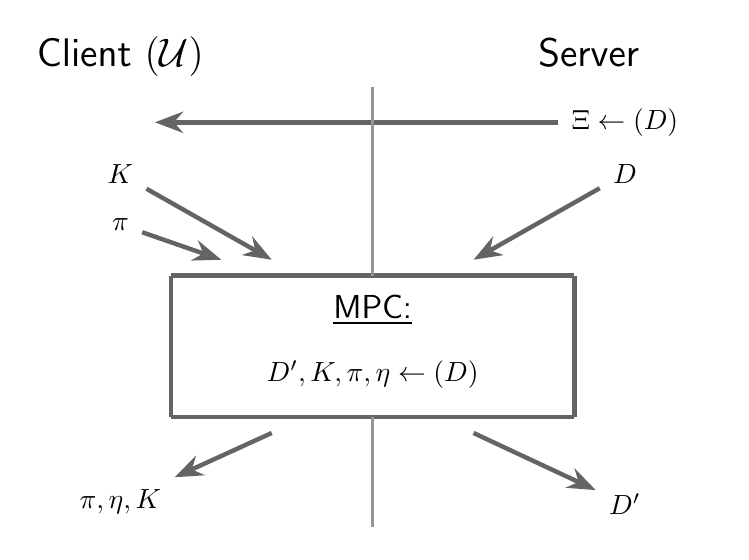
\begin{tikzpicture}[auto,>=Triangle,font=\sffamily]
        \node (server) {\Large Server $ \phantom{\left( \mathcal{U} \right)} $ };
        \node[base left=4cm  of server] (client) {\Large Client $ \left( \mathcal{U} \right) $};
        \coordinate[below=8cm of server] (server_ground);
        \coordinate[below=8cm of client] (client_ground);
        
        \begin{scope}[line width=3pt,shift={(client_ground)},
            nodes={above}, draw=dark_gray, x={($(server_ground)-(client_ground)$)},y={($(client.south)-(client_ground)$)}]
            \draw[] (1, 0.9) node (setup) {$ \Xi \gets \Setup \left( D \right) $};
            \draw[] (0, 0.9) node (setup_receive) {\phantom{$ \left( A \right) $}};
            \draw[ultra thick, -{Stealth[scale=1]}] (setup) -- (setup_receive);

            \draw[] (1, 0.825) node (filter) {$ D $};
            \draw[ultra thick, -{Stealth[scale=1]}] (filter) -- (0.7, 0.725);
            \draw[] (0, 0.75) node (filter) {$ \pi $};
            \draw[ultra thick, -{Stealth[scale=1]}] (filter) -- (0.2, 0.725);
            \draw[] (0, 0.825) node (q) { $ K $};
            \draw[ultra thick, -{Stealth[scale=1]}] (q) -- (0.3, 0.725);

            \draw[ultra thick, -] (0.1, 0.7) -- (0.9, 0.7);
            \draw[ultra thick, -] (0.1, 0.7) -- (0.1, 0.475);
            \draw[ultra thick, -] (0.9, 0.7) -- (0.9, 0.475);
            \draw[ultra thick, -] (0.1, 0.475) -- (0.9, 0.475);

            \draw[] (0.5, 0.6) node (search) {\large \underline{MPC:}};

            \draw[] (0.5, 0.5) node (search) {$ D', K, \pi, \eta \gets \PreProcess \left( D \right) $};

            \draw[] (1, 0.3) node (decode) {$ D' $};
            \draw[ultra thick, -{Stealth[scale=1]}] (0.7, 0.45) -- (decode);

            \draw[] (0, 0.3) node (decode) {$ \pi, \eta, K $};
            \draw[ultra thick, -{Stealth[scale=1]}] (0.3, 0.45) -- (decode);

            \draw[line width=1pt, light_gray] (0.5, 1) -- (0.5, 0.7);
            \draw[line width=1pt, light_gray] (0.5, 0.475) -- (0.5, 0.3);
        \end{scope}
    \end{tikzpicture}
    \captionsetup{justification=centering,margin=1cm}
    \caption{The communication flow between the client and the server in the database initiation (for clarity this overview is simplified).}
    \label{fig:OverviewPreProcess}
\end{figure}

Next we do more preprocessing to set up the two types of searches. In both types, the $ \Filter $ algorithm will be used to derive some auxiliary information $ A $ about the database, but the implementation of $ \Filter $ will differ. 

For the first type, keyword search, \cref{fig:OverviewInitKeywordSearch}, the server will create an indexing that is encrypted, using $ \Garble $, and then send it to the client. $ \Garble $ internally uses some implementation of $ \Encrypt $ and $ \Hash $ to encrypt elements. This encryption will happen with two keys, $ e_1 $ and $ e_2 $. To enforce the access control the server will filter values when creating the indexing, based upon the client's identity $ \mathcal{U} $. 

\begin{figure}[H]
    \centering
    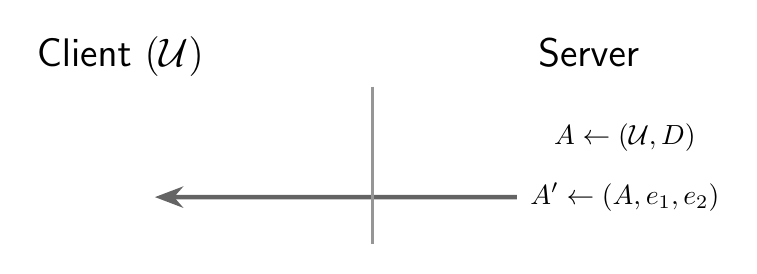
\begin{tikzpicture}[auto,>=Triangle,font=\sffamily]
        \node (server) {\Large Server $ \phantom{\left( \mathcal{U} \right)} $ };
        \node[base left=4cm  of server] (client) {\Large Client $ \left( \mathcal{U} \right) $};
        \coordinate[below=10cm of server] (server_ground);
        \coordinate[below=10cm of client] (client_ground);
        
        \begin{scope}[line width=3pt,shift={(client_ground)},
            nodes={above}, draw=dark_gray, x={($(server_ground)-(client_ground)$)},y={($(client.south)-(client_ground)$)}]
            \draw[] (1, 0.9) node (filter) {$ A \gets \Filter \left( \mathcal{U}, D \right) $};
            \draw[] (1, 0.825) node (garble) {$ A' \gets \Garble \left( A, e_1, e_2 \right) $};
            \draw[] (0, 0.825) node (garble_receive) {\phantom{$ \left( A \right) $}};
            \draw[ultra thick, -{Stealth[scale=1]}] (garble) -- (garble_receive);

            \draw[line width=1pt, light_gray] (0.5, 1) -- (0.5, 0.8);
        \end{scope}
    \end{tikzpicture}
    \captionsetup{justification=centering,margin=1cm}
    \caption{The communication flow between the client and the server in the keyword search initiation.}
    \label{fig:OverviewInitKeywordSearch}
\end{figure}

In the second type, semantic search, we use a \acrshort{llm}, denoted $ \Gamma $, to create vector embeddings of each record. These embeddings are stored with the corresponding index of the records. The access control is enforced by the server filtering information from the records before supplying it to $ \Gamma $, thereby only capturing the intended semantics in the vector embeddings.

\begin{figure}[H]
    \centering
    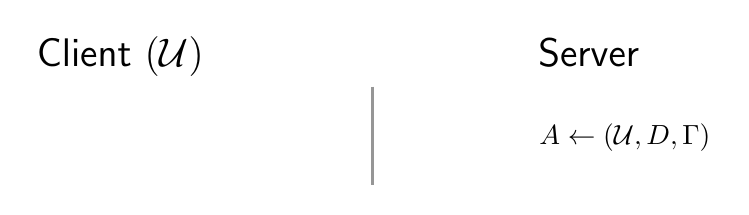
\begin{tikzpicture}[auto,>=Triangle,font=\sffamily]
        \node (server) {\Large Server $ \phantom{\left( \mathcal{U} \right)} $ };
        \node[base left=4cm  of server] (client) {\Large Client $ \left( \mathcal{U} \right) $};
        \coordinate[below=10cm of server] (server_ground);
        \coordinate[below=10cm of client] (client_ground);
        
        \begin{scope}[line width=3pt,shift={(client_ground)},
            nodes={above}, draw=dark_gray, x={($(server_ground)-(client_ground)$)},y={($(client.south)-(client_ground)$)}]
            \draw[] (1, 0.9) node (setup) {$ A \gets \Filter \left( \mathcal{U}, D, \Gamma \right) $};
            \draw[] (0.1, 0.9) node (setup_receive) {\phantom{$ \left( A \right) $}};

            \draw[line width=1pt, light_gray] (0.5, 1) -- (0.5, 0.875);
        \end{scope}
    \end{tikzpicture}
    \captionsetup{justification=centering,margin=1cm}
    \caption{The communication flow between the client and the server in semantic search initiation.}
    \label{fig:OverviewInitSemanticSearch}
\end{figure}
\refstepcounter{subsection}\subsection*{\thesubsection\quad Transfer}\label{subsec:OverviewTransfer}

The transfer step can be executed $ k $ number of times. We call an execution a transfer, as the server obliviously transfers files to the client. A transfer has the client and server perform the $ \Encode $, $ \Retrieve $, and $ \Decode $ algorithms in both the keyword search and semantic search variants, with the implementation of $ \Search $ differing between the two.

In the first type, keyword search, the client has the encrypted auxiliary information $ A' $ that we want it to compare with its search query $ q_i $. The way the client does this is by getting the hash $ q'_i $ of its search query, using the $ \Hash $ algorithm, encrypted with algorithm $ \Encrypt $ under the server's encryption keys $ e_1 $ and $ e_2 $ using generic \acrshort{mpc}. Once it has the two encrypted variants $ q_{i, e_1} $ and $ q_{i, e_2} $, it will use them with $ \Search $, which internally uses the $  \Decrypt$ algorithm, to derive a set of indices $ I_i $.

\begin{figure}[H]
    \centering
    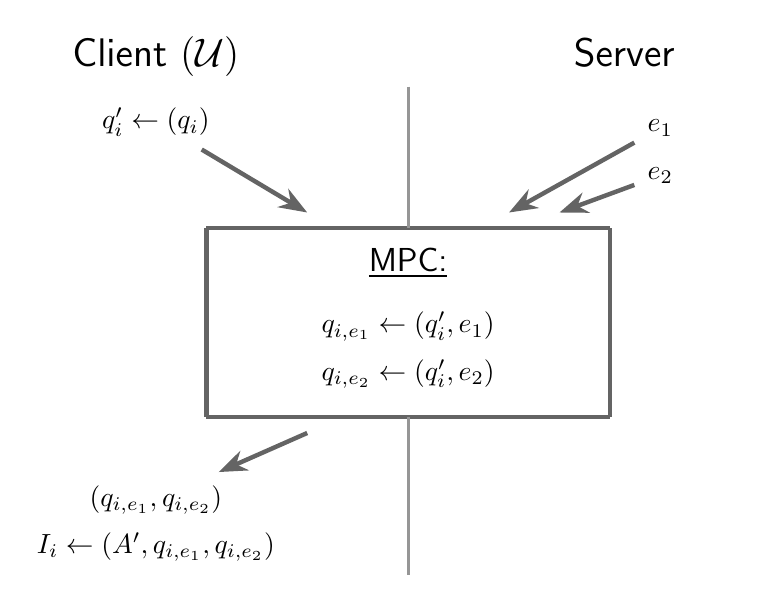
\begin{tikzpicture}[auto,>=Triangle,font=\sffamily]
        \node (server) {\Large Server $ \phantom{\left( \mathcal{U} \right)} $ };
        \node[base left=4cm  of server] (client) {\Large Client $ \left( \mathcal{U} \right) $};
        \coordinate[below=8cm of server] (server_ground);
        \coordinate[below=8cm of client] (client_ground);
        
        \begin{scope}[line width=3pt,shift={(client_ground)},
            nodes={above}, draw=dark_gray, x={($(server_ground)-(client_ground)$)},y={($(client.south)-(client_ground)$)}]

            \draw[] (1, 0.9) node (filter) {$ e_1 $};
            \draw[ultra thick, -{Stealth[scale=1]}] (filter) -- (0.7, 0.8);
            \draw[] (1, 0.825) node (filter) {$ e_2 $};
            \draw[ultra thick, -{Stealth[scale=1]}] (filter) -- (0.8, 0.8);
            \draw[] (0, 0.9) node (q) { $ q'_i \gets \Hash \left( q_i \right) $};
            \draw[ultra thick, -{Stealth[scale=1]}] (q) -- (0.3, 0.8);

            \draw[ultra thick, -] (0.1, 0.775) -- (0.9, 0.775);
            \draw[ultra thick, -] (0.1, 0.775) -- (0.1, 0.475);
            \draw[ultra thick, -] (0.9, 0.775) -- (0.9, 0.475);
            \draw[ultra thick, -] (0.1, 0.475) -- (0.9, 0.475);

            \draw[] (0.5, 0.675) node {\large \underline{MPC:}};

            \draw[] (0.5, 0.575) node (encrypt1) {$ q_{i, e_1} \gets \Encrypt \left( q'_i, e_1 \right) $};
            \draw[] (0.5, 0.5) node (encrypt2) {$ q_{i, e_2} \gets \Encrypt \left( q'_i, e_2 \right) $};

            \draw[] (0, 0.3) node (q) {$ \left( q_{i, e_1}, q_{i, e_2} \right) $};
            \draw[ultra thick, -{Stealth[scale=1]}] (0.3, 0.45) -- (q);

            \draw[] (0, 0.225) node (search) {$ I_i \gets \Search \left( A', q_{i, e_1}, q_{i, e_2} \right) $};


            \draw[line width=1pt, light_gray] (0.5, 1) -- (0.5, 0.775);
            \draw[line width=1pt, light_gray] (0.5, 0.475) -- (0.5, 0.225);
        \end{scope}
    \end{tikzpicture}
    \captionsetup{justification=centering,margin=1cm}
    \caption{The communication flow between the client and the server in the keyword search transfer.}
    \label{fig:OverviewTransferKeywordSearch}
\end{figure}

In the second type, semantic search, the client will use $ \Gamma $ to construct a vector embedding $ q_i' $ of its search query $ q_i $. $ \Search $ will be performed with the client inputting $ q_i' $ and the server inputting $ A $ to a generic \acrshort{mpc} protocol that compares $ q'_i $ and $ A $ using $ \Distance $. The output of $ \Search $ is a set of indices $ I_i $. 

\begin{figure}[H]
    \centering
    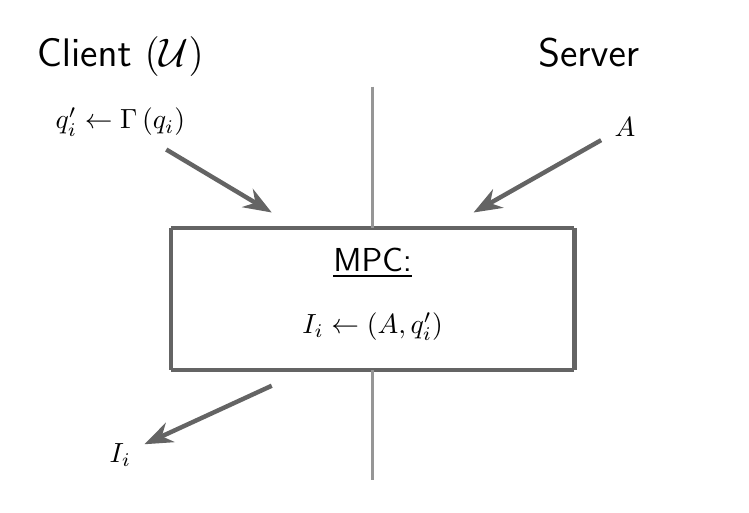
\begin{tikzpicture}[auto,>=Triangle,font=\sffamily]
        \node (server) {\Large Server $ \phantom{\left( \mathcal{U} \right)} $ };
        \node[base left=4cm  of server] (client) {\Large Client $ \left( \mathcal{U} \right) $};
        \coordinate[below=8cm of server] (server_ground);
        \coordinate[below=8cm of client] (client_ground);
        
        \begin{scope}[line width=3pt,shift={(client_ground)},
            nodes={above}, draw=dark_gray, x={($(server_ground)-(client_ground)$)},y={($(client.south)-(client_ground)$)}]

            \draw[] (1, 0.9) node (filter) {$ A $};
            \draw[ultra thick, -{Stealth[scale=1]}] (filter) -- (0.7, 0.8);
            \draw[] (0, 0.9) node (q) { $ q'_i \gets \Gamma \left( q_i \right) $};
            \draw[ultra thick, -{Stealth[scale=1]}] (q) -- (0.3, 0.8);

            \draw[ultra thick, -] (0.1, 0.775) -- (0.9, 0.775);
            \draw[ultra thick, -] (0.1, 0.775) -- (0.1, 0.55);
            \draw[ultra thick, -] (0.9, 0.775) -- (0.9, 0.55);
            \draw[ultra thick, -] (0.1, 0.55) -- (0.9, 0.55);

            \draw[] (0.5, 0.675) node {\large \underline{MPC:}};

            \draw[] (0.5, 0.575) node (encrypt1) {$ I_i \gets \Search \left( A, q'_i \right) $};

            \draw[] (0, 0.375) node (q) {$ I_i $};
            \draw[ultra thick, -{Stealth[scale=1]}] (0.3, 0.525) -- (q);

            \draw[line width=1pt, light_gray] (0.5, 1) -- (0.5, 0.775);
            \draw[line width=1pt, light_gray] (0.5, 0.55) -- (0.5, 0.375);
        \end{scope}
    \end{tikzpicture}
    \captionsetup{justification=centering,margin=1cm}
    \caption{The communication flow between the client and the server in the semantic search transfer.}
    \label{fig:OverviewTransferSemanticSearch}
\end{figure}

Recall that we created the encoded database $ D' $ by sorting  datbase according to the random permutation $ \pi $. To retrieve the records, the client uses $ \pi $ to encode the indices $ I'_i $ and then sends them to the server. The server, in possession of $ D' $, responds with the encrypted records $ F'_i $, which the client decrypts with the keys $ K $ to derive the set of records $ F_i $ for that transfer.

\begin{figure}[H]
    \centering
    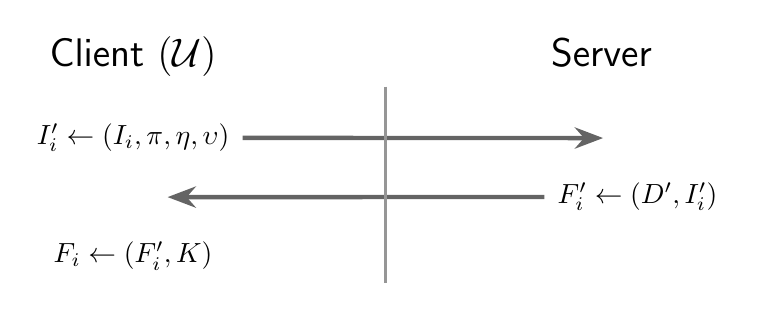
\begin{tikzpicture}[auto,>=Triangle,font=\sffamily]
        \node (server) {\Large Server $ \phantom{\left( \mathcal{U} \right)} $ };
        \node[base left=4cm  of server] (client) {\Large Client $ \left( \mathcal{U} \right) $};
        \coordinate[below=10cm of server] (server_ground);
        \coordinate[below=10cm of client] (client_ground);
        
        \begin{scope}[line width=3pt,shift={(client_ground)},
            nodes={above}, draw=dark_gray, x={($(server_ground)-(client_ground)$)},y={($(client.south)-(client_ground)$)}]
            \draw[] (0, 0.9) node (setup) {$ I'_i \gets \Encode \left( I_i, \pi, \eta, \upsilon \right) $};
            \draw[] (1, 0.9) node (setup_receive) {\phantom{$ \left( A \right) $}};
            \draw[ultra thick, -{Stealth[scale=1]}] (setup) -- (setup_receive);
            \draw[] (1, 0.825) node (filter) {$ F'_i \gets \Retrieve \left( D', I'_i\right) $};
            \draw[] (0, 0.825) node (filter_receive) {\phantom{$ \left( A \right) $}};
            \draw[ultra thick, -{Stealth[scale=1]}] (filter) -- (filter_receive);
            \draw[] (0, 0.75) node (filter) {$ F_i \gets \Decode \left( F'_i, K \right) $};

            \draw[line width=1pt, light_gray] (0.5, 1) -- (0.5, 0.75);
        \end{scope}
    \end{tikzpicture}
    \captionsetup{justification=centering,margin=1cm}
    \caption{The communication flow between the client and the server in the file retrieval.}
    \label{fig:OverviewRetrieve}
\end{figure}

\section{Database Initiation}
\label{sec:databaseinitiation}
%\addcontentsline{toc}{section}{Transfer initiation}

From the proof of concept, we found that for a megabyte-sized database, it takes hours to complete a single transfer, therefore, it would be beneficial to structure our protocol so that we do most of the costly work in advance. We encode our database $ D $ in the initiation to make the transfers as efficient as possible. The overarching idea is for the client to obliviously encrypt and shuffle $ D $ with its keys $ K $ and permutation $ \pi $. If we were to follow a general \acrshort{oram} construction, the client would non-obliviously encrypt the records and use an oblivious sorting algorithm to shuffle them. This process would only provide privacy in one way; hence, we introduce the notion of \acrfull{ps}, which yields privacy for both the client and server in the shuffling and encryption of the database. For \acrshort{ps}, we present an efficient generic \acrshort{mpc} protocol that uses binary circuits. We use a generic \acrshort{mpc}-based \acrshort{ps} protocol in combination with an oblivious sorting algorithm to implement the $ \PreProcess $ algorithm. With the implementation, we perform experiments to find the largest database size we can support within a time budget $ \tau $ of eight hours. After presenting the results from the experiment, we propose an \acrshort{ot}-based \acrshort{ps} protocol and discuss its potential efficiency.
\newcommand{\CTR}{\ensuremath{\mathsf{{CTR}}}}
\refstepcounter{subsection}\subsection*{\thesubsection\quad The $ \PreProcess $ algorithm}\label{subsec:PreProcessAlgorithm}

To pad each record is important as the length of a record could work as a direct identifier even if it is encrypted. We use the same idea as in the proof of concept to pad the records; we settle for an upper bound $ \omega $, which is the maximal length of any possible record $ R^{\mathrm{chars}}_{\iota} $. We then pad all records such that they are of length $ \omega $. Later in the transfer step, we must make valid retrievals of "empty" records, therefore, we fill the database with dummy records $ d_i $ of length $ \omega $. We add the dummy records after the records such that the database from index $ 1 $ to $ m $ consists of records $ R_{\iota} $, and from $ m + 1 $ to $ n $ consists of dummy records. The number of dummy records added will later determine how many transfers $ k $ can be made. This way of adding the dummy records allows the client to infer their location implicitly by the server sending it the length of the database $ n $ and the number of records $ m $.

\hfill

\RestyleAlgo{ruled}
\begin{algorithm}[H]
    \LinesNumbered
    \caption{Server - Padding the Database}
    \label{algo:DatabasePadding}
    \KwIn{Database $ D \gets \left[
            R^{\mathrm{chars}}_1, 
            R^{\mathrm{chars}}_2, 
            ... , 
            R^{\mathrm{chars}}_m
        \right]  $}
    \KwOut{Database $ D' \gets \left[
        R'_1, 
        R'_2, 
        ... , 
        R'_m,
        d_1,
        d_2,
        ... ,
        d_{n - m}
    \right]  $}

    \vspace*{0.48cm}

    $ D' \gets \left[ \phantom{=}\right] $

    \For{$ R^{\mathrm{chars}}_{\iota} \mathrm{\phantom{|} in \phantom{|}} D $}{
        
        $ R'_i \gets R^{\mathrm{chars}}_{\iota} $.padToLength$ \left(\omega\right)$

        $ D' $.append$\left( R'_i \right)$

    }

    \For {$ i \in \lbrace 1, 2, ... , n - m \rbrace $} {
        
        $ D' $.append$ \left( d_i \right) $

    }

    \vspace*{0.48cm}

    \KwRet{$ D' $}
\end{algorithm}

\clearpage

We now have a database with records and dummy records that the client wants to shuffle. The client uses an oblivious sort algorithm $ \Sort $ to sort the database $ D' $ after some random permutation $ \pi $ of length $ n $. For simplicity, we say that the sorting algorithm considers two and two records at a time, denote with $ i, j, b \gets \Sort $, where $ i, j \in \lbrace 1, 2, ... , n \rbrace $ are indices of the records and $ b \in \lbrace 0, 1 \rbrace $ is a bit to signal whether to swap or not. The challenge is how the client can request records $ R_i $ and $ R_j $, encrypting and potentially swap them without learning the records. This might seem like a simple problem at first, as the server could mask the records before sending them away, but how is the server supposed to unmask them without the client revealing which mask goes with which record? In this sense, we need an oblivious swapping algorithm combined with two-way masking of the records, which brings us to the notion of private swap.

\hfill

\noindent
\begin{figure}[H]
    \begin{minipage}{0.5\textwidth}
        \RestyleAlgo{ruled}
        \begin{algorithm}[H]
            \LinesNumbered
            \caption{Client $ \mathcal{U} $ - \newline $ \PreProcess $}
            \label{algo:ClientPreProcess}
            \KwIn{\phantom{$ D' $}}
            
            \vspace*{0.48cm}
    
            \KwOut{Permutation $ \pi $}
            \KwOut{Dummy indices $ \eta $}
            \KwOut{Keys $ K $}
    
            \vspace*{0.48cm}
    
            $ K \gets \left[ \phantom{=} \right] $ 
    
            receive $ \left(m, n\right) $
    
            $ \eta \gets \left[ m + 1, m + 2, ... , n \right] $
        
            $ \pi \gets \Permute \left( \left[ 1, 2, ... , n \right] \right) $
    
            \For{$ i, j, b \mathrm{\phantom{|} in \phantom{|}} \Sort \left( \pi \right) $}{
                
                send $ \left( i, j \right) $
    
                \SetKwProg{PS}{private swap:}{}{end}
                \PS{}{
    
                    \KwIn{$ K, i, j, b $ \phantom{$ D'_i, D'_j $}}
    
                    \KwOut{\phantom{$ C_i, C_j $}}
    
                }
    
                \phantom{$ D'_i $}
    
                \phantom{$ D'_j $}
            }
    
            \vspace*{0.48cm}
        
            \KwRet{$ \pi, \eta, K $}
    
        \end{algorithm}
    \end{minipage}
    \begin{minipage}{0.49\textwidth}
        \RestyleAlgo{ruled}
        \begin{algorithm}[H]
            \LinesNumbered
            \caption{Server - \newline $ \PreProcess $}
            \label{algo:ServerPreProcess}
            \KwIn{Database $ D' \gets $ \newline $ \left[ R'_1, ... R'_m, d_1, ... , d_{n - m} \right] $}
            \KwOut{Database $ D' $}
    
            \vspace*{0.48cm}
    
            \vspace*{0.48cm}
    
            \vspace*{0.48cm}
    
            \phantom{$ K \gets \left[ \phantom{=} \right] $}
    
            send $ \left(m, n\right) $ 
    
            \phantom{$ \eta \gets \left[ m + 1, ... , n \right] $}
    
            \phantom{$ \pi \gets \Permute \left( \left[ 1, 2, ... , n \right] \right) $}
    
            \While{$\mathrm{sorting}$}{
    
                receive $ \left( i, j \right) $
       
                \SetKwProg{PS}{private swap:}{}{end}
                \PS{}{
        
                    \KwIn{$ D'_i, D'_j $}
        
                    \KwOut{$ C_i, C_j $}
        
                }
    
                $ D'_i \gets C_i $
    
                $ D'_j \gets C_j $
            }
    
            \vspace*{0.48cm}
    
            \KwRet{$ D' $}
    
        \end{algorithm}
    \end{minipage}
\end{figure}

We implement the $ \PreProcess $ algorithm by combining $ \Sort $ and \acrshort{ps}, detailed in \cref{algo:ClientPreProcess} and \cref{algo:ServerPreProcess}. In $ \PreProcess $, the client to control when records are swapped and provides the keys used for encryption. At the end, we have the encrypted records in a random order. This leaves the client with the later possibility of asking the server for ciphertexts and decrypting them, so the server does not learn which records are retrieved. The algorithm starts with the server sending the client the number of records $ m $ and the database size $ n $. The client then derives the indices of the dummy records $ \eta \gets \left[ m + 1, ... , n - 1, n \right]  $ and gets a random permutation $ \pi $ from $ \Permute $. It then uses the permutation as the element to be sorted; the client gets two indices $ i, j $, and a bit $ b $ for each comparison of records. $ i $ and $ j $ are sent to the server to retrieve the elements $ D'_i $ and $ D'_j $ from the database. The client then provides a set of encryption keys $ K $, indices $ i $ and $ j $ together with the swap indicator $ b $ to the \acrshort{ps} protocol, and the server receives the ciphertexts $ C_i $ and $ C_j $, which are its inputs encrypted and potentially swapped by the client. In the protocol, the client stores the keys in $ K $ at the location of $ i $ and $ j $, effectively replacing old key pairs if present. After the private swap the server updates the element in $ D'_i $ and $ D'_j $ with the new ciphertexts $ C_i $ and $ C_j $. Once the sorting is complete, the client stores $ \pi $, $ \eta $, and $ K $, and the server receives $ D' $.


\refstepcounter{subsection}\subsection*{\thesubsection\quad Generic MPC-based Private Swap Protocol}\label{subsec:MPCPSProtocol}

\newcommand{\AND}{\ensuremath{\mathsf{{AND}}}}
\newcommand{\XOR}{\ensuremath{\mathsf{{XOR}}}}
\newcommand{\NOT}{\ensuremath{\mathsf{{NOT}}}}
An efficient \acrshort{ps} protocol can be realized using the $ \Encrypt $ algorithm in counter mode \acrshort{ctr} in combination with generic \acrshort{mpc}. On one side, the client pre-produce the key stream $ s_i $ outside the secure computation, and on the other the server supplies the record. We use generic \acrshort{mpc}, to combine the key stream with the record without revealing either input to the other party, giving us an \acrshort{oprf} and boiling the encryption part of the protocol down to \acrshort{xor} operations. For the swap we recall that an if-else statement is describable as $ b \cdot x + \left( b - 1 \right) \cdot y $, for statement $ b \in \mathbb{F}_2 $, and outcomes $ x \in \mathbb{F}_{2^z} $ and $ y \in \mathbb{F}_{2^z} $. $ \AND $ is equivalent to multiplication, $ \XOR $ to addition and $ \NOT $ to subtraction over a Galois field, which we use to transform the expression into a set of logic gate operations.

\begin{gather*}
    P_i \gets \XOR \left( C_i, s'_i \right) \\
    P_j \gets \XOR \left( C_j, s'_j \right) \\
    R_i \gets \XOR \left(\AND \left( P_j, b \right), \AND \left( P_i, \NOT \left( b \right) \right)\right) \\
    R_j \gets \XOR \left(\AND \left( P_i, b \right), \AND \left( P_j, \NOT \left( b \right) \right)\right) \\
    C_i \gets \XOR \left( R_i, s_i \right) \\
    C_j \gets \XOR \left( R_j, s_j \right)
\end{gather*}

In the later rounds of the sorting the client might need to decrypt the records before encrypting them, this is achieved by adding another set of $ \XOR $ gates where the client can supply the decryption key streams $ s'_i $ and $ s'_j $. If the client does not need to decrypt the record it simply supplies an all-zero key stream. Combining the if-else statement and the re-encryption gates we derive the following equations, where every bit in $ P_1 $ and $ P_2 $ are evaluated against $ b $:

We use the equations to describe the computation in our \acrshort{ps} protocol as a binary circuit $ \mathcal{C} $, which is executed in generic \acrshort{mpc}. For deriving keys and counters, we assume the existence of a \acrshort{ppt} algorithm $ \KeyGen $. We use these new keys $ e $ and counters $ c $, produced from $ \KeyGen $, combined with $ \Encrypt $ in \acrfull{ctr} mode, $ \CTR $-$ \Encrypt $, to produce key streams. All this together gives us a compact \acrshort{ps} protocol, \cref{algo:ClientBooleanPS} and \cref{algo:ServerBooleanPS}.

\noindent
\begin{figure} [H]
    \begin{minipage}{0.5\textwidth}
        \RestyleAlgo{ruled}
        \begin{algorithm}[H]
            \LinesNumbered
            \caption{Client $ \mathcal{U} $ - \newline Generic MPC-based Private Swap}
            \label{algo:ClientBooleanPS}
            \KwIn{$ K, i, j, b $}
    
            \KwOut{\phantom{$ C_i, C_j $}}
    
            \vspace*{0.48cm}
    
            \eIf{$ i \mathrm{\phantom{|} in \phantom{|}} K $}{
    
                $ e_i, c_i \gets K $.get$ \left( i \right) $
    
                $ s'_i \gets \CTR $-$ \Encrypt \left( e_i, c_i \right) $
    
            }{
                $ s'_i \gets {\lbrace 0 \rbrace}^\omega $
            }
    
            \eIf{$ j \mathrm{\phantom{|} in \phantom{|}} K $}{
    
                $ e_j, c_j \gets K $.get$ \left( j \right) $
    
                $ s'_j \gets \CTR $-$ \Encrypt \left( e_j, c_j \right) $
    
            }{
                $ s'_j \gets {\lbrace 0 \rbrace}^\omega $
            }
    
            $ e_i, c_i \gets \KeyGen \left(\right) $
    
            $ e_j, c_j \gets \KeyGen \left(\right) $
    
            $ s_i \gets \CTR $-$ \Encrypt \left( e_i, c_i \right) $
    
            $ s_j \gets \CTR $-$ \Encrypt \left( e_j, c_j \right) $
    
            \SetKwProg{MPC}{multi-party computation}{}{end}
            \MPC{} {
    
                \KwIn{$ b, s'_i, s'_j, s_i, s_j $}
    
                \KwOut{\phantom{$ C_i, C_j $}}
    
                \vspace*{0.48cm}
    
                $ \mathcal{C}\left( b, s'_i, s'_j, s_i, s_j \right) $
    
            }
    
            $ K $.update$ \left( i \right) $.with$ \left( e_i, c_i \right) $
    
            $ K $.update$ \left( j \right) $.with$ \left( e_j, c_j \right) $
    
            \vspace*{0.48cm}
    
            \KwRet{}
    
        \end{algorithm}
    \end{minipage}
    \begin{minipage}{0.49\textwidth}
        \RestyleAlgo{ruled}
        \begin{algorithm}[H]
            \LinesNumbered
            \caption{Server - \newline Generic \acrshort{mpc}-based Private Swap}
            \label{algo:ServerBooleanPS}
            \KwIn{$ D'_i, D'_j $}
        
            \KwOut{$ C_i, C_j $}
    
            \vspace*{0.48cm}
    
            \phantom{$ i \mathrm{\phantom{|} in \phantom{|}} K $}
    
            \phantom{$ e_i, c_i \gets K $.get$ \left( i \right) $}
    
            \phantom{$ s'_i \gets \CTR $-$ \Encrypt \left( e_i, c_i \right) $}
    
            \hfill
    
            \phantom{$ s'_i \gets {\lbrace 0 \rbrace}^\omega $}
    
            \hfill
    
            \phantom{$ j \mathrm{\phantom{|} in \phantom{|}} K $}
    
            \phantom{$ e_j, c_j \gets K $.get$ \left( j \right) $}
    
            \phantom{$ s'_j \gets \CTR $-$ \Encrypt \left( e_j, c_j \right) $}
    
            \hfill
    
            \phantom{$ s'_j \gets {\lbrace 0 \rbrace}^\omega $}
    
            \hfill
    
            \phantom{$ e_i, c_i \gets \KeyGen \left(\right) $}
    
            \phantom{$ e_j, c_j \gets \KeyGen \left(\right) $}
    
            \phantom{$ s_i \gets \CTR $-$ \Encrypt \left( e_i, c_i \right) $}
    
            \phantom{$ s_j \gets \CTR $-$ \Encrypt \left( e_j, c_j \right) $}
    
            \SetKwProg{MPC}{multi-party computation}{}{end}
            \MPC{} {
    
                \KwIn{$ D'_i, D'_j $}
            
                \KwOut{$ C_i, C_j $}
    
                \vspace*{0.48cm}
    
                $ C_i, C_j \gets \mathcal{C}\left( D'_i, D'_j \right) $
    
            }
    
            \phantom{$ K $.update$ \left( j \right) $.with$ \left( e_j, c_j \right) $}
    
            \phantom{$ K $.update$ \left( j \right) $.with$ \left( e_j, c_j \right) $}
    
            \vspace*{0.48cm}
    
            \KwRet{$ C_i, C_j $}
    
        \end{algorithm}
    \end{minipage}
\end{figure}

\refstepcounter{subsection}\subsection*{\thesubsection\quad Results}\label{subsec:DatabaseInitResults}

The dominant time complexity stems from $ \Sort $, instantiated as bitonic sort \cite{Batcher68} , with a complexity of $ \BigO \left(n \log^2 \left( n \right)\right) $. It applies to both the client and server as they perform private swaps for all the required comparisons together. However, this is without parallelization. With parallelization, bitonic sort can achieve a time complexity of $ \BigO \left(\log^2 \left( n \right)\right) $, given that $ n $ is finite, which for our purposes is the case. The communication complexity, regardless of parallelization, is $ \BigO \left(n \log^2 \left( n \right)\right) $.

Further, we instantiate $ \Encrypt $ with \acrshort{aes}, and implement the dummy records as arbitrary key streams of length $ \omega $. 

\begin{figure}[H]
    \caption{$ \PreProcess $ - Runtime}
    \label{fig:preprocessRuntime}
    \centering
    \begin{tikzpicture}
        \begin{axis}[
            xlabel={Database size (\si{\mega\byte})},
            ylabel={hours},
            grid=major,
            cycle list name=black white,
        ]
        

        \addplot table {../Chapter Protocol/Database Setup/Data/preprocess.txt};
        \end{axis}
    \end{tikzpicture}
\end{figure}

The experiment implements bitonic sort without parallelization and the results are presented in \cref{fig:preprocessRuntime}. We find that within a time budget $  \tau $ of eight hours, we can preprocess a database of size 6.16 megabytes. Most of the runtime is spent performing private swaps in order to sort the database, and a single private swap takes on average 0.33 seconds and has 3.67 megabytes of data sent by the client and 3.67 megabytes of data sent by the server. 

In Appendix \hyperref[apx:bitonicsortanalysis]{C}, we perform a deeper analysis of our implementation of the bitonic sort algorithm. The analysis reveals that the number of private swaps required to sort the permutation $ \pi $ of size $ n $ follows the sequence $ a(n) = \frac{n}{4} \cdot \left( \log^2_2 \left( n \right) + \log_2 \left( n \right) \right) $, without parallelization. We use this sequence and the average runtime of a private swap of 0.33 seconds, to approximate the total runtime for $ \PreProcess $. When we compare the approximated runtime, in seconds, to the experimental results a $ 10\% $ difference is revealed, attributed to the additional overhead by network and computational processes outside MP-SPDZ. 

We therefore add this additional overhead to give a better approximation:

\begin{gather*}
    P(n) = \frac{5n}{54} \cdot \left( \log^2_2 \left( n \right) + \log_2 \left( n \right) \right)
\end{gather*}

With perfect parallelization the analysis shows that $ \PreProcess $ follows the sequence $ b(n) = \frac{1}{2} \cdot \left( \log^2_2 \left( n \right) + \log_2 \left( n \right) \right) $, which we combine with our overhead to give an approximation, assuming that a private swap takes 0.33 seconds. Note that the scalar does not encapsulate the overhead introduce by parallelization:

\begin{gather*}
    PP(n) = \frac{5}{27} \cdot \left( \log^2_2 \left( n \right) + \log_2 \left( n \right) \right)
\end{gather*}

We use $ PP(n) $ to estimate that a database length $ n = 2^{393} $ can be initiated within the time budget. That equates to a database size of approximately $ 1.21 \cdot 10^{122} $ bytes, a number so large even googol could not exhaust it. Let us be clear that this also would require $ 2^{393} $ parallel cores for processing and communication channels, making it infeasible with today's technology, but it shows that solutions that implement partial parallelization will most likely lie within the range of 6 to $ 1.21 \cdot 10^{116} $ megabytes.


\refstepcounter{subsection}\subsection*{\thesubsection\quad OT-based Private Swap protocol}\label{subsec:OTbasedPSprotocol}

In addition to the generic \acrshort{mpc}-based \acrshort{ps} protocol, we present a \acrshort{ps} protocol built from $\text{\acrshort{ot}}^2_1$, \cref{algo:ClientOTPS} and \cref{algo:ServerOTPS}. In it, the server applies key streams $ s'_i $ and $ s'_j $ to its two records $ D'_i $ and $ D'_j $ such that it has two pairs of encrypted records. The first pair, denoted $ M_0 $ and $ M_1 $, is the two records masked with $ s'_i $. The second pair, denoted $ N_0 $ and $ N_1 $, is masked with $ s'_j $. From these four masked records, it will perform two $\text{\acrshort{ot}}^2_1$ where the client, using the swap signal bit $ b $, requests $ b $ in the first \acrshort{ot} and $ \NOT \left( b \right) $ in the second. The client then applies its key streams $ s_i $ and $ s_j $ to the two records, giving $ C'_i $ and $ C'_j$, and sends them back to the server so that it receives $ C'_i $ first and then $ C'_j $ second. To finish the protocol, the server removes its key streams from the records by applying $ s'_i $ to the first it receives and $ s'_j $ to the second. Leaving it with $ C_j $ and $ C_j $, which are the two records encrypted and potentially swapped by the client.

To assess the \acrshort{ot}-based \acrshort{ps} protocol with post-quantum security we assume, based on the works of \cite{CCS:BCGIKRS19}, that we can perform $ 2^{20} $ number of 128-bit \acrshort{ot}s in 0.5 seconds, which we simplify to $ 2^{20} $ per second as the protocol requires two \acrshort{ot}s per execution. We combine this assumption with the sequences $ a(n) $ and $ b(n) $ to approximate the protocol's efficiency. When  $ n = 2^{20} $, we multiply with the number of blocks per record $ \frac{\omega}{\beta} = 376 $ by $ a(n) $, and find that $ \PreProcess $ requires 41 397 780 480 total number of \acrshort{ot}s. We divide this by the efficiency assumption $ 2^{20} $, to approximate that the runtime is about 11 hours for a database size of 15 gigabytes. With perfect parallelization, we perform the same calculation but swap $ a(n) $ for $ b(n) $ and find that it takes 0.0753 seconds for a database size of 15 gigabytes, assuming that the \acrshort{ot}-extension protocol does not hinder to the parallelization of bitonic sort. Note that the approximations only include the \acrshort{ot} parts of the protocol.

\noindent
\begin{figure} [H]
    \begin{minipage}{0.5\textwidth}
        \RestyleAlgo{ruled}
        \begin{algorithm}[H]
            \LinesNumbered
            \caption{Client $ \mathcal{U} $ - \newline OT-based Private Swap}
            \label{algo:ClientOTPS}
            \KwIn{$ b, s_i, s_j $}
    
            \KwOut{\phantom{$ C_i, C_j $}}
    
            \vspace*{0.48cm}
    
            \phantom{$ M_0 \gets \XOR \left( D'_i, s'_i \right) $}
    
            \phantom{$ M_0 \gets \XOR \left( D'_j, s'_i \right) $}
    
            \SetKwProg{OT}{oblivious transfer:}{}{end}
            \OT{}{
    
                \KwIn{$ b $}
    
                \KwOut{$ M_b $}
    
            }
    
            \phantom{$ N_0 \gets \XOR \left( D'_i, s'_j \right) $}
    
            \phantom{$ N_1 \gets \XOR \left( D'_j, s'_j \right) $}
    
            $ b' \gets \NOT \left( b \right) $
    
            \OT{}{
    
                \KwIn{$ b' $}
    
                \KwOut{$ N_{b'} $}
    
            }
    
            $ C'_i \gets \XOR \left( M_b, s_i \right) $
    
            $ C'_j \gets \XOR \left( N_{b'}, s_j \right) $
    
            send $ C'_i $
    
            send $ C'_j $
    
            \phantom{$ C_i \gets \XOR \left( C'_i, s'_i \right) $}
    
            \phantom{$ C_j \gets \XOR \left( C'_j, s'_j \right) $}
    
            \vspace*{0.48cm}
    
            \KwRet{}
    
        \end{algorithm}
    \end{minipage}
    \begin{minipage}{0.49\textwidth}
        \RestyleAlgo{ruled}
        \begin{algorithm}[H]
            \LinesNumbered
            \caption{Server - \newline OT-based Private Swap}
            \label{algo:ServerOTPS}
            \KwIn{$ D'_i, D'_j, s'_i, s'_j $}
        
            \KwOut{$ C_i, C_j $}
    
            \vspace*{0.48cm}
    
            $ M_0 \gets \XOR \left( D'_i, s'_i \right) $
    
            $ M_1 \gets \XOR \left( D'_j, s'_i \right) $
    
            \SetKwProg{OT}{oblivious transfer:}{}{end}
            \OT{}{
    
                \KwIn{$ M_0, M_1 $}
    
                \KwOut{$ $}
    
            }
    
            $ N_0 \gets \XOR \left( D'_i, s'_j \right) $
    
            $ N_1 \gets \XOR \left( D'_j, s'_j \right) $
    
            \phantom{$ b' \gets \NOT \left( b \right) $}
    
            \OT{}{
    
                \KwIn{$ N_0, N_1 $}
    
                \KwOut{\phantom{$ N_{b'} $}}
    
            }
    
            \phantom{$ C'_i \gets \XOR \left( M_b, s_i \right) $}
    
            \phantom{$ C'_j \gets \XOR \left( N_{b'}, s_j \right) $}
    
            receive $ C'_i $
    
            receive $ C'_j $
    
            $ C_i \gets \XOR \left( C'_i, s'_i \right) $
    
            $ C_j \gets \XOR \left( C'_j, s'_j \right) $
    
            \vspace*{0.48cm}
    
            \KwRet{$ C_i, C_j $}
    
        \end{algorithm}
    \end{minipage}
\end{figure}


\section{File Retrieval}
\label{sec:recordretrieval}
%\addcontentsline{toc}{section}{File Retrieval}

We have initiated the \acrshort{ot} protocol, so let us move to the transfer phase. Recall that we are interested in encoding the indices that the client gets from the search so that they can be used to retrieve the relevant records without leaking information about which records were transferred. This is done using what we did in $ \PreProcess $ to facilitate the functionality of the $ \Encode $, $ \Retrieve $ and $ \Decode $ algorithms. As done previously, we implement and perform experiments with these algorithms and then discuss their efficiency.

\refstepcounter{subsection}\subsection*{\thesubsection\quad The $ \Encode, \Retrieve $ and $ \Decode $ algorithms. }\label{subsec:FileRetrieval}

The client wants to encode the set of indices $ I $ that it acquired in the search. We realize that $ \pi $ is a permutation of the original indices of $ D $ and, therefore, works as a translation between the indices used to derive the auxiliary information $ A $ and the indices of the encoded database $ D' $. This means that we can use the permutation $ \pi $ to encode the indices $ I $ so that they are unlinkable to any specific record, in the perspective of the server. Imagine that we are interested in index $ \iota $; to encode it, we take the $ \iota^{\text{th}}$ index of the permutation, $ \iota' \gets \pi_\iota $. This way, we can build the encoded indices $ I' $, \cref{algo:Encode}.

\hfill

\RestyleAlgo{ruled}
\begin{algorithm}[H]
    \LinesNumbered
    \caption{Client - $ \Encode $}
    \label{algo:Encode}
    \KwIn{Record indices $ I $}
    \KwIn{Dummy record indices $ \eta $}
    \KwIn{Permutation $ \pi $}
    \KwIn{Requested indices $ \upsilon $}
    \KwOut{Encoded indices $ I' $}

    \vspace*{0.48cm}

    $ I' = \left[ \phantom{=} \right] $

    \For{$ \iota \mathrm{\phantom{|} in \phantom{|}} I $}{

        \If{$ \iota \mathrm{\phantom{|} in \phantom{|}} \upsilon $}{

            $ \iota \overset{{\scriptscriptstyle\$}}{\gets} \eta $

            $ \eta $.remove$ \left( i \right) $
        }

        $ i' \gets \pi_\iota $

        $ I' $.add$ \left( i' \right) $
    }

    \For{$ \iota \in \lbrace \left| I' \right|, ... , \sigma \rbrace $}{

        $ \iota \overset{{\scriptscriptstyle\$}}{\gets} \eta $

        $ \eta $.remove$ \left( \iota \right) $

        $ i' \gets \pi_\iota $

        $ I' $.add$ \left( i' \right) $

    }

    $ \upsilon $.addAll$ \left( I' \right) $

    \vspace*{0.48cm}

    \KwRet{$ I' $}
\end{algorithm}

\clearpage

Further, we realize that different lengths of $ I $ could be used as a direct identifier for the results from the search. Therefore, we always want the client to request the same amount of records, and to achieve this, we pad $ I $ with a fixed length $ \sigma $ while never requesting the same index twice. 

Recall that $ \eta $ contains the indices of the dummy records, meaning that we can use them to pad $ I $. It is also important to realize that if an index from $ I $ already has been requested, then it is unnecessary to request it again, so the client simply requests a dummy record in its place. Once an index of a dummy record is requested, it is removed from $ \eta $ and can, therefore, no longer be used. We keep track of these requested indices with the set $ \upsilon $.
\raggedbottom

The indices are now encoded, and the client sends them to the server. Once received, the server picks the encrypted record from $ D' $ for all the encoded indices, $ F' \gets \Retrieve \left( I' \right) $, \cref{algo:Retrieve}.

\hfill

\RestyleAlgo{ruled}
\begin{algorithm}[H]
    \LinesNumbered
    \caption{Server - $ \Retrieve $}
    \label{algo:Retrieve}
    \KwIn{Encoded Database $ D' $}
    \KwIn{Encoded indices $ I' $}
    \KwOut{Encrypted Records $ F' $}

    \vspace*{0.48cm}

    $ F' = \left[ \phantom{=} \right] $

    \For{$ \iota' \mathrm{\phantom{|} in \phantom{|}} I' $}{

        $ F' $.add$ \left( D'_{\iota'} \right) $
    }

    \vspace*{0.48cm}

    \KwRet{$ F' $}
\end{algorithm}

\hfill

Next, the server sends the encrypted records $ F' $ to the client, which uses the encryption keys $ K $ to decrypt the records by fetching key $ K_{\iota'} $ to decrypt record $ R_{\iota'} $ from $ F' $. We discard any received dummy records $ d_{\iota'} $. Giving us the implementation of $ \Decode $, \cref{algo:Decode}.

\hfill

\RestyleAlgo{ruled}
\begin{algorithm}[H]
    \LinesNumbered
    \caption{Client - $ \Decode $}
    \label{algo:Decode}
    \KwIn{Encrypted records $ F' $}
    \KwIn{Encryption keys $ K $}
    \KwOut{Transferred records $ F $}

    \vspace*{0.48cm}

    $ F = \left[ \phantom{=} \right] $

    \For{$ R_{\iota'} \mathrm{\phantom{|} in \phantom{|}} F' $}{

        $ R_\iota \gets \Decrypt \left( R_{\iota'}, K_{\iota'} \right) $

        $ F $.add$ \left( R_{\iota} \right) $
    }

    \vspace*{0.48cm}

    \KwRet{$ F $}
\end{algorithm}

\refstepcounter{subsection}\subsection*{\thesubsection\quad Results}\label{subsec:RetrievalResults}

The time complexity is dependent on the padding length $ \sigma $ of  $ I' $. We, therefore, fix $ \sigma = 5 $ so that it is constant for all executions; further, the number of legitimate records retrieved $ l $ determines computation time in $ \Encode $, and it determines how many times $ \Decode $ is executed, so we, therefore, fix $ I' $ so that it consists of one legitimate index and four dummy indices, doing so fixes the number of retrieved records $ l = 1 $. It is essential to realize that our protocol is a $ k \times l $-out-of-$ n $ \acrshort{ot}, meaning that if we do not fix $ l $ and $ \sigma $ across executions, it will vary depending on the contents of the records. Essentially, fixing them mitigates data bias across transfers from different databases. $ k $ represents the number of transfers, which we fix to $ k = 1 $, giving us a time and communication complexity of $ \BigO \left( 1 \right) $.

For brevity, we combine all three algorithms into one program. $ I', \upsilon, \eta, $ and $ I $ are implemented as hashsets.

\begin{figure}[H]
    \caption{File Retrieval - Runtime}
    \label{fig:fileRetrievalRuntime}
    \centering
    \begin{tikzpicture}
        \begin{axis}[
            xlabel={Database size (\si{\mega\byte})},
            ylabel={seconds},
            ymin={0},
            ymax={1},
            grid=major,
            cycle list name=black white,
        ]
        

        \addplot table {../Chapter Protocol/Retrieval/Data/transfer.txt};
        \end{axis}
    \end{tikzpicture}
\end{figure}

In the experiment, we find that each transfer takes about 0.32 seconds and is independent of the database size, thus verifying the constant time complexity. As we fixed $ \sigma $, the total communication $ 2\sigma + \omega \sigma $, counting each index in $ I' $ as two bytes, is 30.09 kilobytes for each transfer.



\section{Keyword Search}
\label{sec:keywordsearch}
%\addcontentsline{toc}{section}{Keyword Search}

The first type of search we present is a keyword search, where the query is compared to the record values. We want this comparison to be done without the server learning the outcome and with the client only learning the indices of the records it is interested in. In other words, we want a \acrshort{psi} protocol that takes in the client's search query $ q $ and the auxiliary information $ A $ from the server, and outputs a set of record indices $ I $ to the client. We split the protocol into an initiation and transfer phase, where most of the work is done in the initiation. 
\refstepcounter{subsection}\subsection*{\thesubsection\quad Initiation}\label{subsec:KeywordSearchInitiation}

The goal is for the server to derive some auxiliary information $ A $ about the database $ D $. An inverted index matrix is often used in database search as it is efficiently searched, as it structures all the values of the records in the left column and then puts the index of each record that contains said value in the right column. We think of this structure as each row being a tuple consisting of the value $ v_j $ and a set of indices $ I_j $, $ \left( v_j , I_{j} \right) $. To enforce the access control the server filters values depending on the client's identity $ \mathcal{U}$, when creating the inverted index matrix. This is done in $ \Filter $. Importantly, we pad every set of indices $ I_j $, as their length is useable as a direct identifier. The padding is performed by adding as many unique dummy indices as is required such that $ I_j $ is the length of $ \sigma $. We stress that these dummy indices have to be indices that are not valid indices on the database and that they are unique per set $ I_j $, \cref{algo:Filter}.

\hfill

\RestyleAlgo{ruled}
\begin{algorithm}[H]
    \LinesNumbered
    \caption{Server - $ \Filter $}
    \label{algo:Filter}
    \KwIn{Client's Identity $ \mathcal{U} $}
    \KwIn{Database $ D \gets \left[
            R^{\mathrm{values}}_1, 
            R^{\mathrm{values}}_2, 
            ... , 
            R^{\mathrm{values}}_m
        \right]  $}
    \KwOut{Auxiliary information $ A $}

    \vspace*{0.48cm}

    $ A \gets \left[ \phantom{=}\right] $

    \For{$ R^{\mathrm{values}}_{\iota} \mathrm{\phantom{|} in \phantom{|}} D $}{

        \For{$ v_j \mathrm{\phantom{|} in \phantom{|}} R^{\mathrm{values}}_{\iota} $}{

            \If{ $ v_j \mathrm{\phantom{|} allowed \phantom{|} by \phantom{|}} \mathcal{U}$} {
                \eIf{$  v_j \mathrm{\phantom{|} in \phantom{|}} A \mathrm{\phantom{|} and \phantom{|}} \iota \mathrm{\phantom{|} not \phantom{|}  in \phantom{|}} I_j $}{

                $ I_j $.add$ \left( \iota \right)$ 

            }{

                $ I_j \gets \left[ \phantom{=}\right] $

                $ I_j $.add$ \left( \iota \right)$  

                $ A $.add$ \left( v_j, I_j \right) $

            }
            }

        }

    }

    \vspace*{0.48cm}

    \KwRet{$ A $}
\end{algorithm}

$ \Garble $ encrypts $ A $, with the two encryption keys, $ e_1 $ and $ e_2 $ picked by the server. We use $ e_1 $ to encrypt the hashes of the values and $ e_2 $ to derive a new ephemeral encryption key $ e_{2,j} $ that encrypts the set of indices $ I_j $. In the end, the order of the tuples in $ A' $ is randomly shuffled, \cref{algo:Garble}. The server then sends the encrypted auxiliary information $ A' $ to the client.

\hfill

\RestyleAlgo{ruled}
\begin{algorithm}[H]
    \LinesNumbered
    \caption{Server - $ \Garble $}
    \label{algo:Garble}
    \KwIn{Auxiliary information $ A $}
    \KwIn{Encryption keys $ e_1 $, $ e_2 $}
    \KwOut{Encrypted auxiliary information $ A' $}

    \hfill

    \For{$ I_j \mathrm{\phantom{|} in \phantom{|}} A $}{

        $ I_j $.padToLength$\left(\sigma\right) $

    }

    \For{$ \left( v_j, I_j \right) \mathrm{\phantom{|} in \phantom{|}} A $}{

        $ I'_j \gets \left[ \phantom{=} \right] $

        $ e_{2,j} \gets \Encrypt \left( \Hash \left( v_j\right), e_2 \right) $

        \For{$ \iota \mathrm{\phantom{|} in \phantom{|}} I_j $}{

            $ \iota' \gets \Encrypt \left( \iota, e_{2,j} \right) $

            $ I'_j $.add$ \left( \iota' \right) $

        }

        $ v'_j \gets \Encrypt \left( \Hash \left( v_j\right), e_1 \right) $

        $ A' $.add$ \left( v'_j, I'_j  \right) $
    }

    $ A' $.shuffle()

    \vspace*{0.48cm}

    \KwRet{$ A' $}
\end{algorithm}

\refstepcounter{subsection}\subsection*{\thesubsection\quad Transfer}\label{subsec:KeywordSearchTransfer}

In the transfer phase, the client possesses the encrypted auxiliary information $ A' $, which it wants to compare with its search query $ q $. Recall that we want to find the intersection between the values of the records and the search query. $ A' $ consists of tuples $ \left( v'_j, I'_j \right) $ where the first values are the encrypted values of the records; this means that in order for the client to find if $ q $ is equal to any of the values it has to be encrypted under the same key. The key, $ e_1 $, is held by the server, and cannot reveal it to the client. This scenario can be solved with an \acrshort{oprf} as it allows for the oblivious evaluation of the $ \Encrypt $ algorithm, where the server supplies $ e_1 $ and the client $ q $. For simplicity, we implement this functionality through generic \acrshort{mpc}.

Once the client has found which tuple it is interested in, it wants to decrypt the set of encrypted indices associated with that tuple. Recall that the indices $ I'_j $ were encrypted under an ephemeral key $ e_{2,j}  $. The client already knows $ v_j $ but needs it encrypted under the server's key $ e_2 $. Therefore, we use the same \acrshort{oprf} functionality above to encrypt $ v_j $ under $ e_2 $. This gives the client $ e_{2,j} $ in the form of $ q_{e_2} $,  that it can use to decrypt all the indices in $ I'_j $. If an index decrypts to anything other than a valid index on $ D $, it is discarded as a dummy index.

\noindent
\begin{figure}[H]
    \begin{minipage}{0.5\textwidth}
        \RestyleAlgo{ruled}
        \begin{algorithm}[H]
            \LinesNumbered
            \caption{Client $ \mathcal{U} $ - \newline $ \Search $}
            \label{algo:ClientSearch}
            \KwIn{$ A' $}
            \KwIn{$ q $}
    
            \KwOut{$ I $}
    
            \vspace*{0.48cm}
    
            $ q'_i \gets \Hash \left( q_i \right) $
    
            \SetKwProg{MPC}{multi-party computation:}{}{end}
            \MPC{} {
    
                \KwIn{$ q'_i $}
            
                \KwOut{$ q_{e_1} $}
    
                \vspace*{0.48cm}
    
                $ q_{e_1} \gets \Encrypt \left( q'_i \right) $
            }
    
            \SetKwProg{MPC}{multi-party computation:}{}{end}
            \MPC{} {
    
                \KwIn{$ q'_i $}
            
                \KwOut{$ q_{e_2} $}
    
                \vspace*{0.48cm}
    
                $ q_{e_2} \gets \Encrypt \left( q'_i \right) $
            }
    
            $ I \gets \left[ \phantom{=} \right] $
    
            $ I'_j \gets A' $.get$ \left( q_{e_1} \right) $ 
    
            \For{$ \iota' $ in $ I'_j $}{
    
                $ \iota \gets \Decrypt \left( \iota', q_{e_2} \right) $
    
                $ I $.add$ \left( \iota \right) $
            }
    
            \vspace*{0.48cm}
    
            \KwRet{$ I $}
    
        \end{algorithm}
    \end{minipage}
    \begin{minipage}{0.49\textwidth}
        \RestyleAlgo{ruled}
        \begin{algorithm}[H]
            \LinesNumbered
            \caption{Server - \newline $ \Search $}
            \label{algo:ServerSearch}
            \KwIn{$ e_1, e_2 $ \phantom{$ A' $}}
    
            \vspace*{0.48cm}
    
            \KwOut{$ $}
    
            \vspace*{0.48cm}
    
            \phantom{$ q'_i \gets \Hash \left( q_i \right) $}
    
            \SetKwProg{MPC}{multi-party computation:}{}{end}
            \MPC{} {
    
                \KwIn{$ e_1 $ \phantom{$ q'_i $}}
            
                \KwOut{\phantom{$ q_{e_1} $}}
    
                \vspace*{0.48cm}
    
                $ \Encrypt \left( e_1 \right) $
            }
    
            \SetKwProg{MPC}{multi-party computation:}{}{end}
            \MPC{} {
    
                \KwIn{$ e_2 $ \phantom{$ q'_i $}}
            
                \KwOut{\phantom{$ q_{e_2} $}}
    
                \vspace*{0.48cm}
    
                $ \Encrypt \left( e_2 \right) $
            }
    
            \phantom{$ I \gets \left[ \phantom{=} \right] $}
    
            \phantom{$ I'_j \gets A $.get$ \left( q_{e_1} \right) $}
    
            \phantom{$ i' $ in $ I'_j $}
    
            \phantom{$ i \gets \Decrypt \left( i', q_{e_2} \right) $}
    
            \phantom{$ I $.add$ \left( i \right) $}
            
            \hfill
    
            \vspace*{0.48cm}
    
            \KwRet{}
    
        \end{algorithm}
    \end{minipage}
\end{figure}


\refstepcounter{subsection}\subsection*{\thesubsection\quad Results}\label{subsec:KeywordSearchResults}


The time complexity of $ \Filter $ depends on the number of records $ m $ and the some scalar of number of values in the record $ \mu $, thus its time complexity is $ \BigO \left( m \cdot \mu \right) $. The time complexity of $ \Garble $ is dependent on the padding length $ \sigma $, which we keep constant across executions, and the number of unique values from all the records $ \theta $; thus, its time complexity is $ \BigO \left( \sigma \cdot \theta \right) $. $ \Search $ has a constant number of encryptions with inputs of constant size $ \beta $, thereby making its time and communication complexity $ \BigO \left( 1 \right) $.

We instantiate $ \Encrypt $ with \acrshort{aes} in \acrfull{ecb} mode, $ \Hash $ with \acrfull{shake}, and the block length $ \beta = 128 $ bits. $ A $ and $ A' $ are implemented as a hashmaps.

\begin{figure}[H]
    \caption{$ \Filter $ - Runtime}
    \label{fig:FilterRuntime}
    \centering
    \begin{tikzpicture}
        \begin{axis}[
            xlabel={Database size (\si{\mega\byte})},
            ylabel={seconds},
            grid=major,
            cycle list name=black white,
        ]
        

        \addplot table {../Chapter Protocol/Keyword Search/Data/keywordfilter.txt};
        \end{axis}
    \end{tikzpicture}
\end{figure}

In the experiment, we kept $ n = m $. From the runtimes \cref{fig:FilterRuntime}, we find that $ \Filter $ exerts closer to a quadratic runtime because, on average, new records scale $ \mu $ by a constant factor, implying that it scales with $ m $.

\begin{figure}[H]
    \caption{$ \Garble $ - Runtime}
    \label{fig:GarbleRuntime}
    \centering
    \begin{tikzpicture}
        \begin{axis}[
            xlabel={Database size (\si{\mega\byte})},
            ylabel={seconds},
            grid=major,
            cycle list name=black white,
        ]
        

        \addplot table {../Chapter Protocol/Keyword Search/Data/encryptA.txt};
        \end{axis}
    \end{tikzpicture}
\end{figure}

$ \Garble $ exerts a linear runtime, which makes sense as we kept the padding length $ \sigma $ constant, implying that $ \theta $ is scaled with $ n $. The magnitude of the two algorithms is in seconds, so they are feasible as is. However, it is important to highlight that these results do not represent industry-standard performance as the encryption is done in software, and the generation of the inverted index matrix is done rather simplistically. The linear time complexity in $ \Garble $ also backs up our assumption that new records, on average, introduce the same amount of new data.

\begin{figure}[H]
    \caption{$ \Search $ - Runtime}
    \label{fig:SearchRuntime}
    \centering
    \begin{tikzpicture}
        \begin{axis}[
            xlabel={Database size (\si{\mega\byte})},
            ylabel={seconds},
            ymin={0},
            ymax={1},
            grid=major,
            cycle list name=black white,
        ]
        

        \addplot table {../Chapter Protocol/Keyword Search/Data/keywordsearch.txt};
        \end{axis}
    \end{tikzpicture}
\end{figure}

Lastly, we verify the constant time complexity of $ \Search $, with a runtime of around 0.15 seconds and communication cost of 0.31 megabytes sent by the client and 0.31 megabytes sent by the server.
\refstepcounter{subsection}\subsection*{\thesubsection\quad Score-based Search}\label{subsec:KeywordSearchScoreBased}

The inverted index matrix $ A $ is not limited to two values per tuple; we can add additional elements to include new information related to the search. Imagine that we have a scoring system consisting of  grades; each refers to different variants of our database where the details in the records vary. The challenge is ensuring that the client retrieves records from the correct database. A neat property of \acrshort{pds} is that the search and retrieval are independent; therefore, if the client performs a search and learns what grade it is qualified for, it can then send that grade to the server to gain access to the corresponding variant of the database. In this way, we further empower the server to enforce better access control of the database.

To include the grades we add a third column in $ A $ with the grade corresponding to each keyword $ v_j $. The encryption follows the same idea as with the encryption of the indices. We pick a new encryption key $ e_3 $ that is combined with $ v_j $ to derive an ephemeral key $ e_{3,j} \gets \Encrypt\left(v_j, e_3\right) $, that encrypts the grade in row $ j $. In the transfer phase, the client and server require an additional \acrshort{oprf} execution for the client to get its search query $ q $ encrypted under $ e_3 $, so that it can decrypt the grade in the row it is interested in. Once it has the grade, it sends it to the server, which grants it access to the corresponding database variant, and then the client continues by retrieving the relevant records.

There are challenges with this score-based search as the grades can work as direct identifies, and supporting multiple variants of the database brings with it the question of feasibility.


\section{Semantic Search}
\label{sec:semanticsearch}
%\addcontentsline{toc}{section}{Semantic Search}

The second type of search we present is a semantic search that uses a \acrshort{llm} to capture the semantics of objects by describing them as vector embeddings. To compare objects, we use the distance between them to describe their semantic likeness, meaning that a shorter distance implies similarity. In our case, we want the comparison to be done without the server learning anything about the search query $ q $ and the client only learning the set of indices $ I $ of the records with a distance shorter than some threshold $ t $. Compared to the keyword search, this type of search is not a straightforward \acrshort{psi} protocol as we are not asserting whether two objects are equal but if they are similar. Therefore, we use generic \acrshort{mpc} to compute the distance between elements. We split the protocol into an initiation and transfer phase. In the initiation, the server creates vector embeddings of all the records and store them in an indexing $ A $. In the transfer phase, the client and server compute the distance between every vector in $ A $ and the embedding of the search query in \acrshort{mpc}. The output is the set of indices $ I $, which contains the index of every record with a distance shorter than some threshold $ t $ to $ q' $. In the end, we implement the protocol and discuss the experimental results.


\refstepcounter{subsection}\subsection*{\thesubsection\quad Initiation}\label{subsec:SemanticSearchInitiation}


To begin, the server use some \acrshort{llm} $ \Gamma $ to create vector embeddings of each record. $ \Gamma $ takes the values of a record $ R^{\mathrm{values}}_{\iota} $ as input and outputs a vector $ \gamma_{\iota} $. We pair the vectors with the index of the record they embed, $ \left(\gamma_{\iota}, \iota \right) $, to form an indexing $ A $. To satisfy the access control policy of the client's identity, $ \mathcal{U} $, the values in the records are filtered. This is done by creating a new copy of the record $ {R'}^{\mathrm{values}}_{\iota} $ where we add all the allowed values by the access control. Then, the copy of the record is feed into the LLM to produce a vector embedding that captures intended searchable semantics of the record.

\RestyleAlgo{ruled}
\begin{algorithm} [H]
    \LinesNumbered
    \caption{Server - $ \Filter $}
    \label{algo:SemanticFilter}
    \KwIn{Client's Identity $ \mathcal{U} $}
    \KwIn{Database $ D \gets \left[
            R^{\mathrm{values}}_1, 
            R^{\mathrm{values}}_2, 
            ... , 
            R^{\mathrm{values}}_m
        \right]  $}
    \KwIn{Large Language Model $ \Gamma $}
    \KwOut{Auxiliary information $ A $}

    \vspace*{0.48cm}

    $ A \gets \left[ \phantom{=}\right] $

    \For{$ R^{\mathrm{values}}_{\iota} \mathrm{\phantom{|} in \phantom{|}} D $}{

        $ {R'}^{\mathrm{values}}_{\iota} \gets \left[ \phantom{=}\right] $ 
        
        \For{$ v_j \mathrm{\phantom{|} in \phantom{|}} R^{\mathrm{values}}_{\iota} $}{

            \If{$ v_j \mathrm{\phantom{|} allowed \phantom{|} by \phantom{|} \mathcal{U}} $}{
                $ {R'}^{\mathrm{values}}_{\iota} $.add$ \left( v_j \right)$
            }
        } 
        
        $ \gamma_\iota \gets \Gamma \left( {R'}^{\mathrm{values}}_{\iota} \right) $

        $ A $.add$ \left(\gamma_\iota, \iota \right) $

    }

    \vspace*{0.48cm}

    \KwRet{$ A $}
\end{algorithm}

\refstepcounter{subsection}\subsection*{\thesubsection\quad Transfer}\label{subsec:SemanticSearchTransfer}

\noindent
\begin{figure} [H]
    \begin{minipage}{0.5\textwidth}
        \RestyleAlgo{ruled}
        \begin{algorithm}[H]
            \LinesNumbered
            \caption{Client $ \mathcal{U} $ - \newline $ \Search $}
            \label{algo:ClientSemanticSearch}
            \KwIn{$ q' \gets \Gamma \left( q \right) $}
            \KwOut{$ I $}
    
            \vspace*{0.48cm}
    
            \SetKwProg{MPC}{multi-party computation:}{}{end}
            \MPC{} {
    
                \KwIn{$ q' $}
            
                \KwOut{$ I $}
    
                $ I \gets \left[ \phantom{=} \right] $
    
                \For{$ \left( \gamma_{\iota}, \iota \right) \mathrm{\phantom{|} in \phantom{|}} A $}{
    
                    $ \delta \gets \Distance \left( q', \gamma_{\iota} \right) $
    
                    \If{$ \delta < t $}{
    
                        $ I $.add$ \left( \iota \right) $
    
                    }
    
                } 
    
            }

            \vspace*{0.48cm}
    
            \KwRet{$ I $}
    
        \end{algorithm}
    \end{minipage}
    \begin{minipage}{0.49\textwidth}
        \RestyleAlgo{ruled}
        \begin{algorithm}[H]
            \LinesNumbered
            \caption{Server - \newline $ \Search $}
            \label{algo:ServerSemanticSearch}
            \KwIn{$ A $ \phantom{$ q' \gets \Gamma \left( q \right) $}}
            \KwOut{\phantom{$ I $}}
    
            \vspace*{0.48cm}
        
            \SetKwProg{MPC}{multi-party computation:}{}{end}
            \MPC{} {
    
                \KwIn{$ A $ \phantom{$ q' $}}
            
                \KwOut{\phantom{$ I $}}
    
                $ I \gets \left[ \phantom{=} \right] $
    
                \For{$ \left( \gamma_{\iota}, \iota \right) \mathrm{\phantom{|} in \phantom{|}} A $}{
    
                    $ \delta \gets \Distance \left( q', \gamma_{\iota} \right) $
    
                    \If{$ \delta < t $}{
    
                        $ I $.add$ \left( \iota \right) $
    
                    }
    
                } 
    
            }

            \vspace*{0.48cm}
    
            \KwRet{\phantom{$ I $}}
    
        \end{algorithm}
    \end{minipage} 
\end{figure}


In the transfer, the client derives a vector embedding $ q' \gets \Gamma \left(q\right) $ for $ q $. With generic \acrshort{mpc}, it and the server calculate the distance $ \delta $ to all the embeddings $ \gamma_{\iota} $ in $ A $. If $ d \leq \tau $ then the index $ \iota $ is added $ I $ which is revealed to the client.

\refstepcounter{subsection}\subsection*{\thesubsection\quad Results}\label{subsec:SemanticSearchResults}

The time complexity of $ \Search $ is $ \BigO \left( m \right) $ as the search embedding $ q' $ is compared to every record embedding $ \gamma_i $. Further, we notice that this time complexity is for computations done in \acrshort{mpc}, which is especially costly.

We choose a \acrshort{llm} $ \Gamma $ with an embedding dimension of 768, meaning that our embedding vectors $ \gamma_i $ are of length 768, and we instantiate $ \Distance $ with Euclidean distance.

\begin{figure}[H]
    \caption{$ \Search $ - Runtime}
    \label{fig:SemanticSearchRuntime}
    \centering
    \begin{tikzpicture}
        \begin{axis}[
            xlabel={Database size (\si{\mega\byte})},
            ylabel={seconds},
            grid=major,
            cycle list name=black white,
        ]
        

        \addplot table {../Chapter Protocol/Semantic Search/Data/semanticsearch.txt};
        \end{axis}
    \end{tikzpicture}
\end{figure}

In the experiment, we find that the runtime of $ \Search $ indeed follows a linear time complexity. It shows feasibility for smaller-sized databases, but it quickly becomes infeasible as a doubling in size leads to a doubling in the runtime.


\section{Protocol Assessment}
\label{sec:protocolassessment}
%\addcontentsline{toc}{section}{Protocol Assessment}

We assess the proposed protocol, subprotocols, and the experimentation results in the context of our described \acrshort{pds} properties. We also discuss compliance with the privacy description and its practical implications. Further we elaborate on the experimental results in the context of our timely and storage imbalanced descriptions to discuss their practicability. Lastly, we discuss post-quantum security in the protocol by looking at each subprotocol.

\refstepcounter{subsection}\subsection*{\thesubsection\quad Privacy}\label{subsec:DiscussionPrivacy}

We describe privacy with three games, \cref{algo:ServerPrivacySearch}, \cref{algo:ServerPrivacyRetrieve} and \cref{algo:ClientPrivacycPDS}. To discuss privacy in the protocol, we show that an adversary cannot gain any significant advantage in any of the games. We consider each game individually, starting with the server's privacy in the search, then the retrieval, and lastly, the client's privacy in the protocol.

\paragraph*{Server privacy in the keyword search:} Let us consider \cref{algo:ServerPrivacySearch} for the keyword search protocol. In this game the server is the challenger and the client is the adversary. Recall that the adversary is a \acrshort{ppt} algorithm with access to the query functionality of the $ \Oracle $. In the query functionality, the oracle uses the $ \Garble $ algorithm to derive responses to the adversary. Its privacy is described such that if the adversary cannot distinguish between a response from $ \Garble $ of using the auxiliary information $ A $ and some random substitute $ \$ $, with an advantage greater than $ \mathcal{E} \left( \lambda \right) $, then we say that the search is private. The response to the adversary is the encoded auxiliary information $ A' $.

 Referencing the communication flow of the initiation of the keyword search, \cref{fig:OverviewInitKeywordSearch}, we have to show that $ \Garble $ produces $ A' $ such that it perfectly hides its contents since it is sent to the client. In $ \Garble $, the encryption of $ v'_j $ is produced for every value $ v_j $ in $ A' $. Here, it follows that every $ v'_j $ is pseudorandom and unique, as we instantiated $ \Encrypt $ with \acrshort{aes} and every input $ \Hash\left( v_j \right) $ was unique. For every set $ I_j $, an ephemeral key $ e_{2,j} $ is produced by encrypting $ v_j $ with $ e_2 $, giving the encryption of the set a unique encryption key, yielding a unique encryption of every $ I_j $ as each index $ \iota $ also is unique. Furthermore, we padded $ I_j $ with unique values, hence, all the values in $ A' $ are pseudorandom, padded to the same length, and therefore indistinguishable across iterations of $ \Garble $. 
 
 Next, we reference the communication flow of the transfer phase of the keyword search in the overview, \cref{fig:OverviewTransferKeywordSearch}. We do this to show the correctness of $ \Search $ and to verify to ourselves that no additional information about $ A' $ is leaked. The encryption of the client's search query $ q'_i $ under $ e_1 $ and $ e_2 $ is done with an \acrshort{oprf}, and the \acrshort{oprf} is realized using generic \acrshort{mpc} thereby its privacy follows from it. The last thing we must show is that $ \Search $ reveals no more information than a single set $ I_j $. The client can only match $ q_{e_1} $ with one or less $ v'_j $ in $ A' $ at a time, and given that it has a positive match, it can only construct the ephemeral key $ e_{2, j} $ for that set of indices $ I'_j $. Thus, the client can, at most, decrypt one set of indices in $ A' $ per transfer. The size of $ A' $ reveals information about $ m $ and $ n $, but recall that the client already knows these values from the protocol. Further, the values of the indices that the client learns between sessions cannot be correlated as $ D $ is shuffled in $ \Setup $.

\paragraph*{Server privacy in the semantic search:} Let us consider \cref{algo:ServerPrivacySearch} for the semantic search.  In this game the server is the challenger and the client is the adversary.

Recall the communication flow in the initiation, \cref{fig:OverviewInitSemanticSearch}, shows that no data is exchanged between the client and server. In the transfer phase the communication flow, \cref{fig:OverviewTransferSemanticSearch}, shows that $ \Search $ is computed in \acrshort{mpc}. Therefore, it follows from \acrshort{mpc} that $ \Search $ reveals no information about $ A $ (excluding the values of $ m $ and $ n $); thus, the client only learns the set of indices $ I_j $, showing that no additional information is leaked.

\paragraph*{Server privacy in the retrieval:} Let us consider \cref{algo:ServerPrivacyRetrieve} for the \acrshort{ot} protocol. In this game the server is the challenger and the client is the adversary. Recall that the adversary is a \acrshort{ppt} algorithm with access to the query functionality of the $ \Oracle $. In the query functionality, the oracle uses the $ \Retrieve $ algorithm to derive responses to the adversary. Its privacy is described such that if the adversary cannot distinguish between a response from $ \Retrieve $ of its original query item $ I'_i $ and some random substitute $ \$ $ with an advantage greater than $ \mathcal{E} \left( \lambda \right) $ then we say that $ \Retrieve $ is private.

Recall that $ \Retrieve $ fetches only the associated record with the indices and returns that ciphertext $ F'_i $ to the client. Hence, it follows that $ \Retrieve $ reveals no other information about the database as it precisely fetches the relevant records. In $ \PreProcess $ each record is encrypted using \acrshort{ctr}-\acrshort{aes} and shuffled randomly according to some permutation. Additional, the shuffling is done with an oblivious sorting algorithm which has the same access patterns on the records regardless of the permutation. The swaps are made private by the MPC-based PS protocol, which performs the encryption and swapping using generic MPC, so its privacy follows from there.

\paragraph*{Client privacy in the protocol:} Let us consider \cref{algo:ClientPrivacycPDS} for the protocol. In this game the client is the challenger and the server is the adversary. Recall that the adversary is a \acrshort{ppt} algorithm with access to the query functionality of the $ \Oracle $. In the query functionality, the oracle uses the $ \Encode $ algorithm to derive responses to the adversary. Its privacy is described such that if the adversary cannot distinguish between a response of its original query item $ I_i $ and some random substitute $ \$ $ with an advantage greater than $ \mathcal{E} \left( \lambda \right) $ then we say that protocol is private for the client. The response to the adversary input $ I'_i $ is a set of encoded indices, achieved by running $ \Encode $ to encode them.

Referring to the communication flow in the transfer phase of both the keyword and semantic search, \cref{fig:OverviewTransferKeywordSearch} and \cref{fig:OverviewTransferSemanticSearch}, the client's privacy follows from generic \acrshort{mpc}. Leaving the remaining information the client sends to the server in the $ \PreProcess $, \cref{fig:OverviewPreProcess}. The $ \PreProcess $ algorithm is simplified in the overview, but recall that the client uses an oblivious sorting algorithm in combination with \acrshort{ps} to shuffle and encrypt the database. In the generic \acrshort{mpc}-based \acrshort{ps} protocol, \cref{algo:ClientBooleanPS} and \cref{algo:ServerBooleanPS}, $\CTR $-$ \Encrypt$ is used, which provides \acrshort{indcpa} security, thus making the encrypted records indistinguishable from the server. Following from the oblivious sorting algorithm is that the access pattern the client uses reveals no information about the swaps it performs. Thus, the random permutation $ \pi $ puts the records in a random order such that the original location of the records cannot be correlated with the new ones by the server. Therefore, using $ \pi $ to encode the set of indices $ I_i $ in $ \Encode $ reveals no information about the indices. Further, recall that dummy indices are used to pad each set of encoded records in $ \Encode $. Hence, the set of encoded indices $ I'_i $ reveals no information about the records retrieved and the result of the search, given the set of dummy indices $ \eta $ is not exhausted.


\paragraph*{Downsides to the privacy description:} In our privacy descriptions we deviated from the \acrshort{indcpa} definition, often implicitly referred to as semantic security, by introducing an encoding oracle. By doing so, we lose the multi-tenancy property that implicitly follows from \acrshort{pir}'s privacy definition \cite{CCS:Henry17}. To demonstrate why, let us consider the proposed protocol in our work. In it, $ \Encode $ uses a permutation to encode a set of indices sent to the server, something that works with a single client as it keeps track of its requests and never uses the same indices. With multiple clients, under the assumption that the clients do not cooperate, this becomes a problem as $ \Encode $ produces the same output for clients who want to retrieve the same records, which, when sent to the server reveals that those clients have equivalent searches. Thus, the key observation is that $ \Encode $ should satisfy a non-deterministic semantic security definition to allow for multi-tenancy, which implicitly brings with it that $ \Retrieve $ also has to be non-deterministic. Depending on the protocol, $ \Garble $ also could be non-deterministic as encoding the database deterministic could reveal information about whether the contents of the database has changed. For an instance in our protocol if the client receives an identical indexing on two different initiations of the database it can infer that no new records were added or deleted.
\refstepcounter{subsection}\subsection*{\thesubsection\quad Timely}\label{subsec:DiscussionTimely}

The most costly algorithm in the protocol is the $ \PreProcess $. In the experiment, we demonstrate that within a time budget $ \tau $ of eight hours, we can initiate a database of megabyte size, with the use of the generic \acrshort{mpc}-based \acrshort{ps} protocol and without any parallelization of bitonic sort. Further, we estimate that with perfect parallelization and a time budget $ \tau $ of eight hours, a database of size $ 2^{393} $ bytes could be initiated. 

The limiting factor is the runtime of performing a private swap, being why the \acrshort{ot}-based private swap protocol is an important realization. Its efficiency is directly equivalent to the efficiency of $\text{\acrshort{ot}}^2_1$, which is among the most fundamental and most researched topics in secure computation. We approximate that it allows us to initiate a database in the gigabyte range if swapped with the generic \acrshort{mpc} \acrshort{ps} protocol in $ \PreProcess $. Providing an implementation to test the efficiency also answers the question about the efficiency of initiating the \acrshort{ps} protocol, something we have not addressed with the generic \acrshort{mpc}-based \acrshort{ps} protocol, which requires a new set of beaver's triples per execution. In our experiments, we assumed that the circuits were already pre-compiled, so for simplicity, we reused the same circuit thereby not factoring in the compilation time in our runtime. 

Regarding the semantic search, it does not meet our timely definition of exerting sublinear complexity in the transfers, and we demonstrated that its efficiency is limited to smaller database sizes. What we can take away from the experiment is that it is possible to support embedding dimensions from state-of-the-art \acrshort{llm}s. Outside the scope of this work is the accuracy of these models on our data. Therefore, the open question is, what the minimal required embedding dimension is to satisfy a privacy-preserving semantic search on the records? To answer this question is necessary for a proper efficiency assessment of a private semantic search protocol as the vector length directly affects the number of required operations.

\refstepcounter{subsection}\subsection*{\thesubsection\quad Storage Imbalance}\label{subsec:DiscussionStorageImbalanced}

The dominant space complexity is in the $ \PreProcess $ algorithm. In it, the client picks a key and a counter to produce a key stream for the encryption of every item in the database. This means that the client, at most, has to store a key and a counter for $ n $ items. The counters and keys are each of size $ \beta $, which in bytes are $ \frac{\beta}{8} $. We combine this with the records being of $ \omega $ bytes, giving us the following fraction to calculate their difference $ \frac{4 \cdot \omega}{\beta} $. By our definition of storage imbalanced, we say that the protocol is $ (\frac{4 \cdot \omega}{\beta}) $-imbalanced. We use our experimental data, $ \omega = 6016 $ and $ \beta = 128 $, we find that the proposed solution is $ 188 $-imbalanced, meaning the server requires 188 times more storage than the client.
\refstepcounter{subsection}\subsection*{\thesubsection\quad Post-Quantum Security}\label{subsec:DiscussionPostQuantumSecurity}

One of this work's main objectives is to avoid using post-quantum insecure hardness assumptions. However, the program used in MP-SPDZ to perform generic \acrshort{mpc} in the experiments was semi-party.x, which denotes a stripped-down version of the MASCOT \cite{CCS:KelOrsSch16} protocol. MASCOT performs computations with arithmetic circuits, that uses Beaver triples \cite{C:Beaver91b}. These triples are distributed among the parties with \acrshort{ot}, and even though most of the \acrshort{ot}s are realized with symmetric primitives through \acrshort{ot}-extension, some base \acrshort{ot}s that use asymmetric encryption are still required. Given the results from the work of Boyle et al. \cite{CCS:BCGIKRS19}, it is fair to assume that the base \acrshort{ot}s can be performed to the same magnitude of efficiency with a post-quantum secure hardness assumption. This suggests that the magnitude of efficiency presented in this work still holds. 

In the keyword search, we implemented an \acrshort{oprf} using generic \acrshort{mpc}, that can be replaced with a post-quantum secure ORPF \cite{PKC:ADDS21}. 

Regarding the \acrshort{ot}-based \acrshort{ps} protocol, the results presented were comparable to the efficiency of the post-quantum secure \acrshort{ot} protocol from Boyle et al. mentioned above. Thus, its results still seem promising. This is important as the \acrshort{ps} protocol used in the experiments used generic \acrshort{mpc} and still yielded much worse performance than we approximated the \acrshort{ot}-based \acrshort{ps} protocol to yield. \footnote{The semantic search utilizes generic \acrshort{mpc} but is excluded due to its poor experimental results.}

\chapter{Private Database Search Program}
\label{chap:pdsProgram}
%\addcontentsline{toc}{chapter}{Private Database Search Program}

Our core objective is to demonstrate feasibility. Therefore, along the way, we have implemented the proposed solutions as programs and used them in experiments to extract metrics like runtime and total communication costs. So far, it might seem like these programs are stand-alone implementations, but they are, in fact, subprograms in one large complete implementation. We refer to this complete implementation as the program, and it consists of over 6000 lines of code (including docstrings) that features include the proof of concept (\cref{chap:protocolFromMPC}) application and private database search (\cref{chap:SolutionPDS}) application.

\section{Program Implementation}

We recall from the experimental setup, \cref{sec:experimentalsetup}, that we use Python 3.10 as our primary programming language and MP-SPDZ 0.3.8 to perform generic \acrshort{mpc}. In \cref{sec:proofofconceptResults} we discovered that semi-party.x gave us the quickest runtime, therefore, we instantiate MP-SPDZ with it. For communication outside MP-SPDZ, we use the socket library, a part of core Python, to establish a secure channel using \acrfull{tls} 1.3. To integrate MP-SPDZ with Python, the client and server write their input to separate local files that MP-SPDZ reads; once the computation is complete, MP-SPDZ writes the output in an output file located in the directory of the party that should learn it. Then, that file is read in Python to retrieve the output. This means that all communication between the client and server goes through either the secure communication channel or MP-SPDZ, which makes the parties independent, allowing them to persist on different systems and communicate over Ethernet / \acrfull{ip}. 

Once the client and server are online, the client can choose whether to perform a semantic search or keyword search. The client can also choose whether or not to continue from the previous session, thereby allowing the parties to preprocess the initiation phase, then go offline and return online later to perform the transfers without having to redo the initiation.

We have split the program into two phases: the initiation and the transfer phases. The initiation is done once, and once complete, we can perform $ k $ number of transfers constrained by the number of dummy records in the database.

In the initiation, the database and either the keyword search or semantic search are initialized, depending on the client's choice at the beginning. The idea in the database initiation is for the client to shuffle and encrypt the database obliviously. First, the server fills the database with new records, \cref{sec:MockPassengerNumberRecords}, and pads them by implementing \cref{algo:DatabasePadding}. Crucially, the order of the indices on the records are randomly shuffled. Then, the client and server perform the shuffling and encryption of the records by implementing \cref{algo:ClientPreProcess} and \cref{algo:ServerPreProcess}, where we implemented $ \Sort $ as bitonic sort, $ \Permute $ with the core Python library random, use the generic MPC-based \acrshort{ps} protocol, \cref{algo:ClientBooleanPS} and \cref{algo:ServerBooleanPS}, and to generate key streams we use $ \CTR$-$\Encrypt $ as \acrshort{ctr}-\acrshort{aes}, provided to use by the cryptography library \cite{pycaCryptography}. $ \KeyGen $ is implemented by getting random bit strings from /dev/urandom to produce nonces and encryption keys. Next, either the keyword search or semantic search is initiated.

 In the case of the keyword search, the server creates and encrypts an inverted index matrix where it enforces access control by filtering unwanted information when reading the records. To do this, the server implements \cref{algo:Filter} and \cref{algo:Garble}, we use $ \Hash $ as \acrshort{shake} and $ \Encrypt $ as \acrshort{aes}, both of which are provided by the cryptography library. 

In the case of the semantic search, the server creates an indexing containing vector embeddings of each record. It does so by implementing \cref{algo:SemanticFilter}, and $ \Gamma $ we use the all-mpnet-base-v2 model from \acrfull{sbert} \cite{reimers-2019-sentence-bert}. 

The communication flow between the client and server in the initiation implements \cref{fig:OverviewPreProcess}, \cref{fig:OverviewInitKeywordSearch} and \cref{fig:OverviewInitSemanticSearch}, respectively.

In the transfer(s), the database search and record retrieval are executed. In the case of the keyword search, the client gets its search query encrypted under the server's keys, then performs the lookup of the encrypted inverted index matrix and decrypts one row, reavling a set of indices. The client, therefore, implements \cref{algo:ClientSearch}, with $ \Decrypt $ as \acrshort{aes} provided by the cryptography library, and the server implements \cref{algo:ServerSearch}. For both algorithms $ \Encrypt $ uses the \acrshort{aes} circuit provided with MP-SPDZ. In the case of the semantic search, the client and server together compute the distances between the search query and all the vector embeddings, then return the indices of embeddings that are closer than some threshold. This is achieved by the client implementing \cref{algo:ClientSemanticSearch} and the server implementing \cref{algo:ServerSemanticSearch}; we use Euclidean distance for $ \Distance $.

Once the search is complete, the client wants to retrieve the records corresponding to the indices it learned. To do so, it implements \cref{algo:Encode}, where $ \Encode $ uses the permutation, that it used to shuffle the database, to translate the indices to their new location, and pads it to a fixed length using dummy record indices. Then, the server implements \cref{algo:Retrieve}, which collects the encrypted records for the encoded indices. Lastly, the client implements \cref{algo:Decode}, where $ \Decode $ reproduces the key stream with \acrshort{ctr}-\acrshort{aes}, provided by the cryptography library, to decrypt each record.

The communication flow between the client and server implements \cref{fig:OverviewTransferKeywordSearch}, \cref{fig:OverviewTransferSemanticSearch} and \cref{fig:OverviewRetrieve}, respectively.

\hfill

\noindent
Limitations in the implementation:
\begin{itemize}
    \item The mock records' itinerary does not have to include a Norwegian airport.
    \item The X.509 certificates are not signed by a trusted \acrfull{ca}, but rather self-signed; therefore, the client and server's certificates are manually added as trusted by each other to enable authentication in \acrshort{tls}.
    \item For demonstrative purposes the semantic search returns the whole array of indices and distances to the client, then the client always picks the closes record to retrieve regardless of its distance. A simplification done as the \acrshort{llm} is not trained on mock records and is therefore not accurate.
\end{itemize}

The final experiment demonstrates that the program allows the client to perform private searches on a mock \acrshort{pnr} registry, it was performed in February 2024 with members from Kripos and other competent authorities present. We showcased how this program with the keyword search is feasible to use in an investigation and discussed some of the challenges surrounding research, development, and legislative compliance. For those who were not present, similar experiments can be recreated as the entire program is made public on \url{https://github.com/BenjaminHansenMortensen/PrivateDatabaseSearch}. \footnote{We do not make any security guarantees, as this implementation is intended for private and demonstrative use.}
\chapter{Conclusion}
\label{chap:conclusion}
%\addcontentsline{toc}{chapter}{Conclusion}

For many decades, secure computation researchers have focused on developing privacy-enhancing technologies, working their way from inefficient, but fascinating, solutions to practical realizations adopted in the real world. Due to increased interest in the field and improvements in computational power, we now find ourselves in an era where the question is no longer if it can be done but whether if it is feasible. 

The cooperation between the security services is essential to national security, but sharing classified intelligence is not straightforward due to security concerns and its potential infringement of the rights of the natural person. We considered the case of the \acrshort{pnr} registry, where an apparent deadlock occurs when a client wants to perform a query, containing classified information, on the registry but is incapable of doing so as it cannot share the classified information. Such a case inhibits the purpose of the registry and limits cooperation.

We showed that this apparent deadlock is resolvable with the use of \acrshort{mpc}, demonstrating that one of our proposed solutions can support a megabyte-size database. Further, we approximate that another proposed solution should improve those results to the order of gigabytes. These solutions not only preserve the privacy of the involved parties, allowing them to take full advantage of the registry, but also increase the capability of searches on the registry, as demonstrated with the keyword search protocol. These feasible results are enabled by \acrshort{pds}, which facilitates combining \acrshort{psi} protocols with \acrshort{ot} protocols to empower various types of searches and protocol properties. With our implementation we show that both a keyword search and semantic search are possible, but we remark that only the keyword search is feasible.

A question left open is the implication of a \acrshort{wlan} setting on the results; practitioners must consider that even a low network latency might not be sufficient. For example, our proposed \acrshort{ot} protocol, \cref{sec:databaseinitiation} and \cref{sec:recordretrieval}, for record retrieval requires a quasilinear number of messages exchanged between the client and server, thus making even a 1 ms network latency too long for large database sizes. Therefore, future work should consider using that state-of-the-art \acrshort{spir} protocol XSPIR \cite{ESORICS:LinLiuMal22} for the retrieval of records, to better understand the database sizes that can be supported.

Further, we emphasize the insightful observation that $ \Encode $ and $ \Retrieve $ needs to exert non-deterministic semantic security in order to allow for multi-tenancy and that the communication flow between the client and server was not captured in our privacy definition to suggest replacing the game-based approach with a simulation-based approach as it would better allow for describing the ideal functionality of \acrshort{pds} protocols, something that is key in steps towards malicious security.

All things considered, it is exciting to see that \acrshort{mpc} is feasible for private searches on private databases, as similar problems are prevalent in processes that consider a database with personal data or classified information. We remark however that in the case of the \acrshort{pnr} registry the additional involvement of jurists and others is necessary for defining the right requirements surrounding suitable solutions.

\cleardoublepage
\pagenumbering{Roman}
\setcounter{page}{\thesavepage}
\cleardoublepage
\phantomsection
\addcontentsline{toc}{chapter}{References}
\printbibliography
\cleardoublepage
\phantomsection
\addcontentsline{toc}{chapter}{Glossary}
\printnoidxglossaries
\cleardoublepage
\chapter*{Appendices}
%\addcontentsline{toc}{chapter}{Appendices B}

\input{../Appendices/mock_record.tex}
\section*{Appendix B: Proof of concept $ \Search $ and $ \Retrieve $}
\addcontentsline{toc}{chapter}{Appendix B}
\label{apx:proofofconceptSearchRetrieve}

The implementation of the combination of  $ \Search $ and $ \Retrieve $ in MP-SPDZ in the proof of concept program.

\hfill

\RestyleAlgo{ruled}
\begin{algorithm}[H]
    \LinesNumbered
    \label{algo:RetrieveAndSearch}
    \caption{Proof of concept - MP-SPDZ - $ \Search $ \& $ \Retrieve $}
    \KwIn{Search query $ q' \gets \Hash \left( q \right) $}
    \KwIn{Database
        \begin{equation*}
            D \gets
            \begin{bmatrix} 
                & 1 & R^{\mathrm{chars}}_{1, 1} & R^{\mathrm{chars}}_{1, 2} & \dots & R^{\mathrm{chars}}_{1, \omega} \\
                & 2 & R^{\mathrm{chars}}_{2, 1} & R^{\mathrm{chars}}_{2, 2} & \dots & R^{\mathrm{chars}}_{2, \omega} \\
                & \vdots & \vdots & \vdots & \ddots & \vdots \\
                & m & R^{\mathrm{chars}}_{m, 1} & R^{\mathrm{chars}}_{m, 2} & \dots & R^{\mathrm{chars}}_{m, \omega} 
            \end{bmatrix}
        \end{equation*}
        }
    \KwIn{Auxiliary information
        \begin{equation*}
            A \gets
            \begin{bmatrix} 
                & 1 & R^{digests}_{1, 1} & R^{digests}_{1, 2} & \dots & R^{digests}_{1, \sigma} \\
                & 2 & R^{digests}_{2, 1} & R^{digests}_{2, 2} & \dots & R^{digests}_{2, \sigma} \\
                & \vdots & \vdots & \vdots & \ddots & \vdots \\
                & m & R^{digests}_{m, 1} & R^{digests}_{m, 2} & \dots & R^{digests}_{m, \sigma} 
            \end{bmatrix}
        \end{equation*}
        }
    \KwOut{Retrieved records $ \Vec{D} $}

    \begin{equation*}
        \hspace*{-7cm}
        I \gets
        \begin{bmatrix}
            0 & 0 & \dots & 0
        \end{bmatrix}
        \text{of size } m
    \end{equation*}

    \For{$ i \in \lbrace 1, 2, \dots , m \rbrace $}{
        \For{$ j \in \lbrace 2, 3, \dots , \sigma + 1 \rbrace $}{
            $ I_i \gets I_i + A_{i, 1} \cdot \left( q' = A_{i, j} \right) \cdot \left(I_i = 0\right) $
        }
    }
    
    \begin{equation*}
        \hspace*{-5.65cm}
        \Vec{D} \gets
        \begin{bmatrix} 
            & 0 & 0 & \dots & 0 \\
            & 0 & 0 & \dots & 0 \\
            & \vdots & \vdots & \ddots & \vdots \\
            & 0 & 0 & \dots & 0 
        \end{bmatrix}
        \text{of size } m \times \omega
    \end{equation*}

    \For {$ i \in \lbrace 1, 2, \dots , m \rbrace $} {
        \For{$ j \in \lbrace 2, 3, \dots , \omega + 1 \rbrace $}{
            $ \Vec{D}_{i, j - 1} \gets D_{i, j} \cdot \left( I_i = D_{i, 1} \right) $
        }
    }

    \KwRet{$ \Vec{D} $}
\end{algorithm}

\section*{Appendix C: Bitonic Sort Secquence Analysis}
\addcontentsline{toc}{chapter}{Appendix C}
\label{apx:bitonicsortanalysis}

Referencing our implementation of \href{https://github.com/BenjaminHansenMortensen/PrivateDatabaseSearch/blob/main/src/application/Client/Utilities/bitonic_sort.py}{bitonic sort} on \href{https://github.com/BenjaminHansenMortensen/PrivateDatabaseSearch}{Github}, we want to predict the number of calls to the \acrshort{ps} protocol.

We run the program for a few different values of $ n $ and have the code count the number of calls to the \acrshort{ps} protocol.

\begin{center}
    \begin{table}[H]
        \centering
        \begin{threeparttable}
            \begin{tabular}{|c | c|} 
            \hline
            Database length $ n $ & Number of Private Swaps \\ [0.5ex] 
            \hline\hline
             $ 2^1 $ & 1 \\
             $ 2^2 $ & 6 \\
             $ 2^3 $ & 24 \\
             $ 2^4 $ & 80 \\
             $ 2^5 $ & 240 \\
             $ 2^6 $ & 672 \\
             $ 2^7 $ & 1792 \\
             $ 2^8 $ & 4608 \\
             $ 2^9 $ & 11520 \\
             $ 2^{10} $ & 28180 \\
            [1ex]
            \hline
            \end{tabular}
            \caption{Bitonic Sort \acrshort{ps} Protocol Calls with No Parallelization}
            \label{tab:bitonicsortSequence}
        \end{threeparttable}
    \end{table}
\end{center}

Using \acrfull{oeis} \cite{Sloane_1964} we identify the sequence A001788 that follows the patterns, and we rewrite it to $ \log_2 $ such that it can take a database length $ n $ as an input, yielding the sequence:

\begin{gather*}
    a(n) = \frac{n}{4} \cdot \left( \log^2_2 \left( n \right) + \log_2 \left( n \right) \right)
\end{gather*}

We use the same approach to find the sequence that fits the fully parallelized implementation of bitonic sort. Here we collapse parallelized loops into a single call to the \acrshort{ps} protocol,


    \begin{table}[H]
        \centering
        \begin{threeparttable}
            \begin{tabular}{|c | c|} 
            \hline
            Database length $ n $ & Number of Private Swaps \\ [0.5ex] 
            \hline\hline
             $ 2^1 $ & 1 \\
             $ 2^2 $ & 3 \\
             $ 2^3 $ & 6 \\
             $ 2^4 $ & 10 \\
             $ 2^5 $ & 15 \\
             $ 2^6 $ & 21 \\
             $ 2^7 $ & 28 \\
             $ 2^8 $ & 36 \\
             $ 2^9 $ & 45 \\
             $ 2^{10} $ & 55 \\
            [1ex]
            \hline
            \end{tabular}
            \caption{Bitonic Sort \acrshort{ps} Protocol Calls with Perfect Parallelization}
            \label{tab:bitonicsortSequenceParallel}
        \end{threeparttable}
    \end{table}


We identify the sequence A000217 and rewrite it, yielding the sequence:

\begin{gather*}
    b(n) = \frac{1}{2} \cdot \left( \log^2_2 \left( n \right) + \log_2 \left( n \right) \right)
\end{gather*}

We now have $ a(n) $ and $ b(n) $ to approximate the number of private swaps required to sort a database of length $ n $ with bitonic sort.
%\input{../Appendices/security_proof.tex}

\cleardoublepage


%\newcommand{\Setup}{\ensuremath{\mathsf{{Setup}}}}
\newcommand{\PreProcess}{\ensuremath{\mathsf{{PreProcess}}}}
\newcommand{\Filter}{\ensuremath{\mathsf{{Filter}}}}
\newcommand{\Garble}{\ensuremath{\mathsf{{Garble}}}}
\newcommand{\Search}{\ensuremath{\mathsf{{Search}}}}
\newcommand{\Encode}{\ensuremath{\mathsf{{Encode}}}}
\newcommand{\Retrieve}{\ensuremath{\mathsf{{Retrieve}}}}
\newcommand{\Decode}{\ensuremath{\mathsf{{Decode}}}}

\newcommand{\Encrypt}{\ensuremath{\mathsf{{Encrypt}}}}
\newcommand{\Hash}{\ensuremath{\mathsf{{Hash}}}}
\newcommand{\Sort}{\ensuremath{\mathsf{{Sort}}}}

\noindent
\begin{figure} [H]
    \centering
    \captionsetup{justification=centering,margin=1cm}
    \caption*{\hspace*{3.3cm}\textbf{\LARGE{Communication Flow}}}
    \begin{tikzpicture}[auto,>=Triangle,font=\sffamily]
        \node (server) {\Large Server};
        \node[base left=8cm of server] (client) {\Large Client $ \mathcal{U} $};
        \coordinate[below=14.79cm of server] (server_ground);
        \coordinate[below=14.79cm of client] (client_ground);
        
        \begin{scope}[line width=3pt,shift={(client_ground)},
            nodes={above}, draw=dark_gray, x={($(server_ground)-(client_ground)$)},y={($(client.south)-(client_ground)$)}]
            \draw[] (1, 0.9) node (setup) {$ \Xi \gets \Setup \left( D \right) $};
            \draw[] (0, 0.9) node (setup_receive) {\phantom{$ \left( A \right) $}};
            \draw[ultra thick, -{Stealth[scale=1]}] (setup) -- (setup_receive);

            \draw[] (1, 0.825) node (preprocess) {$ D' \gets \PreProcess \left( D \right) $};
            \draw[] (0, 0.825) node (preprocess_receive) {$ \pi, \eta, K \gets \PreProcess \left( \right) $};

            \draw[] (1, 0.75) node (filter) {$ A \gets \Filter \left( \mathcal{U}, D \right) $};
            \draw[] (0, 0.75) node (filter_receive) {\phantom{$ \left( A \right) $}};

            \draw[] (1, 0.675) node (filter) {$ A' \gets \Garble \left( A \right) $};
            \draw[] (0, 0.675) node (filter_receive) {\phantom{$ \left( A' \right) $}};
            \draw[ultra thick, -{Stealth[scale=1]}] (filter) -- (filter_receive);

            \draw[] (-0.2, 0.625) node (title_setup) {\large{ $ \uparrow $ \textit{Initiation}}};

            \draw[densely dotted,line width=1.5pt, shorten <=2pt, light_gray] (1.2, 0.612) -- (-0.2, 0.612);

            \draw[] (-0.2, 0.562) node (title_setup) {\large{$ \downarrow $\textit{Transfers}}};

            \draw[] (0, 0.5) node (search) {$ I_1 \gets \Search \left( A', q_1 \right) $};
            \draw[] (1, 0.5) node (search_receive) {\phantom{$ \left( A' \right) $}};

            \draw[] (1.2, 0.5) node (title_search) {\large{\textit{Search} $ \uparrow $}};

            \draw[densely dotted,line width=1.5pt, shorten <=2pt, light_gray] (1.2, 0.487) -- (-0.2, 0.487);

            \draw[] (0, 0.425) node (encode) {$ I'_1 \gets \Encode \left( I_1, \pi, \eta, \upsilon \right) $};
            \draw[] (1, 0.425) node (encode_receive) {\phantom{$ \left( A \right) $}};
            \draw[ultra thick, -{Stealth[scale=1]}] (encode) -- (encode_receive);

            \draw[] (1, 0.35) node (retrieve) {$ F'_1 \gets \Retrieve \left( D', I'_1 \right) $};
            \draw[] (0, 0.35) node (retrieve_receive) {\phantom{$ \left( A \right) $}};
            \draw[ultra thick, -{Stealth[scale=1]}] (retrieve) -- (retrieve_receive);

            \draw[] (0, 0.275) node (decode) {$ F_1 \gets \Decode \left( F'_1, K \right) $};
            \draw[] (1, 0.275) node (decode_receive) {\phantom{$ \left( A \right) $}};

            \draw[] (1.2, 0.275) node (title_retrieval) {\large{\textit{Retrieval} $\uparrow $}};

            \draw[densely dotted,line width=1.5pt, shorten <=2pt, light_gray] (1.2, 0.275) -- (-0.2, 0.275);

            \draw[line width=1pt, light_gray] (0.5, 1) -- (0.5, 0.275);
            \draw[-,Dotted=8,line width=2pt, shorten <=2pt, light_gray] (0.5, 0.25) -- (0.5, 0.175);
            \draw[line width=1pt, light_gray] (0.5, 0.15) -- (0.5, -0.15);

            \draw[] (0, 0.075) node (search_k) {$ I_k \gets \Search \left( A', q_k \right) $};
            \draw[] (1, 0.075) node (search_k_receive) {\phantom{$ \left( A' \right) $}};

            \draw[densely dotted,line width=1.5pt, shorten <=2pt, light_gray] (1.2, 0.15) -- (-0.2, 0.15);

            \draw[] (1.2, 0.075) node (title_search2) {\large{\textit{Search} $ \uparrow $}};

            \draw[densely dotted,line width=1.5pt, shorten <=2pt, light_gray] (1.2, 0.062) -- (-0.2, 0.062);

            \draw[] (0, 0) node (encode_k) {$ I'_k \gets \Encode \left( I_k, \pi, \eta, \upsilon \right) $};
            \draw[] (1, 0) node (encode_k_receive) {\phantom{$ \left( A \right) $}};
            \draw[ultra thick, -{Stealth[scale=1]}] (encode_k) -- (encode_k_receive);

            \draw[] (1, -0.075) node (retrieve_k) {$ F'_k \gets \Retrieve \left( D', I'_k \right) $};
            \draw[] (0, -0.075) node (retrieve_k_receive) {\phantom{$ \left( A \right) $}};
            \draw[ultra thick, -{Stealth[scale=1]}] (retrieve_k) -- (retrieve_k_receive);

            \draw[] (0, -0.15) node (decode_k) {$ F_k \gets \Decode \left( F'_k, K \right) $};
            \draw[] (1, -0.15) node (decode_k_receive) {\phantom{$ \left( A \right) $}};

            \draw[] (1.2, -0.15) node (title_retrieval2) {\large{\textit{Retrieval} $ \uparrow $}};

            \draw[densely dotted,line width=1.5pt, shorten <=2pt, light_gray] (1.2, -0.15) -- (-0.2, -0.15);
        \end{scope}
    \end{tikzpicture}
    \label{ill:CommunicationFlow}
\end{figure}
\cleardoublepage
\noindent
\begin{figure} [h]
    \centering
    \captionsetup{justification=centering,margin=1cm}
    \begin{tikzpicture}[auto,>=Triangle,font=\sffamily]
        \node (server) {};
        \node[base left=8cm of server] (client) {};
        \coordinate[below=14.79cm of server] (server_ground);
        \coordinate[below=14.79cm of client] (client_ground);
        
        \begin{scope}[line width=3pt,shift={(client_ground)},
            nodes={above}, draw=dark_gray, x={($(server_ground)-(client_ground)$)},y={($(client.south)-(client_ground)$)}]

            \draw[] (0.05, 0.565) node (indices) {\LARGE{$ [ \phantom{R_1,} $}};
            \draw[] (0.1, 0.565) node (indices) {\LARGE{$ 1 $}};
            \draw[] (0.2, 0.565) node (indices) {\LARGE{$ , $}};
            \draw[] (0.3, 0.565) node (indices) {\LARGE{$ 2 $}};
            \draw[] (0.4, 0.565) node (indices) {\LARGE{$ , $}};
            \draw[] (0.5, 0.565) node (indices) {\LARGE{$ 3 $}};
            \draw[] (0.6, 0.565) node (indices) {\LARGE{$ , $}};
            \draw[] (0.7, 0.565) node (indices) {\LARGE{$ \dots $}};
            \draw[] (0.8, 0.565) node (indices) {\LARGE{$ , $}};
            \draw[] (0.9, 0.565) node (indices) {\LARGE{$ n $}};
            \draw[] (0.95, 0.565) node (indices) {\LARGE{$ \phantom{R_1,} ] $}};

            \draw[] (-0.2, 0.51) node (title_retrieval2) {\large{\textit{PSI}}};
            \draw[] (1.2, 0.51) node (title_retrieval2) {\large{\textit{Search}}};

            \draw[densely dotted,line width=2pt, shorten <=2pt, dark_gray] (1.2, 0.5) -- (-0.2, 0.5);
            
            \draw[] (-0.2, 0.45) node (title_retrieval2) {\large{\textit{OT}}};
            \draw[] (1.2, 0.45) node (title_retrieval2) {\large{\textit{Retrieval}}};

            \draw[] (0.05, 0.38) node (indices) {\LARGE{$ [ \phantom{R_1,} $}};
            \draw[] (0.1, 0.38) node (indices) {\LARGE{$ R_1 $}};
            \draw[] (0.2, 0.38) node (indices) {\LARGE{$ , $}};
            \draw[] (0.3, 0.38) node (indices) {\LARGE{$ R_2 $}};
            \draw[] (0.4, 0.38) node (indices) {\LARGE{$ , $}};
            \draw[] (0.5, 0.38) node (indices) {\LARGE{$ R_3 $}};
            \draw[] (0.6, 0.38) node (indices) {\LARGE{$ , $}};
            \draw[] (0.7, 0.38) node (indices) {\LARGE{$ \dots $}};
            \draw[] (0.8, 0.38) node (indices) {\LARGE{$ , $}};
            \draw[] (0.9, 0.38) node (indices) {\LARGE{$ R_n $}};
            \draw[] (0.95, 0.38) node (indices) {\LARGE{$ \phantom{R_1,} ] $}};

        \end{scope}
    \end{tikzpicture}
    \label{ill:CoreIdea}
\end{figure}
\cleardoublepage
\noindent
\begin{figure} [H]
    \centering
    \captionsetup{justification=centering,margin=1cm}
    \caption*{\hspace*{2.5cm}\textbf{\LARGE{Communication Flow}}}
    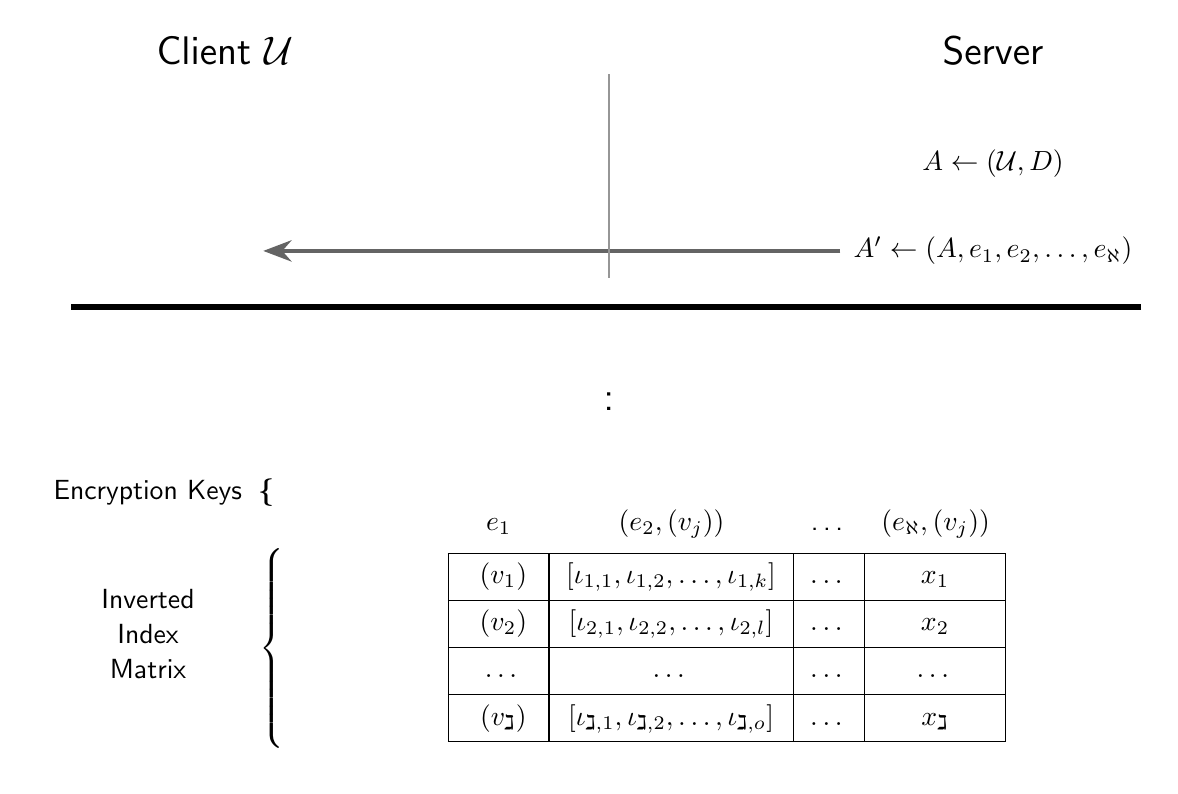
\begin{tikzpicture}[auto,>=Triangle,font=\sffamily]
        \node (server) {\Large Server};
        \node[base left=8cm of server] (client) {\Large Client $ \mathcal{U} $};
        \coordinate[below=14.79cm of server] (server_ground);
        \coordinate[below=14.79cm of client] (client_ground);
        
        \begin{scope}[line width=3pt,shift={(client_ground)},
            nodes={above}, draw=dark_gray, x={($(server_ground)-(client_ground)$)},y={($(client.south)-(client_ground)$)}]
            \draw[] (1, 0.9) node (filter) {$ A \gets \Filter \left( \mathcal{U}, D \right) $};
            \draw[] (0, 0.9) node (filter_receive) {\phantom{$ \left( A \right) $}};

            \draw[] (1, 0.825) node (garble) {$ A' \gets \Garble \left( A, e_1, e_2, \dots, e_\aleph \right) $};
            \draw[] (0, 0.825) node (garble_receive) {\phantom{$ \left( A' \right) $}};
            \draw[ultra thick, -{Stealth[scale=1]}] (garble) -- (garble_receive);

            \draw[line width=1pt, light_gray] (0.5, 1) -- (0.5, 0.825);

            \draw[-, line width=2pt, shorten <=2pt, black] (1.2, 0.8) -- (-0.2, 0.8);

            \draw[] (0.5, 0.7) node (title_garble) {\Large{$ \Garble $:}};

            \node [shape=rectangle, align=center](table1) at (0.66, 0.415) {
                \begin{tabular}{|c | c | c | c|}

                    \multicolumn{1}{c}{ \hspace*{1ex} $ e_1 $ \hspace*{1ex}} & \multicolumn{1}{c}{$ \Encrypt\left( e_2, \Hash \left( v_j \right) \right) $} & \multicolumn{1}{c}{\dots} & \multicolumn{1}{c}{ $ \Encrypt\left( e_{\aleph}, \Hash \left( v_j \right) \right) $} \\ [1ex] 
                    
                    \hline \rule{0pt}{0.9\normalbaselineskip}
                    $ \Hash\left(v_1\right) $ & $ \left[ \iota_{1, 1}, \iota_{1, 2}, \dots , \iota_{1, k}  \right] $ & $ \dots $ & $ x_1 $\\ [0.5ex]
                    \hline \rule{0pt}{0.9\normalbaselineskip}
                    $ \Hash\left(v_2\right) $ & $ \left[ \iota_{2, 1}, \iota_{2, 2}, \dots , \iota_{2, l}  \right] $ & $ \dots $ & $ x_2 $ \\ [0.5ex]
                    \hline \rule{0pt}{0.9\normalbaselineskip}
                    $ \dots $ & $ \dots $ & $ \dots $ & $ \dots $ \\ [0.5ex]
                    \hline \rule{0pt}{0.9\normalbaselineskip}
                    $ \Hash\left( v_\gimel \right) $ & $ \left[ \iota_{\gimel, 1}, \iota_{\gimel, 2}, \dots , \iota_{\gimel, o}  \right] $ & $ \dots $ & $ x_\gimel $ \\ [0.5ex] 
                    \hline
                \end{tabular}
            };

            \draw[] (-0.09, 0.615) node (title_key) {$\begin{tabular}{l}
                Encryption Keys
                \end{tabular}\bm{\big\{}$
            };
            \draw[] (-0.1, 0.53) node (title_inverted) {Inverted};
            \draw[] (-0.1, 0.5) node (title_index) {Index};
            \draw[] (-0.1, 0.47) node (title_matrix) {Matrix};
            \draw[] (0.037, 0.41) node (title_key) {$\left.\begin{tabular}{l}
                \\
                \\
                \\
                \\
                \\
                \\
                \end{tabular}\right\{$
            };

        \end{scope}
    \end{tikzpicture}
    \label{ill:KeywordSearchInitiation}
\end{figure}
\cleardoublepage
\noindent
\begin{figure} [H]
    \centering
    \captionsetup{justification=centering,margin=1cm}
    \caption*{\hspace*{1.8cm}\textbf{\LARGE{Communication Flow}}}
    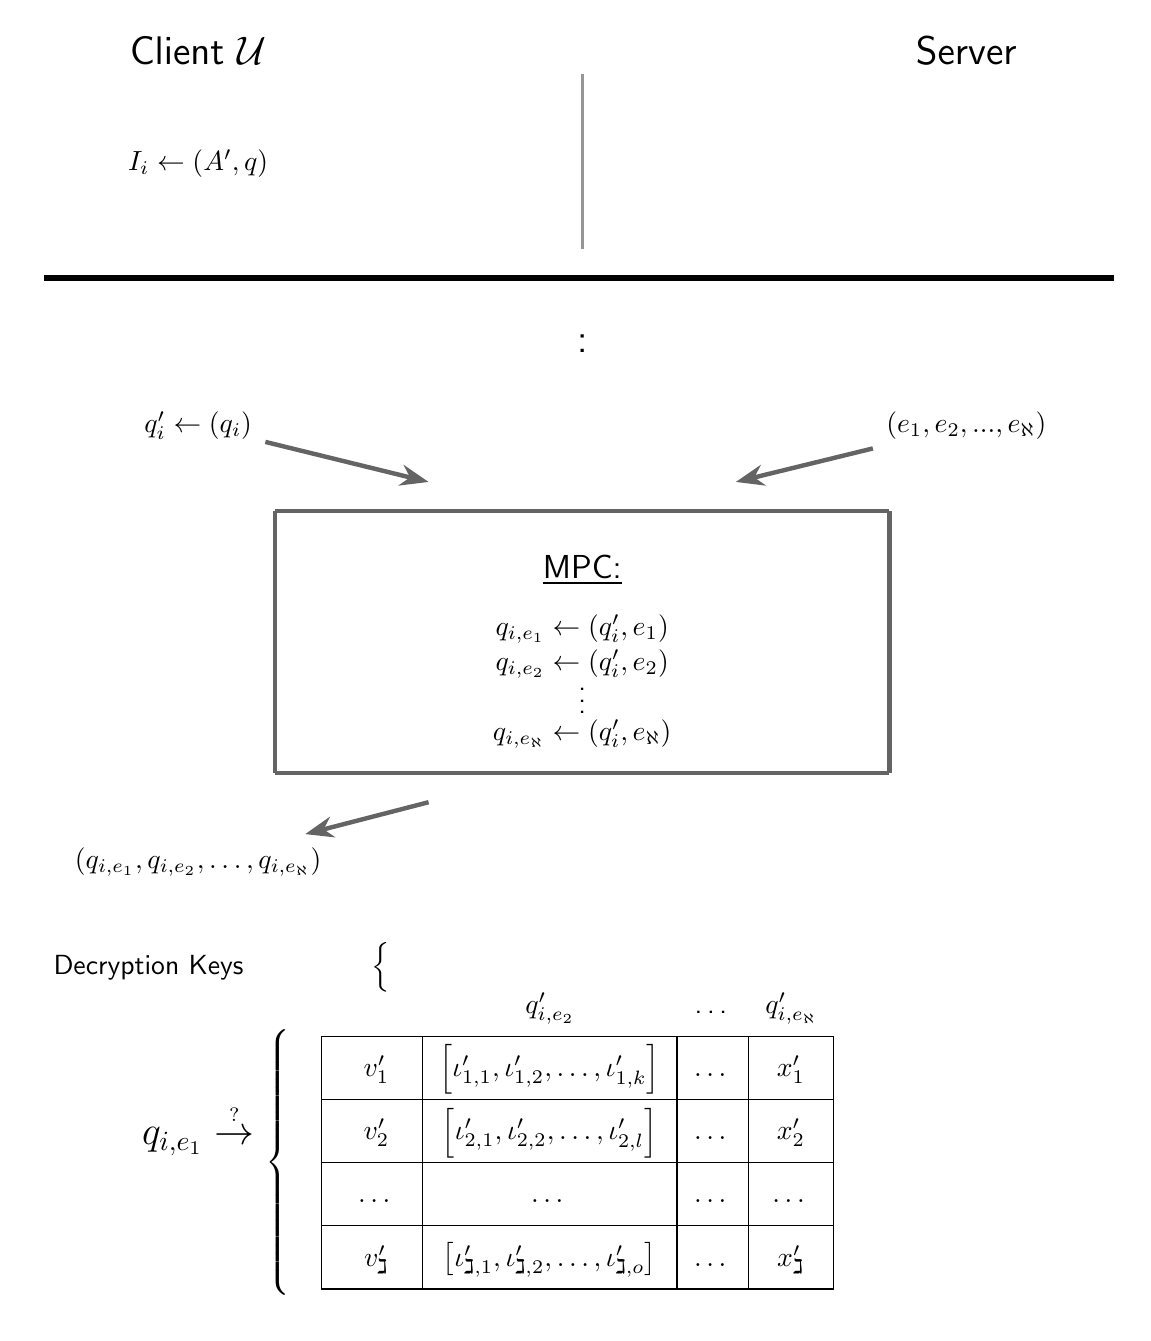
\begin{tikzpicture}[auto,>=Triangle,font=\sffamily]
        \node (server) {\Large Server};
        \node[base left=8cm of server] (client) {\Large Client $ \mathcal{U} $};
        \coordinate[below=14.79cm of server] (server_ground);
        \coordinate[below=14.79cm of client] (client_ground);
        
        \begin{scope}[line width=3pt,shift={(client_ground)},
            nodes={above}, draw=dark_gray, x={($(server_ground)-(client_ground)$)},y={($(client.south)-(client_ground)$)}]
            
            \draw[] (0, 0.9) node (filter) {$ I_i \gets \Search \left( A', q \right) $};

            \draw[line width=1pt, light_gray] (0.5, 1) -- (0.5, 0.85);

            \draw[-, line width=2pt, shorten <=2pt, black] (1.2, 0.825) -- (-0.2, 0.825);

            \draw[] (0.5, 0.75) node (title_garble) {\Large{$ \Search $:}};
            
            \draw[] (1, 0.675) node (filter) {$ \left( e_1, e_ 2, ... , e_\aleph \right) $};
            \draw[ultra thick, -{Stealth[scale=1]}] (filter) -- (0.7, 0.65);
            \draw[] (0, 0.675) node (q) { $ q'_i \gets \Hash \left( q_i \right) $};
            \draw[ultra thick, -{Stealth[scale=1]}] (q) -- (0.3, 0.65);

            \draw[ultra thick, -] (0.1, 0.625) -- (0.9, 0.625);
            \draw[ultra thick, -] (0.1, 0.625) -- (0.1, 0.4);
            \draw[ultra thick, -] (0.9, 0.625) -- (0.9, 0.4);
            \draw[ultra thick, -] (0.1, 0.4) -- (0.9, 0.4);

            \draw[] (0.5, 0.55) node {\large \underline{MPC:}};

            \draw[] (0.5, 0.5) node (encrypt1) {$ q_{i, e_1} \gets \Encrypt \left( q'_i, e_1 \right) $};
            \draw[] (0.5, 0.47) node (encrypt2) {$ q_{i, e_2} \gets \Encrypt \left( q'_i, e_2 \right) $};
            \draw[] (0.5, 0.44) node (encrypt2) {$ \vdots $};
            \draw[] (0.5, 0.41) node (encrypt2) {$ q_{i, e_\aleph} \gets \Encrypt \left( q'_i, e_\aleph \right) $};

            \draw[] (0, 0.3) node (q) {$ \left( q_{i, e_1}, q_{i, e_2}, \dots, q_{i, e_\aleph} \right) $};
            \draw[ultra thick, -{Stealth[scale=1]}] (0.3, 0.375) -- (q);

            \node [shape=rectangle, align=center](table1) at (0.5, -0.055) {
                \begin{tabular}{|c | c | c | c|}

                    \multicolumn{1}{c}{ \hspace*{1ex} \phantom{$ e_1 $} \hspace*{1ex}} & \multicolumn{1}{c}{$ q'_{i,e_2} $} & \multicolumn{1}{c}{\dots} & \multicolumn{1}{c}{ $ q'_{i,e_\aleph} $} \\ [1ex] 
                    
                    \hline \rule{0pt}{1.2\normalbaselineskip}
                    $ v'_1 $ & $ \left[ \iota'_{1, 1}, \iota'_{1, 2}, \dots , \iota'_{1, k}  \right] $ & $ \dots $ & $ x'_1 $\\ [1ex]
                    \hline \rule{0pt}{1.2\normalbaselineskip}
                    $ v'_2 $ & $ \left[ \iota'_{2, 1}, \iota'_{2, 2}, \dots , \iota'_{2, l}  \right] $ & $ \dots $ & $ x'_2 $ \\ [1ex]
                    \hline \rule{0pt}{1.2\normalbaselineskip}
                    $ \dots $ & $ \dots $ & $ \dots $ & $ \dots $ \\ [1ex]
                    \hline \rule{0pt}{1.2\normalbaselineskip}
                    $ v'_{\gimel} $ & $ \left[ \iota'_{\gimel, 1}, \iota'_{\gimel, 2}, \dots , \iota'_{\gimel, o}  \right] $ & $ \dots $ & $ x'_\gimel $ \\ [1ex] 
                    \hline
                \end{tabular}
            };

            \draw[] (0.02, 0.2) node (title_key) {$\begin{tabular}{l}
                Decryption Keys \hspace*{1.3cm}
                \end{tabular}\bm{\Big\{}$
            };
            \draw[] (0, 0.06) node (find_q) {\Large{$ q_{i,e_1} \overset{{\scriptscriptstyle?}}{\rightarrow} $}};

            \draw[] (0.08, -0.06) node (title_key) {$\left.\begin{tabular}{l}
                \\
                \\
                \\
                \\
                \\
                \\
                \\
                \\
                \end{tabular}\right\{$
            };

        \end{scope}
    \end{tikzpicture}
    \label{ill:KeywordSearchTransfer}
\end{figure}
\cleardoublepage
\noindent
\begin{figure} [H]
    \centering
    \captionsetup{justification=centering,margin=1cm}
    \caption*{\hspace*{3.3cm}\textbf{\LARGE{Communication Flow}}}
    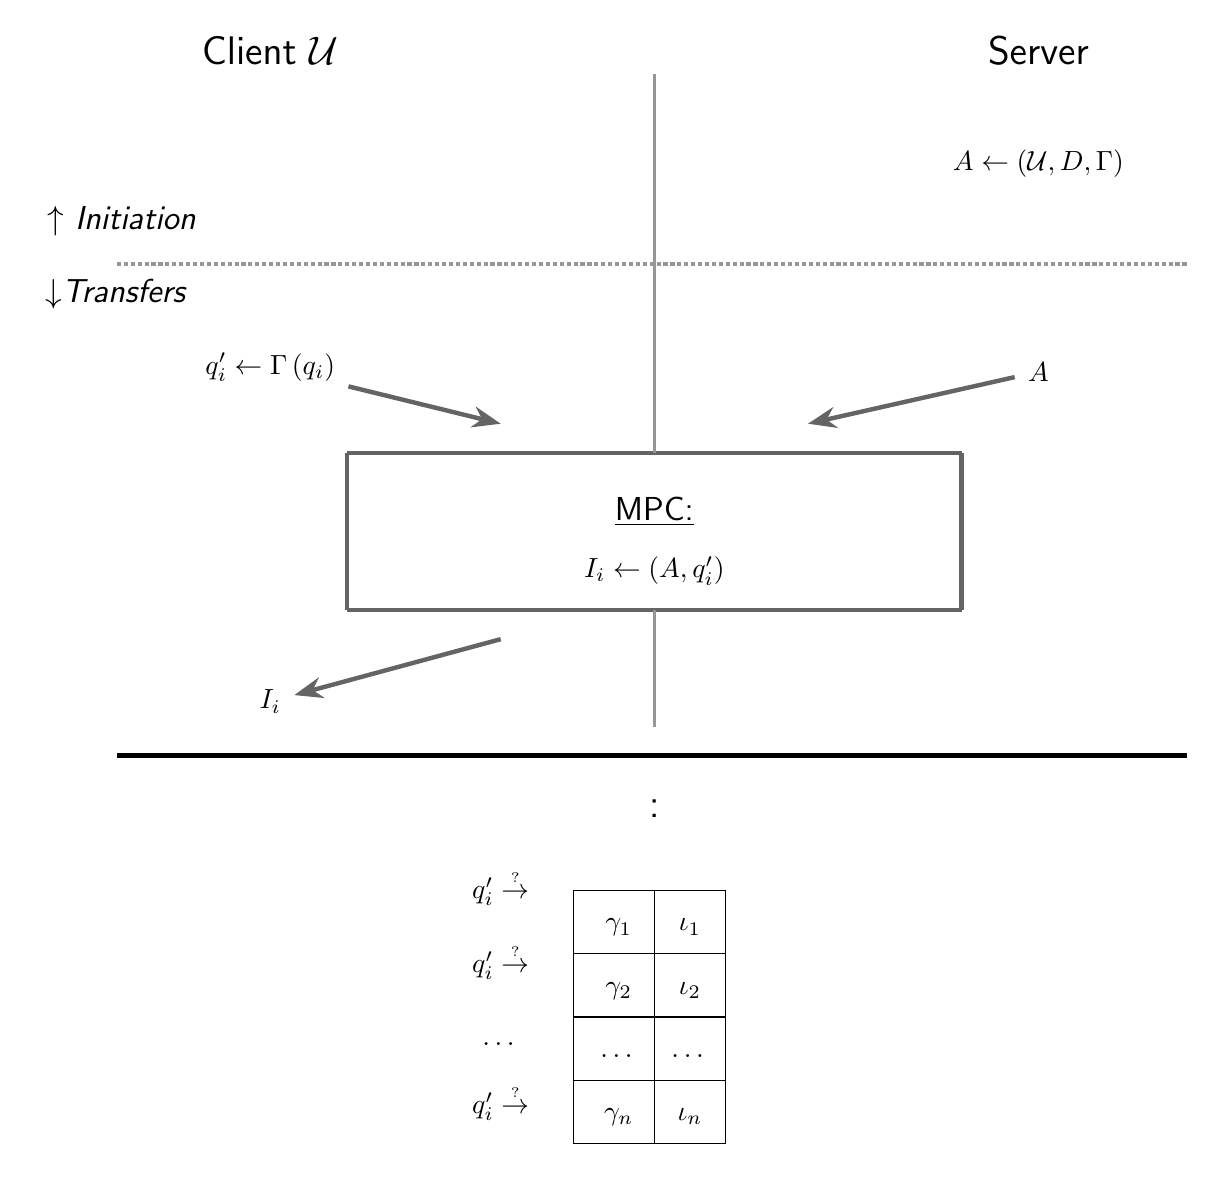
\begin{tikzpicture}[auto,>=Triangle,font=\sffamily]
        \node (server) {\Large Server};
        \node[base left=8cm of server] (client) {\Large Client $ \mathcal{U} $};
        \coordinate[below=14.79cm of server] (server_ground);
        \coordinate[below=14.79cm of client] (client_ground);
        
        \begin{scope}[line width=3pt,shift={(client_ground)},
            nodes={above}, draw=dark_gray, x={($(server_ground)-(client_ground)$)},y={($(client.south)-(client_ground)$)}]
            
            \draw[] (1, 0.9) node (filter) {$ A \gets \Filter \left( \mathcal{U}, D, \Gamma \right) $};
            \draw[] (0, 0.9) node (filter_receive) {\phantom{$ \left( A \right) $}};

            \draw[] (-0.2, 0.85) node (title_initiation) {\large{ $ \uparrow $ \textit{Initiation}}};

            \draw[densely dotted,line width=1.5pt, shorten <=2pt, light_gray] (1.2, 0.837) -- (-0.2, 0.837);

            \draw[] (-0.2, 0.787) node (title_transfers) {\large{$ \downarrow $\textit{Transfers}}};

            \draw[] (1, 0.725) node (a) {$ A $};
            \draw[ultra thick, -{Stealth[scale=1]}] (a) -- (0.7, 0.7);
            \draw[] (0, 0.725) node (q) { $ q'_i \gets \Gamma \left( q_i \right) $};
            \draw[ultra thick, -{Stealth[scale=1]}] (q) -- (0.3, 0.7);

            \draw[ultra thick, -] (0.1, 0.675) -- (0.9, 0.675);
            \draw[ultra thick, -] (0.1, 0.675) -- (0.1, 0.54);
            \draw[ultra thick, -] (0.9, 0.675) -- (0.9, 0.54);
            \draw[ultra thick, -] (0.1, 0.54) -- (0.9, 0.54);

            \draw[] (0.5, 0.6) node {\large \underline{MPC:}};

            \draw[] (0.5, 0.55) node (encrypt1) {$ I_i \gets \Search \left( A, q'_i \right) $};

            \draw[] (0, 0.44) node (I) {$ I_i $};
            \draw[ultra thick, -{Stealth[scale=1]}] (0.3, 0.515) -- (I);

            \draw[line width=1pt, light_gray] (0.5, 1) -- (0.5, 0.675);
            \draw[line width=1pt, light_gray] (0.5, 0.54) -- (0.5, 0.44);

            \draw[-, line width=2pt, shorten <=2pt, black] (1.2, 0.415) -- (-0.2, 0.415);

            \draw[] (0.5, 0.35) node (title_garble) {\Large{$ \Search $:}};

            \node [shape=rectangle, align=center](table1) at (0.5, 0.07) {
                \begin{tabular}{|c | c|}
                    
                    \hline \rule{0pt}{1.2\normalbaselineskip}
                    $ \gamma_1 $ & $ \iota_1 $ \\ [1ex]
                    \hline \rule{0pt}{1.2\normalbaselineskip}
                    $ \gamma_2 $ & $ \iota_2 $ \\ [1ex]
                    \hline \rule{0pt}{1.2\normalbaselineskip}
                    $ \dots $ & $ \dots $ \\ [1ex]
                    \hline \rule{0pt}{1.2\normalbaselineskip}
                    $ \gamma_n $ & $ \iota_n $ \\ [1ex] 
                    \hline
                \end{tabular}
            };

            \draw[] (0.3, 0.275) node (find_q) {$ q'_i \overset{{\scriptscriptstyle?}}{\rightarrow} $};

            \draw[] (0.3, 0.211) node (find_q) {$ q'_i \overset{{\scriptscriptstyle?}}{\rightarrow} $};

            \draw[] (0.3, 0.155) node (find_q) {$ \dots $};

            \draw[] (0.3, 0.09) node (find_q) {$ q'_i \overset{{\scriptscriptstyle?}}{\rightarrow} $};

        \end{scope}
    \end{tikzpicture}
    \label{ill:SemanticSearchInitiation}
\end{figure}
\cleardoublepage
\noindent
\begin{figure} [H]
    \centering
    \captionsetup{justification=centering,margin=1cm}
    \caption*{\hspace*{3.1cm}\textbf{\LARGE{Communication Flow}}}
    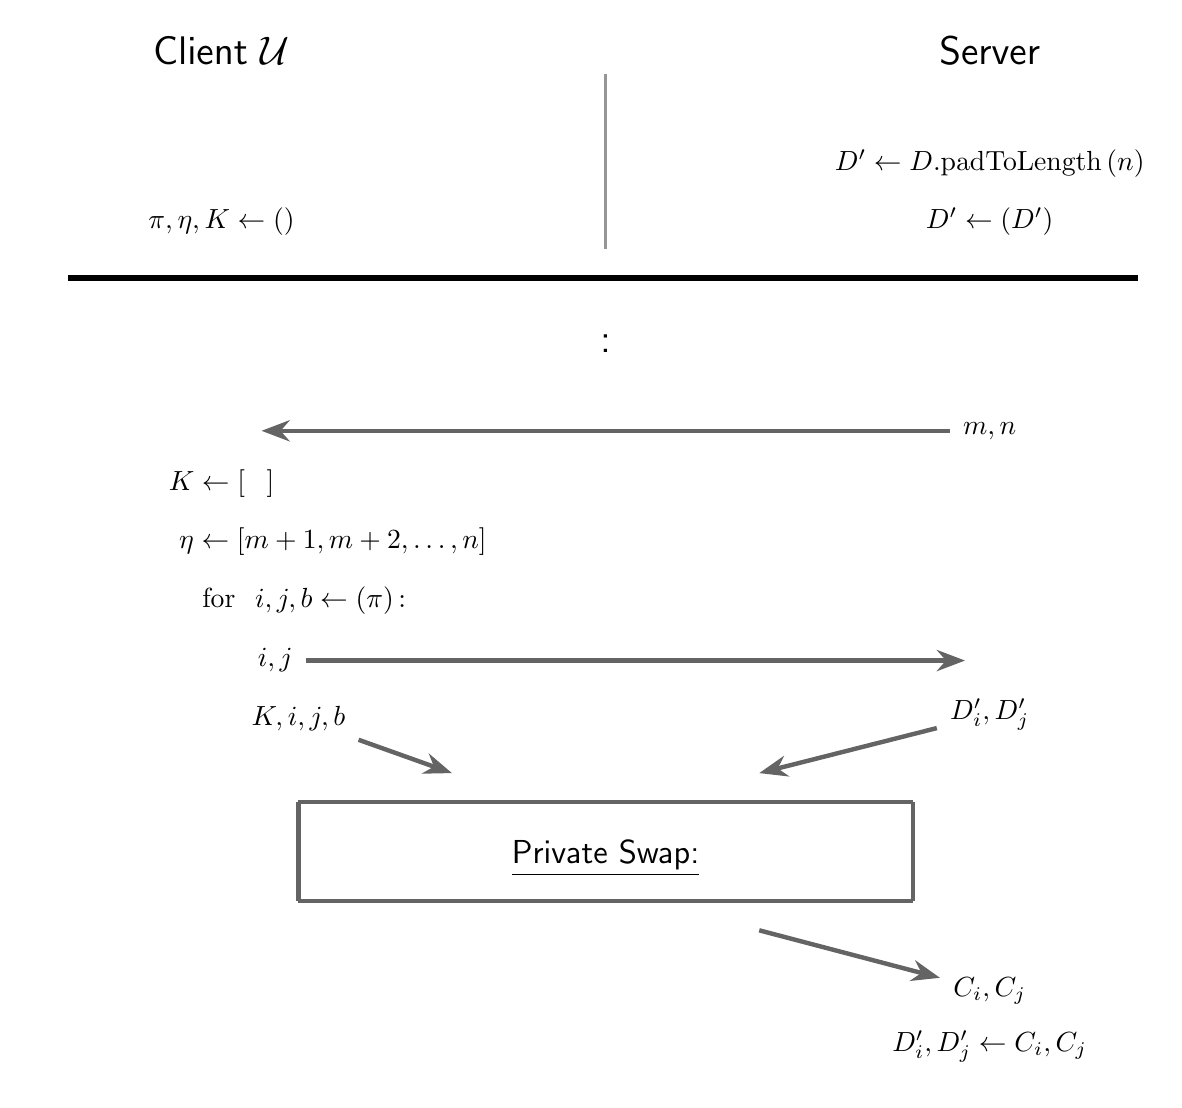
\begin{tikzpicture}[auto,>=Triangle,font=\sffamily]
        \node (server) {\Large Server};
        \node[base left=8cm of server] (client) {\Large Client $ \mathcal{U} $};
        \coordinate[below=14.79cm of server] (server_ground);
        \coordinate[below=14.79cm of client] (client_ground);
        
        \begin{scope}[line width=3pt,shift={(client_ground)},
            nodes={above}, draw=dark_gray, x={($(server_ground)-(client_ground)$)},y={($(client.south)-(client_ground)$)}]

            \draw[] (1, 0.9) node (preprocess) {$ D' \gets D.\mathrm{padToLength}\left(n\right)$};

            \draw[] (0, 0.85) node (preprocess) {$ \pi, \eta, K \gets \PreProcess \left( \right) $};
            \draw[] (1, 0.85) node (preprocess_receive) {$ D' \gets \PreProcess \left( D' \right) $};

            \draw[line width=1pt, light_gray] (0.5, 1) -- (0.5, 0.85);

            \draw[-, line width=2pt, shorten <=2pt, black] (1.2, 0.825) -- (-0.2, 0.825);

            \draw[] (0.5, 0.75) node (title_preprocess) {\Large{$ \PreProcess $:}};

            \draw[] (1, 0.675) node (mn) {$ m, n $};
            \draw[] (0, 0.675) node (mn_receive) {$ \phantom{m, n} $};
            \draw[ultra thick, -{Stealth[scale=1]}] (mn) -- (mn_receive);

            \draw[] (0, 0.625) node (preprocess) {$ K \gets \left[ \phantom{=} \right] $};

            \draw[] (0.145, 0.575) node (eta) {$ \eta \gets \left[m + 1, m + 2, \dots, n \right] $};

            \draw[] (0, 0.525) node (preprocess) {\hspace*{2.1cm}$ \mathrm{for} \hspace*{0.25cm} i,j ,b \gets \Sort\left( \pi \right)\colon $};

            \draw[] (0.07, 0.475) node (ij) {$ i, j $};
            \draw[] (1, 0.475) node (ij_receive) {$ \phantom{ij} $};
            \draw[ultra thick, -{Stealth[scale=1]}] (ij) -- (ij_receive);

            \draw[] (1, 0.425) node (a) {$ D'_i, D'_j $};
            \draw[ultra thick, -{Stealth[scale=1]}] (a) -- (0.7, 0.4);
            \draw[] (0.1, 0.425) node (q) { $ K, i, j, b $};
            \draw[ultra thick, -{Stealth[scale=1]}] (q) -- (0.3, 0.4);

            \draw[ultra thick, -] (0.1, 0.375) -- (0.9, 0.375);
            \draw[ultra thick, -] (0.1, 0.375) -- (0.1, 0.29);
            \draw[ultra thick, -] (0.9, 0.375) -- (0.9, 0.29);
            \draw[ultra thick, -] (0.1, 0.29) -- (0.9, 0.29);

            \draw[] (0.5, 0.3) node {\large \underline{Private Swap:}};

            \draw[] (1, 0.19) node (I) {$ C_i, C_j $};
            \draw[ultra thick, -{Stealth[scale=1]}] (0.7, 0.265) -- (I);

            \draw[] (1, 0.14) node (I) {$ D'_i, D'_j \gets C_i, C_j $};



        \end{scope}
    \end{tikzpicture}
    \label{ill:FileRetrievalInitiation}
\end{figure}
\cleardoublepage
\noindent
\begin{figure} [H]
    \centering
    \captionsetup{justification=centering,margin=1cm}
    \caption*{\hspace*{1.4cm}\textbf{\LARGE{Communication Flow}}}
    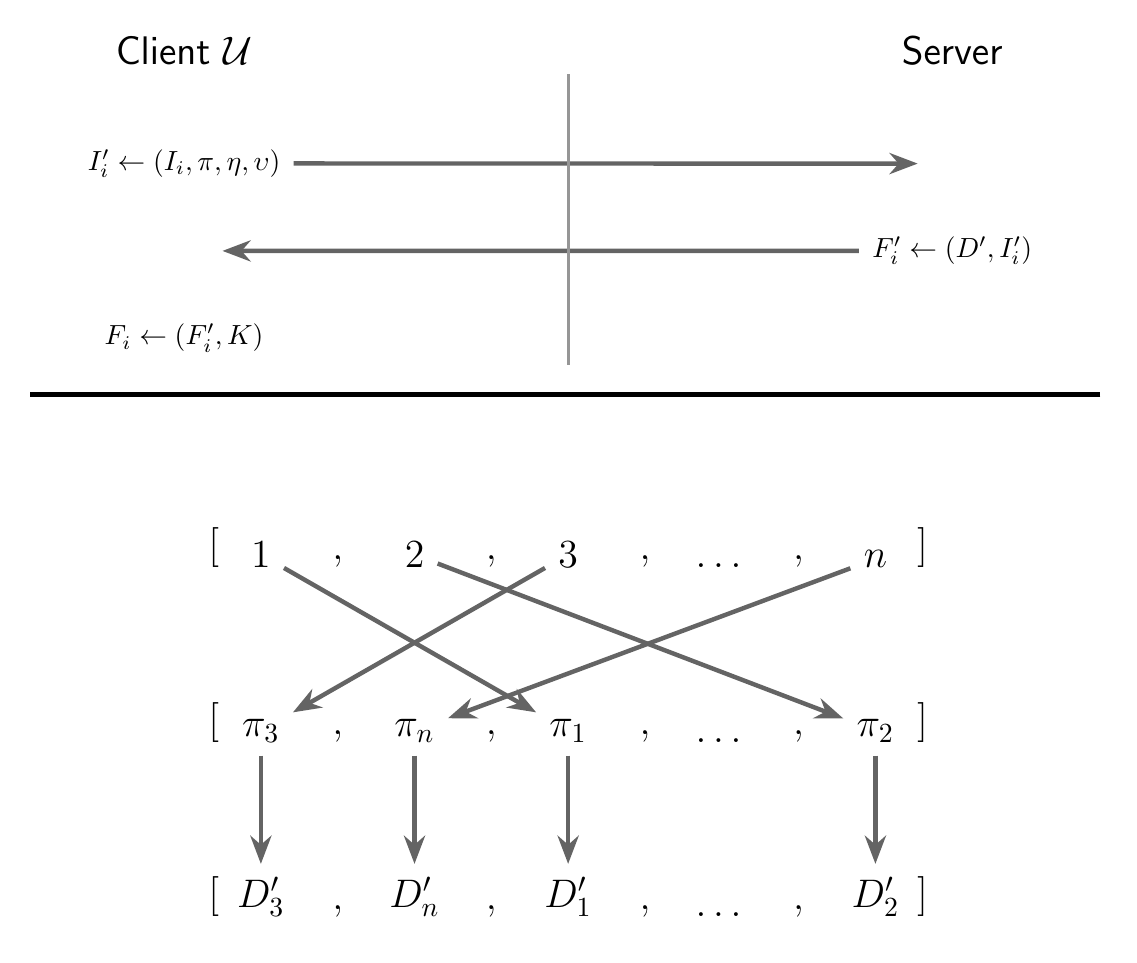
\begin{tikzpicture}[auto,>=Triangle,font=\sffamily]
        \node (server) {\Large Server};
        \node[base left=8cm of server] (client) {\Large Client $ \mathcal{U} $};
        \coordinate[below=14.79cm of server] (server_ground);
        \coordinate[below=14.79cm of client] (client_ground);
        
        \begin{scope}[line width=3pt,shift={(client_ground)},
            nodes={above}, draw=dark_gray, x={($(server_ground)-(client_ground)$)},y={($(client.south)-(client_ground)$)}]
            \draw[] (0, 0.9) node (encode) {$ I'_i \gets \Encode \left( I_i, \pi, \eta, \upsilon \right) $};
            \draw[] (1, 0.9) node (encode_receive) {\phantom{$ \left( A \right) $}};
            \draw[ultra thick, -{Stealth[scale=1]}] (encode) -- (encode_receive);

            \draw[] (1, 0.825) node (garble) {$ F'_i \gets \Retrieve \left( D', I'_i \right) $};
            \draw[] (0, 0.825) node (garble_receive) {\phantom{$ \left( A' \right) $}};
            \draw[ultra thick, -{Stealth[scale=1]}] (garble) -- (garble_receive);

            \draw[] (0, 0.75) node (decode) {$ F_i \gets \Decode \left( F'_i, K \right) $};
            \draw[] (1, 0.75) node (decode_receive) {\phantom{$ \left( A' \right) $}};


            \draw[line width=1pt, light_gray] (0.5, 1) -- (0.5, 0.75);

            \draw[-, line width=2pt, shorten <=2pt, black] (1.2, 0.725) -- (-0.2, 0.725);

            \draw[] (0.075, 0.565) node (indices) {\Large{$ [ \phantom{R_1,} $}};
            \draw[] (0.1, 0.565) node (index_1) {\Large{$ 1 $}};
            \draw[] (0.2, 0.565) node (index) {\Large{$ , $}};
            \draw[] (0.3, 0.565) node (index_2) {\Large{$ 2 $}};
            \draw[] (0.4, 0.565) node (index) {\Large{$ , $}};
            \draw[] (0.5, 0.565) node (index_3) {\Large{$ 3 $}};
            \draw[] (0.6, 0.565) node (index) {\Large{$ , $}};
            \draw[] (0.7, 0.565) node (index) {\Large{$ \dots $}};
            \draw[] (0.8, 0.565) node (index) {\Large{$ , $}};
            \draw[] (0.9, 0.565) node (index_n) {\Large{$ n $}};
            \draw[] (0.925, 0.565) node (indices) {\Large{$ \phantom{R_1,} ] $}};

            \draw[] (0.075, 0.415) node (indices) {\Large{$ [ \phantom{R_1,} $}};
            \draw[] (0.1, 0.415) node (perm_3) {\Large{$ \pi_3 $}};
            \draw[] (0.2, 0.415) node (perm) {\Large{$ , $}};
            \draw[] (0.3, 0.415) node (perm_n) {\Large{$ \pi_n $}};
            \draw[] (0.4, 0.415) node (perm) {\Large{$ , $}};
            \draw[] (0.5, 0.415) node (perm_1) {\Large{$ \pi_1 $}};
            \draw[] (0.6, 0.415) node (perm) {\Large{$ , $}};
            \draw[] (0.7, 0.415) node (perm) {\Large{$ \dots $}};
            \draw[] (0.8, 0.415) node (perm) {\Large{$ , $}};
            \draw[] (0.9, 0.415) node (perm_2) {\Large{$ \pi_2 $}};
            \draw[] (0.925, 0.415) node (indices) {\Large{$ \phantom{R_1,} ] $}};
            \draw[ultra thick, -{Stealth[scale=1]}] (index_1) -- (perm_1);
            \draw[ultra thick, -{Stealth[scale=1]}] (index_2) -- (perm_2);
            \draw[ultra thick, -{Stealth[scale=1]}] (index_3) -- (perm_3);
            \draw[ultra thick, -{Stealth[scale=1]}] (index_n) -- (perm_n);

            \draw[] (0.075, 0.265) node (indices) {\Large{$ [ \phantom{R_1,} $}};
            \draw[] (0.1, 0.265) node (record_3) {\Large{$ D'_3 $}};
            \draw[] (0.2, 0.265) node (record) {\Large{$ , $}};
            \draw[] (0.3, 0.265) node (record_n) {\Large{$ D'_n $}};
            \draw[] (0.4, 0.265) node (record) {\Large{$ , $}};
            \draw[] (0.5, 0.265) node (record_1) {\Large{$ D'_1 $}};
            \draw[] (0.6, 0.265) node (record) {\Large{$ , $}};
            \draw[] (0.7, 0.265) node (record) {\Large{$ \dots $}};
            \draw[] (0.8, 0.265) node (record) {\Large{$ , $}};
            \draw[] (0.9, 0.265) node (record_2) {\Large{$ D'_2 $}};
            \draw[] (0.925, 0.265) node (indices) {\Large{$ \phantom{R_1,} ] $}};
            \draw[ultra thick, -{Stealth[scale=1]}] (perm_1) -- (record_1);
            \draw[ultra thick, -{Stealth[scale=1]}] (perm_2) -- (record_2);
            \draw[ultra thick, -{Stealth[scale=1]}] (perm_3) -- (record_3);
            \draw[ultra thick, -{Stealth[scale=1]}] (perm_n) -- (record_n);

        \end{scope}
    \end{tikzpicture}
    \label{ill:FileRetrievalTransfer}
\end{figure}

\end{document}
